 \documentclass[11pt,twoside,a4paper]{article}

\usepackage[polish]{babel}
\usepackage{polski}
\usepackage[utf8]{inputenc}
\usepackage[OT4]{fontenc}
\usepackage{tgtermes}	%Times New Roman
\usepackage[left=2.5cm,top=2.5cm,right=2.5cm,bottom=2.5cm,
headsep=0.5cm,headheight=1.0cm,marginpar=2cm,reversemp]{geometry}
\usepackage{fancyhdr}
\usepackage[table]{xcolor}
\usepackage{graphicx}
\usepackage{amsmath}
\usepackage{amsthm,thmtools}
\usepackage[nottoc]{tocbibind}
\usepackage{ragged2e}
\usepackage{bbding}
\usepackage{makeidx}
\usepackage{titlesec}
\usepackage{tcolorbox}
\usepackage{url}
\usepackage{color}
\usepackage{setspace}
\usepackage[font=small,format=plain,labelfont=bf,up,textfont=it,up]{caption}
\usepackage{BeamerColor}
\usepackage{listings}
\usepackage{pdfpages}
\usepackage{hyperref}

\definecolor{mycolor1}{RGB}{0,0,128}
\definecolor{lightgray}{gray}{0.9}
\definecolor{lightlightgray}{gray}{0.95}
\definecolor{lightyellow}{RGB}{255,255,224}
\definecolor{lemonchiffon}{RGB}{255,250,205}



\newcommand{\mat}[1]{\boldsymbol{\mathrm{#1}}}

\hypersetup{
	pdftitle={Metody Programowania Robotów},
	pdfauthor={Pawe\l{} Malczyk, Pawe\l{} Tomulik},
	pdfkeywords={systemy operacyjne czasu rzeczywistego, QNX, robot},
	pdfsubject={Zestaw instrukcji laboratoryjnych QNX}
	pageanchor=true,
	breaklinks=true,
	plainpages=false,
	linktocpage=true
}
% zmiana nazw domyślnych
\addto\captionspolish
{
	\renewcommand{\tablename}{Tabela}
	\renewcommand{\listtablename}{Spis tabel}
	\renewcommand{\bibname}{Piśmiennictwo}
	\renewcommand{\chaptername}{Laboratorium}
}


%\newtheoremstyle{mystyle}% name of the style to be used
%  {12pt}% measure of space to leave above the theorem. E.g.: 3pt
%  {12pt}% measure of space to leave below the theorem. E.g.: 3pt
%  {\itshape}% name of font to use in the body of the theorem
%  {6pt}% measure of space to indent
%  {\bfseries}% name of head font
%  {\newline}% punctuation between head and body
%  {.5em}% space after theorem head; " " = normal interword space
%  {}% Manually specify head
%\theoremstyle{mystyle}
%\newtheorem{example}{\color{black}Przykład}[section]


\declaretheoremstyle[
spaceabove=6pt, spacebelow=6pt,
headfont=\normalfont\bfseries,
notefont=\mdseries,
notebraces={[}{]},
%bodyfont=\itshape,
postheadspace=1em,
%qed=\qedsymbol
]{mystyle}
\declaretheorem[name=Przykład,numberwithin=subsection,style=mystyle]{example}
%\declaretheorem[name=Definition]{definition}



%\definecolor{lightyellow}{RGB}{255,255,224}
%\definecolor{lemonchiffon}{RGB}{255,250,205}
\definecolor{syntax}{RGB}{127,0,85}
\definecolor{comments}{RGB}{63,127,95}
\definecolor{strings}{RGB}{42,0,255}

\lstdefinestyle{MyCStyle} {
    language=C, % choose the language of the code
    alsolanguage=C++,
    basicstyle=\linespread{0.9}\fontfamily{lmss}\selectfont\small\color{black},
    keywordstyle={\bfseries\color{syntax}}, % style for keywords
    emph={int,char,double,float,unsigned,printf},
    emphstyle={\bfseries\color{syntax}},
    stringstyle=\color{strings},
    commentstyle={\fontfamily{lmss}\selectfont\color{comments}},
    numbers=left, % where to put the line-numbers
    numberstyle=\tiny, % the size of the fonts that are used for the line-numbers
    backgroundcolor=\color{lemonchiffon},
%    backgroundcolor=\color{lightgray},
    showspaces=false, % show spaces adding particular underscores
    showstringspaces=false, % underline spaces within strings
    showtabs=false, % show tabs within strings adding particular underscores
    frame=single, % adds a frame around the code
    tabsize=2, % sets default tabsize to 2 spaces
    rulesepcolor=\color{gray},
    rulecolor=\color{black},
    captionpos=t, % sets the caption-position to bottom
    breaklines=true, % sets automatic line breaking
    breakatwhitespace=false,
    xleftmargin=20pt,
    xrightmargin=20pt,
    aboveskip=12pt,
    belowskip=12pt,
    escapeinside={(*@}{@*)},
%   frameround=tttt,
   framexleftmargin=5mm,
   frame=shadowbox,
   rulesepcolor=\color{lightgray},
   extendedchars=\true,
   inputencoding=utf8,
}

\lstdefinestyle{MyBashStyle} {
    language=bash, % choose the language of the code
    basicstyle=\linespread{0.9}\fontfamily{lmss}\selectfont\small\color{black},
    keywordstyle={\color{black}}, % style for keywords
    emph={},
    emphstyle={\color{black}},
    stringstyle=\color{black},
    commentstyle={\fontfamily{lmss}\selectfont\color{black}},
    numbers=left, % where to put the line-numbers
    numberstyle=\tiny, % the size of the fonts that are used for the line-numbers
    backgroundcolor=\color{lemonchiffon},
%    backgroundcolor=\color{lightgray},
    showspaces=false, % show spaces adding particular underscores
    showstringspaces=false, % underline spaces within strings
    showtabs=false, % show tabs within strings adding particular underscores
    frame=single, % adds a frame around the code
    tabsize=2, % sets default tabsize to 2 spaces
    rulesepcolor=\color{gray},
    rulecolor=\color{black},
    captionpos=t, % sets the caption-position to bottom
    breaklines=true, % sets automatic line breaking
    breakatwhitespace=false,
    xleftmargin=20pt,
    xrightmargin=20pt,
    aboveskip=12pt,
    belowskip=12pt,
    escapeinside={(*@}{@*)},
%   frameround=tttt,
   framexleftmargin=5mm,
   frame=shadowbox,
   rulesepcolor=\color{lightgray},
   extendedchars=\true,
   inputencoding=utf8,
}



\renewcommand*\lstlistingname{Kod źródłowy}
\renewcommand{\qedsymbol}{\rule{1ex}{1ex}}


%\lstset{language=Fortran, numbers=left, numberstyle=\tiny, stepnumber=1, numbersep=0pt, tabsize=5,keywordstyle=\color{black}\bfseries,aboveskip=10pt,belowskip=36pt,
%xleftmargin=20pt,xrightmargin=20pt}
%\lstset{emph={Procedura,Oblicz},emphstyle={\color{black}\bfseries},
%label=list1}
%\renewcommand*\lstlistingname{Tekst programu}
%
%\begin{lstlisting}[frame=lines,caption={Pseudokod algorytmu dziel i~zdobywaj z~dyrektywami kompilatora OpenMP}]
%\end{lstlisting}


\renewcommand{\labelitemi}{$\bullet$}
%\renewcommand{\labelitemii}{$\cdot$}
%\renewcommand{\labelitemiii}{$\diamond$}
%\renewcommand{\labelitemiv}{$\ast$}

% Wielkosc wciecia akapitowego
\parindent=0.5cm
% Odstepy miedzy akapitami
\parskip=6pt

% Uklad strony
% \pagestyle{empty}
\fancyhead{}
\pagestyle{fancy}
% Naglowki na stronie parzystej (E) i nieparzystej (O) , Right Left Center
%\fancyhead[CO]{\small \nouppercase{\textbf\rightmark}}
%\fancyhead[CE]{\small \nouppercase{\textbf\leftmark}}

%\lhead{\textbf{\small{\leftmark}}}
%\rhead{\small{Pawel Malczyk}}
%\lfoot{\textbf{\tiny{Konspekt do Podstaw Automatyki i Sterowania II}}}
%\rfoot{}

\fancyhead[CE]{\small \nouppercase{\textbf\leftmark}}
\fancyhead[CO]{\small \nouppercase{\textbf{Metody Programowania Robotów (QNX RTOS)}}}

\fancyfoot[RE,RO]{\footnotesize Paweł Malczyk, Paweł Tomulik}
\fancyfoot[LE,LO]{\footnotesize Rozpowszechnianie bez zgody autorów zabronione}
%\fancyfoot[RE,RO]{\footnotesize Rozpowszechnianie bez zgody autorów zabronione}

\linespread{1.0}
\title{\vspace{4.25cm}\Huge{\textbf{Metody Programowania Robotów}} \\ \vskip10pt\LARGE{\textit{Zestaw instrukcji laboratoryjnych do programowania aplikacji w~systemie operacyjnym czasu rzeczywistego QNX Neutrino}}}
\author{\Large{\textbf{Paweł Malczyk, Paweł Tomulik}}\vspace{0.5cm} \\ Zakład Teorii Maszyn i Robotów \\
Instytut Techniki Lotniczej i Mechaniki Stosowanej \\
Wydział Mechaniczny Energetyki i Lotnictwa \\
Politechnika Warszawska \\
{\href{mailto:pmalczyk@meil.pw.edu.pl}{pmalczyk@meil.pw.edu.pl}}, \href{mailto:ptomulik@meil.pw.edu.pl}{ptomulik@meil.pw.edu.pl} \\ www: \href{http://ztmir.meil.pw.edu.pl}{http://ztmir.meil.pw.edu.pl}}
\date{październik 2015 r.}

\linespread{1.3}

%  \titleformat{<command>}[<shape>]{<format>}{<label>}{<sep>}{<before-code>}[<after-code>]


\titleformat
{\section}
[display]
{\color{black}\normalfont\Large\bfseries\centering}
{\color{black}{\rule{\textwidth}{1pt}\\ \LARGE Laboratorium~\thesection}}
{-1em}
{
    %\rule{\textwidth}{1pt}
    \vspace{1ex}
    \centering
}
[
\vspace{-2.5ex}%
\rule{\textwidth}{0.3pt}
] % after-code

\titleformat{\subsection}
{\color{black}\normalfont\Large\bfseries}
{\color{black}\thesubsection}{1em}{}

\newenvironment{myitemize}
{ \begin{itemize}
    \setlength{\itemsep}{0pt}
    \setlength{\parskip}{0pt}
    \setlength{\parsep}{0pt}     }
{ \end{itemize}                  }

\newenvironment{myenumerate}
{ \begin{enumerate}
    \setlength{\itemsep}{0pt}
    \setlength{\parskip}{0pt}
    \setlength{\parsep}{0pt}     }
{ \end{enumerate}                  }


\begin{document}
\maketitle
\cleardoublepage

\section{Podstawy obsługi systemu operacyjnego QNX RTOS}

\subsection{Powłoka}

Powłoka:

\begin{myitemize}
\item Interpreter poleceń użytkownika
\item Pośredniczy między użytkownikiem a systemem
\item Środowisko pracy użytkownika w systemie
\item Przetwarza pojedyncze polecenia lub skrypty
\end{myitemize}


\begin{example}[Przykład prostej komendy] \label{ex:prostakomenda}

Polecenia można wydawać powłoce z wiersza poleceń (terminala, konsoli) wpisując ich nazwy.

\begin{lstlisting}[style=MyBashStyle]
# ls
\end{lstlisting}

Komenda wyświetla zawartość bieżącego katalogu.
\end{example}

\begin{example}[Przykład komendy z~argumentami]\label{ex:prostakomenda2}
%\addcontentsline{toc}{subsubsection}{Przykład \ref{ex:prostakomenda2}}

Komenda wyświetla zawartość bieżącego katalogu wraz ze szczegółowymi informacjami nt. obiektów. Argumenty (\lstinline[style=MyBashStyle]{-l}) zmieniają zachowanie komendy prostej.

\begin{lstlisting}[style=MyBashStyle]
# ls -l
\end{lstlisting}


Formalna składnia komendy z argumentami:

\begin{lstlisting}[style=MyBashStyle]
# command argument1 argument2 argument3 ... argumentN
\end{lstlisting}
\end{example}

\begin{example}[Przykład złożonej komendy]\label{ex:prostakomenda3}

Komendy proste i~komendy proste z~argumentami możemy łączyć. Separatorem poleceń jest średnik (\lstinline[style=MyBashStyle]{;}).


\begin{lstlisting}[style=MyBashStyle]
# date ; ls
\end{lstlisting}

Formalna składnia złożonej komendy:

\begin{lstlisting}[style=MyBashStyle]
# command1; command2; command3; ... argumentN
\end{lstlisting}
\end{example}

%\begin{example}[Logowanie do systemu z wiersza poleceń]\label{ex:prostakomenda4}
%
%
%Aby zalogować się do systemu z wiersza poleceń używamy polecenia \lstinline[style=MyBashStyle]{login}.
%
%\begin{lstlisting}[style=MyBashStyle]
%# login
%# login: root
%\end{lstlisting}
%
%Polecenie uzyskuje od użytkownika jego nazwę oraz hasło, które następnie weryfikuje z danymi zawartymi w pliku \lstinline[style=MyBashStyle]{/etc/passwd}, który możemy podejrzeć poleceniem \lstinline[style=MyBashStyle]{cat}.
%\end{example}
%
%
%\begin{example}[Plik definiujący użytkowników systemu]\label{ex:prostakomenda5}
%
%
%Po zalogowaniu przez polecenie \lstinline[style=MyBashStyle]{login} wywoływana jest powłoka (\lstinline[style=MyBashStyle]{/bin/sh}). Następnie w fazie inicjalizacji, ustawiane są parametry pracy powłoki. Na ogół jest to proces dwuetapowy, w~którym interpretowane są pliki \lstinline[style=MyBashStyle]{/etc/passwd} oraz \lstinline[style=MyBashStyle]{.profile} z domowego katalogu. Obejrzeć zawrtość pliku \lstinline[style=MyBashStyle]{/etc/passwd}.
%
%\begin{lstlisting}[style=MyBashStyle]
%# cat /etc/passwd
%\end{lstlisting}
%\end{example}

\begin{example}[Wejście i wyjście z powłoki]\label{ex:prostakomenda6}


Powłoka wykonuje polecenia użytkownika. Kiedy powłoka wyświetla znak zachęty, który w domyślnym shell-u (Bourne shell) w systemie QNX jest znak \lstinline[style=MyBashStyle]{#} dla użytkownika \lstinline[style=MyBashStyle]{root}, to czeka na polecenia użytkownika. Możemy uruchomić powłokę w takim trybie. Sytuację tę ilustruje poniższy przykład.


\begin{lstlisting}[style=MyBashStyle]
# /bin/sh
#
# exit
\end{lstlisting}

Aby wyjść z powłoki należy użyć polecenia \lstinline[style=MyBashStyle]{# exit}.
\end{example}

\begin{example}[Obsługa edytora tekstu vi]\label{ex:vi}


Edytor \lstinline[style=MyBashStyle]{vi} jest zaawansowanym edytorem tekstowym często występującym w~systemach Unix. Aby uruchomić edytor należy wpisać komendę:

\begin{lstlisting}[style=MyBashStyle]
# vi
\end{lstlisting}

 Edytor \lstinline[style=MyBashStyle]{vi} jest edytorem modalnym. Oznacza to, że może znajdować się w~dwóch stanach: \textbf{trybie edycji} lub \textbf{trybie poleceń}.

\begin{myitemize}
\item Przejście do trybu edycji poprzez wydanie polecenia \lstinline[style=MyBashStyle]{i} (insert) lub \lstinline[style=MyBashStyle]{a} (append).
\item Przejcie z~trybu edycji do trybu poleceń odbywa się poprzez naciśnięcie klawicza \lstinline[style=MyBashStyle]{Esc}.
\end{myitemize}

Polecenia edytora \lstinline[style=MyBashStyle]{vi} składają się z~kilku grup. Przedstawiono je zbiorczo w~postaci krótkiej instrukcji na stronie~\pageref{viRef}.

W~trybie edycji, tj. po wciśnięciu klawisza \lstinline[style=MyBashStyle]{i} wpiszmy do pliku następujące linie tekstu postaci, np.:


\begin{lstlisting}[style=MyBashStyle]
Jak dobrze wstac
Skoro swit
Jutrzenki blask
Duszkiem pic
Tytul:
Radosc o poranku
Nim w gorze tam
Skowronek zacznie tryl
Jak dobrze wczesnie wstac
Dla tych chwil
\end{lstlisting}

W~następnej kolejności przejść do trybu poleceń, poprzez wciśnięcie klawisza \lstinline[style=MyBashStyle]{Esc} oraz zapisać plik wydając polecenie:

\begin{lstlisting}[style=MyBashStyle]
:w plikPoranny
\end{lstlisting}

Kolejno, zamknąć zapisany plik komendą:

\begin{lstlisting}[style=MyBashStyle]
:q
\end{lstlisting}

Otworzyć ponownie plik:

\begin{lstlisting}[style=MyBashStyle]
vi plikPoranny
\end{lstlisting}

Wykonać następujące eksperymenty:

\begin{myitemize}
\item Wykasować tekst \lstinline[style=MyBashStyle]{Tytul:} litera po literze poleceniem \lstinline[style=MyBashStyle]{x}.
\item Klawiszami \lstinline[style=MyBashStyle]{h}, \lstinline[style=MyBashStyle]{j}, \lstinline[style=MyBashStyle]{k}, \lstinline[style=MyBashStyle]{l} przejść do linii z tekstem \lstinline[style=MyBashStyle]{Radosc o poranku}.
\item Wykasować bieżącą linię za pomocą komendy \lstinline[style=MyBashStyle]{dd}. Wykasować także pustą linię, powstałą po tekście \lstinline[style=MyBashStyle]{Tytul:}.
\item Przejść do pierwszej linii pliku (\lstinline[style=MyBashStyle]{h}, \lstinline[style=MyBashStyle]{j}, \lstinline[style=MyBashStyle]{k}, \lstinline[style=MyBashStyle]{l}) i~wkleić usunięty tekst kombinacją klawiszy \lstinline[style=MyBashStyle]{Shift + P}, tak, aby cały tekst wyglądał następująco:
\end{myitemize}

\begin{lstlisting}[style=MyBashStyle]
Radosc o poranku
Jak dobrze wstac
Skoro swit
Jutrzenki blask
Duszkiem pic
Nim w gorze tam
Skowronek zacznie tryl
Jak dobrze wczesnie wstac
Dla tych chwil
\end{lstlisting}

Przeprowadzić kolejne eksperymenty:

\begin{myitemize}
\item W~trybie poleceń, znaleźć wszystkie wystąpienia słowa \lstinline[style=MyBashStyle]{dobrze} wpisując:
\end{myitemize}

\begin{lstlisting}[style=MyBashStyle]
/dobrze
\end{lstlisting}
\begin{myitemize}
\item Przeszukać tekst w~przód poprzez naciśnięcie klawisza \lstinline[style=MyBashStyle]{N}. Przeszukiwanie w~tył nastąpi poprzez wciśnięcie klawisza \lstinline[style=MyBashStyle]{Shift + N}.
\item Przejść do pierwszej linii poleceniem \lstinline[style=MyBashStyle]{:1} oraz zamienić tekst \lstinline[style=MyBashStyle]
{Radosc} na \lstinline[style=MyBashStyle]{Tytul: Radosc} poprzez sekwencję:
\end{myitemize}

\begin{lstlisting}[style=MyBashStyle]
:s/Radosc/Tytul: Radosc
\end{lstlisting}

\begin{myitemize}
\item Zamienić wszystkie wystąpienia słowa \lstinline[style=MyBashStyle]{dobrze} na \lstinline[style=MyBashStyle]{DOBRZE} w zakresie od bieżącej linii \lstinline[style=MyBashStyle]{.} do ostatniej linii \lstinline[style=MyBashStyle]{$}:
\end{myitemize}

\begin{lstlisting}[style=MyBashStyle]
:.,$s/dobrze/DOBRZE
\end{lstlisting}

Zapisać i~zamknąć plik poleceniem:

\begin{lstlisting}[style=MyBashStyle]{h}
:wq!
\end{lstlisting}
\end{example}

\clearpage
\phantomsection
{\label{viRef}
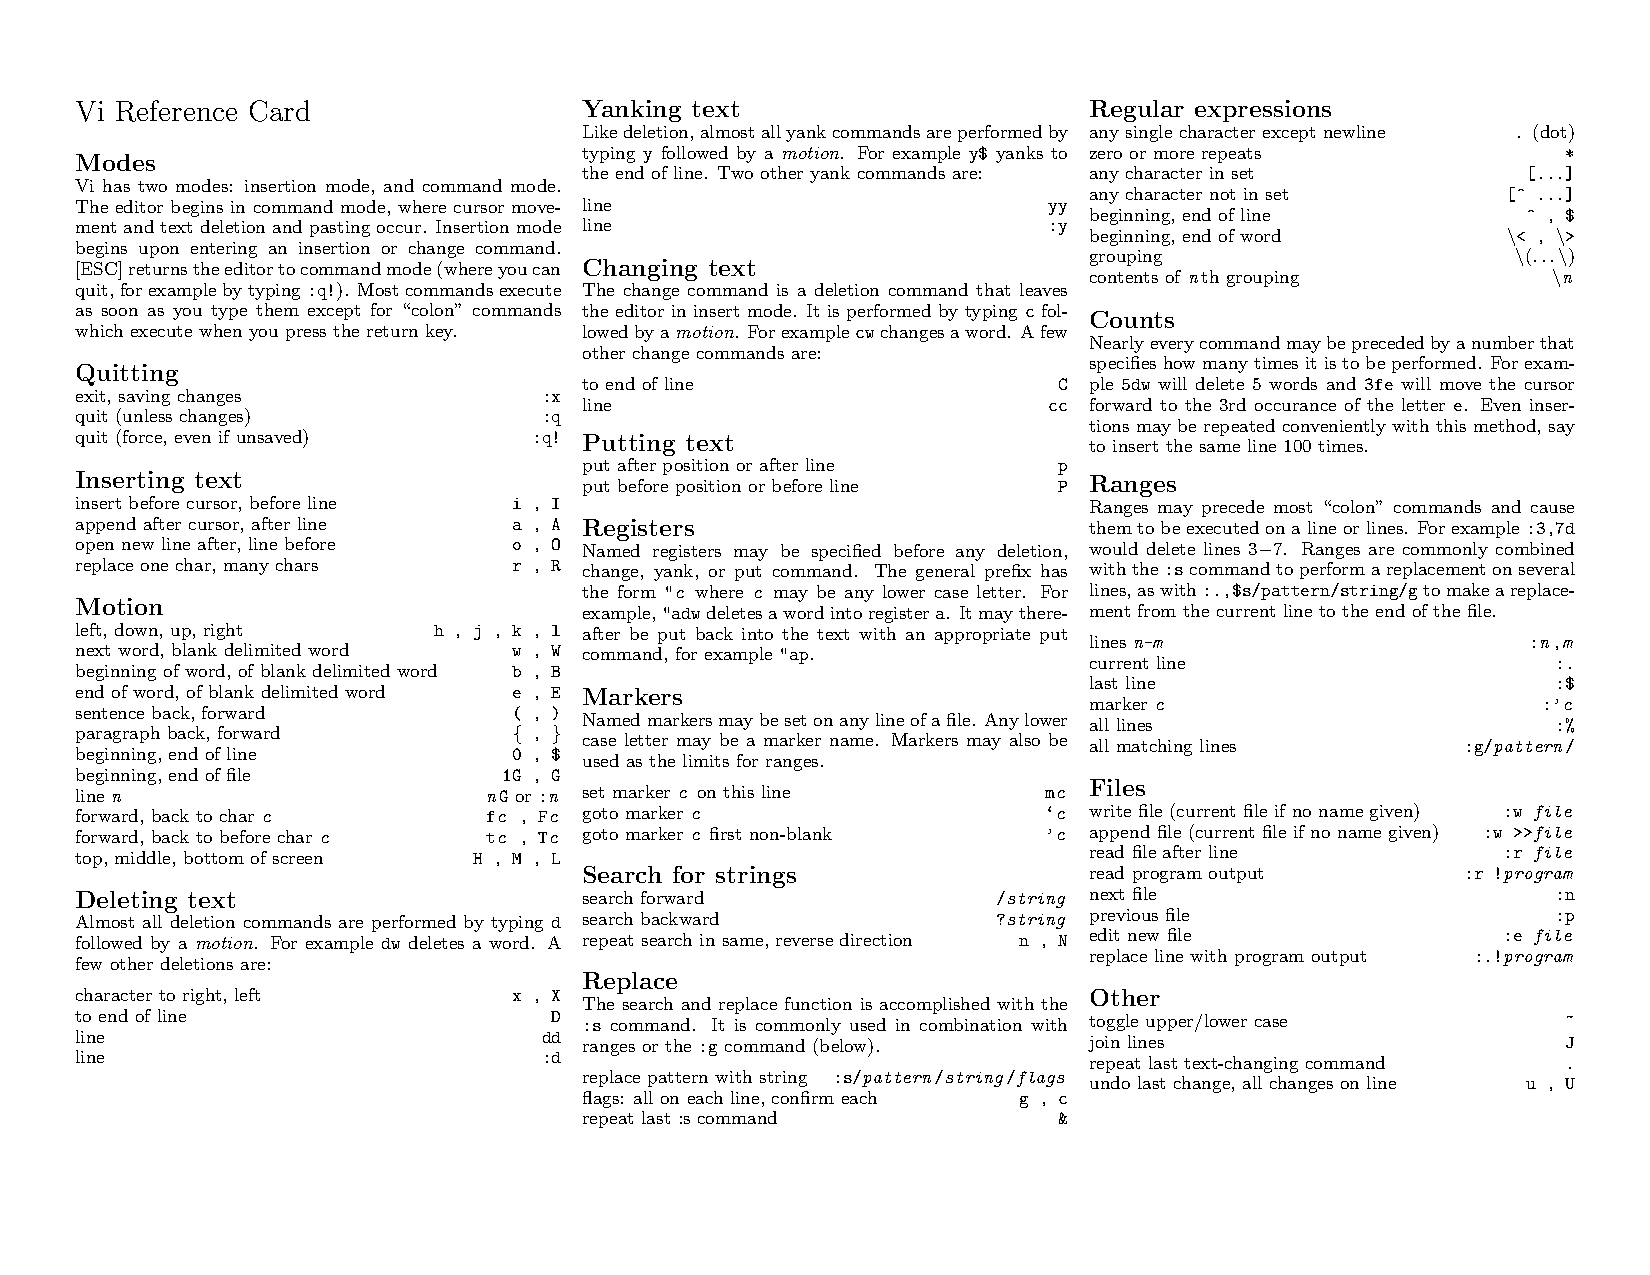
\includepdf[scale=0.95,pages={1},pagecommand={\thispagestyle{fancy}},pagecommand={\thispagestyle{fancy}{\label{subsec:vi}}},lastpage=1,angle=90]{img/viRef.pdf}
}



\begin{example}[Utworzenie i~uruchomienie skryptu] \label{ex:prostakomenda7}


Powłoka, jako interpreter, wykonuje pewien program.  Kolejne komendy programu mogą być wpisywane na bieżąco w~terminalu lub cały program może być dostarczony do powłoki w~postaci skryptu. Należy utworzyć plik o~nazwie \lstinline[style=MyBashStyle]{skrypt} edytorem tekstu \lstinline[style=MyBashStyle]{vi} o~treści:

\begin{lstlisting}[style=MyBashStyle]
date ; ls
\end{lstlisting}

W~następnej kolejności uruchomić skrypt powłoki wydając polecenie:

\begin{lstlisting}[style=MyBashStyle]
# /bin/sh skrypt
\end{lstlisting}

Przykład ilustruje skrypt powłoki. Na ogół skrypty składają się z plików, w których są zapisane komendy, interpretowane przez powłokę. Skrypt można uruchomić wpisując w wiersz poleceń jego nazwę. Jednak bezpośrednie wpisanie jego nazwy kończy się niepowodzeniem:

\begin{lstlisting}[style=MyBashStyle]
# ./skrypt
sh: ./skrypt: cannot execute - Permission denied
\end{lstlisting}

W tej sytuacji należy zapewnić, aby skrypt miał odpowiednie atrybuty oraz upewnić się, że uruchamiany jest właściwy interpreter poleceń. Aby zmienić atrybuty pliku należy użyć następującego polecenia:

\begin{lstlisting}[style=MyBashStyle]
# chmod a+x ./skrypt
\end{lstlisting}

Uruchomić \lstinline[style=MyBashStyle]{skrypt} w~linii poleceń.
\end{example}


\begin{example}[Prosty skrypt powłoki]\label{ex:prostakomenda8}


Należy także uzupełnić plik \lstinline[style=MyBashStyle]{skrypt}, tak, żeby miał postać:

\begin{lstlisting}[style=MyBashStyle]
#!/bin/sh
# wypisz date i wyswietl zawartosc katalogu
date ; ls
\end{lstlisting}

Znak \lstinline[style=MyBashStyle]{#} stanowi znak komentarza w~skrypcie. Wiersze zaczynające się od tego znaku są ignorowane przez interpreter poleceń i~traktowane jako komentarz, oprócz pierwszej linii z~komendą \lstinline[style=MyBashStyle]{#!/bin/sh}. Pierwsza linia kodu przekazuje informacje o~rodzaju powłoki, która powinna wykonać skrypt.
\end{example}


\begin{example}[Prosty skrypt powłoki]\label{ex:prostakomenda9}

Dokumentacja systemu jest dostępna w formie elektronicznej na stronach \href{www.qnx.com}{www.qnx.com}. Skrócony opis interesującego nas polecenia systemowego uzyskujemy poprzez wpisanie w okno terminala polecenia \lstinline[style=MyBashStyle]{use polecenie}, np.:

\begin{lstlisting}[style=MyBashStyle]
# use date
\end{lstlisting}
\end{example}

\subsection{System plików}

W systemie QNX Neutrino prawie wszystkie zasoby są plikami. Dane, urządzenia, bloki pamięci, a nawet pewne usługi są reprezentowane przez abstrakcję plików. Mechanizm plików pozwala na jednolity dostęp do zasobów zarówno lokalnych, jak i~zdalnych, za pomocą poleceń i programów usługowych wydawanych z okienka poleceń. Typowe drzewo plików w~systemie QNX przedstawiono na rysunku~\ref{fig:drzewo}.

\begin{figure}[!h]
\centering
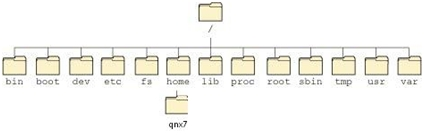
\includegraphics[width=0.75\textwidth]{img/systemplikow}
\caption{Drzewo plików w systemie QNX}
\label{fig:drzewo}
\end{figure}

\begin{myitemize}
\item Katalog główny \lstinline[style=MyBashStyle]{/} jest miejscem montowania twardego dysku lub pamięci flash.
\item \lstinline[style=MyBashStyle]{/bin} - zawiera podstawowe komendy systemowe (np. \lstinline[style=MyBashStyle]{ls}, \lstinline[style=MyBashStyle]{chmod}).
\item \lstinline[style=MyBashStyle]{/boot} - zawiera pliki i katalogi związane z obrazami systemu operacyjnego.
\item \lstinline[style=MyBashStyle]{/dev} - katalog przynależy do menadżera zasobów, w którym przechowywane są informacje o urządzeniach dostępnych w systemie.
\item \lstinline[style=MyBashStyle]{/etc} - zawiera pliki i programy używane do administracji i konfiguracji systemu.
\item \lstinline[style=MyBashStyle]{/fs} - w katalogu są montowane dodatkowe systemy plików.
\item \lstinline[style=MyBashStyle]{/home} - katalogi domowe użytkowników.
\item \lstinline[style=MyBashStyle]{/lib} - zawiera współdzielone biblioteki używane przez inne programy, procesy.
\item \lstinline[style=MyBashStyle]{/proc} - katalog, w którym są zawarte informacje o procesach i przestrzeni nazw.
\item \lstinline[style=MyBashStyle]{/root} - katalog domowy dla użytkownika root.
\item \lstinline[style=MyBashStyle]{/sbin} - zawiera niezbędne pliki wykonywalne (np. sterowniki, programy inicjujące, konfiguracyjne, menadżery).
\item \lstinline[style=MyBashStyle]{/tmp} - zawiera pliki tymczasowe.
\item \lstinline[style=MyBashStyle]{/usr} - zawiera współdzielone dane, tylko do odczytu.
\item \lstinline[style=MyBashStyle]{/var} - zawiera zmienne dane (np. cache, logi).
\end{myitemize}

Bardziej obszerny opis struktury i~hierarchii katalogów w~systemach klasy Unix, do których należy QNX, można znaleźć pod adresem \href{https://en.wikipedia.org/wiki/Unix\_filesystem}{https://en.wikipedia.org/wiki/Unix\_filesystem}. W~systemie QNX występują różne typy plików. Ich zestawienie przedstawiono w~tabeli \ref{tab:typyplikow}.


\begin{table}[h!]
\centering
\caption{Typy plików w~systemie QNX}
\setlength{\arrayrulewidth}{1pt}
\setlength{\tabcolsep}{6pt}
\renewcommand{\arraystretch}{1.2}
\begin{tabular}{ |p{0.15\textwidth}|p{0.3\textwidth}|p{0.4\textwidth}| }
\hline \rowcolor{gray}
\textbf{Oznaczenie} & \textbf{Typ pliku} & \textbf{Opis} \\ \hline
\mbox{\lstinline[style=MyBashStyle]{d}} & Katalog (ang. directory) & Plik zawierający inne pliki i katalogi. \\ \hline
\mbox{\lstinline[style=MyBashStyle]{l}} & Dowiązanie symboliczne (ang. symbolic link) & Dodatkowa nazwa pliku, który jest umieszczony w innym miejscu. \\ \hline
\mbox{\lstinline[style=MyBashStyle]{n}} & Plik specjalny & Np. blok pamięci współdzielonej. \\ \hline
\mbox{\lstinline[style=MyBashStyle]{c}} & Specjalny plik znakowy (ang. charakter device) & Urządzenie z dostępem znakowym (konsola, porty szeregowe, równoległe). \\ \hline
\mbox{\lstinline[style=MyBashStyle]{p}} & Plik specjalny FIFO & Bufor cykliczny w pamięci operacyjnej. \\ \hline
\mbox{\lstinline[style=MyBashStyle]{b}} & Specjalny plik blokowy (ang. block device) & Urządzenie z dostępem blokowym (dysk, partycja dyskowa). \\ \hline
\mbox{\lstinline[style=MyBashStyle]{s}} & Gniazdko (ang. socket)	 & Plik komunikacji sieciowej. \\ \hline
\end{tabular}
\label{tab:typyplikow}
\end{table}


Pliki są zorganizowane w katalogi. Katalogi mają strukturę drzewa z korzeniem \lstinline[style=MyBashStyle]{/} (\lstinline[style=MyBashStyle]{root}). Aby wskazać na konkretny obiekt w systemie plików, należy podać jego ścieżkę. Rozróżniamy ścieżki absolutne i~względne. Ścieżka absolutna zaczyna się od znaku \lstinline[style=MyBashStyle]{/} , np. \lstinline[style=MyBashStyle]{/etc/passwd}. Ścieżka relatywna zaczyna się od znaku innego niż \lstinline[style=MyBashStyle]{/} , np. \lstinline[style=MyBashStyle]{etc/passwd} .


\begin{example}[Wylistowanie zawartości katalogu]\label{ex:wylistowanie}

Pokazać zawartość bieżącego katalogu:

\begin{lstlisting}[style=MyBashStyle]
# ls -l
total 419571
drwxr-xr-x   2 root      root           3072 Feb 23  2014 bin
drwxr-xr-x   4 root      root           1024 Feb 23  2014 boot
dr-xr-xr-x   2 root      root              0 Oct 22 15:07 dev
drwxr-xr-x  10 root      root           3072 Feb 23  2014 etc
drwxr-xr-x   2 root      root           1024 Feb 23  2014 home
drwxr-xr-x   4 root      root           5120 Feb 23  2014 lib
drwxr-xr-x   3 root      root           1024 Feb 23  2014 libexec
dr-xr-xr-x   2 root      root      214798336 Oct 22 15:07 proc
drwxr-xr-x   2 root      root           1024 Sep 30 21:43 root
drwxr-xr-x   2 root      root           3072 Feb 23  2014 sbin
-rw-rw-rw-   1 root      root             11 Oct 22 12:14 skrypt
drwxr-xr-x   2 root      root           1024 Oct 22 12:30 tmp
drwxr-xr-x   7 root      root           1024 Feb 23  2014 usr
drwxr-xr-x   4 root      root           1024 Feb 23  2014 var
\end{lstlisting}

Pokazać zawartość innego katalogu:

\begin{lstlisting}[style=MyBashStyle]
# ls -la /usr/
\end{lstlisting}

Argument \lstinline[style=MyBashStyle]{-l} służy do listowania w formacie tzw. długim, natomiast argument \lstinline[style=MyBashStyle]{-a} do listowania ukrytych plików. Sprawdzić inne parametry polecenia ls następująco:

\begin{lstlisting}[style=MyBashStyle]
# use ls
\end{lstlisting}
\end{example}

\begin{example}[Obejrzenie zawartości pliku]\label{ex:obejrzenie}

Oprócz listowania zawartości katalogów, istotna jest możliwość oglądania zawartości plików (np. skryptowych):

\begin{lstlisting}[style=MyBashStyle]
# cat /skrypt
# cat -n /skrypt			# -n numerowanie linii
# cat -n /etc/passwd
\end{lstlisting}
\end{example}


\begin{example}[Wyświetlanie liczby wierszy, słów i~bajtów zawartych w pliku]\label{ex:wys}

Aby uzyskać informację o całkowitej liczbie linii, słów i~znaków, zawartych w pliku można użyć polecenie \lstinline[style=MyBashStyle]{wc} (ang. word count):

\begin{lstlisting}[style=MyBashStyle]
# wc /skrypt
\end{lstlisting}

Dostępne argumenty polecenia przedstawiono w~tabeli \ref{tab:opcjeWC}.


\begin{table}[h!]
\centering
\caption{Opcje polecenia wc}
\setlength{\arrayrulewidth}{1pt}
\setlength{\tabcolsep}{6pt}
\renewcommand{\arraystretch}{1.2}
\begin{tabular}{ |p{0.15\textwidth}|p{0.4\textwidth}|}
\hline \rowcolor{gray}
\textbf{Argumenty} & \textbf{Opis} \\ \hline
\mbox{\lstinline[style=MyBashStyle]{-l}} & Oblicza liczbę linii \\ \hline
\mbox{\lstinline[style=MyBashStyle]{-w}} & Oblicza liczbę słów \\ \hline
\mbox{\lstinline[style=MyBashStyle]{-m}} & Oblicza liczbę znaków \\ \hline
\mbox{\lstinline[style=MyBashStyle]{-c}} & Oblicza liczbę znaków  \\ \hline
\end{tabular}
\label{tab:opcjeWC}
\end{table}

\begin{example}[Poruszanie się po systemie plików]

System operacyjny jest wyposażony w zestaw instrukcji, które umożliwiają poruszanie się po drzewie plików. Najważniejsze zestawiono w tabeli~\ref{tab:poruszanie} i~zilustrowano w przykładzie.

\begin{table}[h!]
\centering
\caption{Poruszanie się po systemie plików}
\setlength{\arrayrulewidth}{1pt}
\setlength{\tabcolsep}{6pt}
\renewcommand{\arraystretch}{1.2}
\begin{tabular}{ |p{0.15\textwidth}|p{0.4\textwidth}|}
\hline \rowcolor{gray}
\textbf{Polecenie} & \textbf{Opis} \\ \hline
\mbox{\lstinline[style=MyBashStyle]{pwd}} & Wyświetlenie nazwy katalogu bieżącego (ang. print working directory) \\ \hline
\mbox{\lstinline[style=MyBashStyle]{cd}}  & Zmiana katalogu bieżącego (ang. change directory) \\ \hline
\mbox{\lstinline[style=MyBashStyle]{cd..}} & Przejście do katalogu nadrzędnego \\ \hline
\mbox{\lstinline[style=MyBashStyle]{cd /}} & Przejście do katalogu głównego \\ \hline
%\mbox{\lstinline[style=MyBashStyle]{cd ~}} &	Przejście do katalogu domowego \\ \hline
\end{tabular}
\label{tab:poruszanie}
\end{table}
\end{example}



Wprowadzić następujące komendy w~wierszu poleceń.

\begin{lstlisting}[style=MyBashStyle]
# pwd			# Nazwa katalogu biezacego (dla naszego przypadku)
/
# cd /usr			# Przejscie do katalogu uzytkownika
# pwd
/usr
# cd ..			# Przejscie do katalogu nadrzednego
# pwd
/
# ls .			# Wylistowanie nazw plikow w biezacym katalogu
...
# ls -l 			# Wylistowanie ze szczegolami
\end{lstlisting}
\end{example}

\begin{example}[Utworzenie i kasowanie katalogów]

Pliki w systemie plików można tworzyć i usuwać. Katalogi można również modyfikować. Najczęściej używane polecenia służą do tworzenia, kopiowania, przenoszenia oraz usuwania katalogów. Zestawienie podstawowych poleceń podano w tabeli~\ref{tab:tworziusun}.

\begin{table}[h!]
\centering
\caption{Tworzenie i usuwanie katalogów i~plików}
\setlength{\arrayrulewidth}{1pt}
\setlength{\tabcolsep}{6pt}
\renewcommand{\arraystretch}{1.2}
\begin{tabular}{ |p{0.15\textwidth}|p{0.4\textwidth}|}
\hline \rowcolor{gray}
\textbf{Polecenie} & \textbf{Opis} \\ \hline
\mbox{\lstinline[style=MyBashStyle]{touch plik}} & Utworzenie pustego pliku lub zmiana daty modyfikacji istniejącego \\ \hline
\mbox{\lstinline[style=MyBashStyle]{cd}}  & Zmiana katalogu bieżącego (ang. change directory) \\ \hline
\mbox{\lstinline[style=MyBashStyle]{rm [-Rfi] plik}} & Usunięcie pliku: \mbox{\lstinline[style=MyBashStyle]{-i}} - żądanie potwierdzenie; \mbox{\lstinline[style=MyBashStyle]{-f}} - bezwarunkowe kasowanie pliku; \mbox{\lstinline[style=MyBashStyle]{-R}} - kasowanie zawartości katalogu z~podkatalogami  \\ \hline
\mbox{\lstinline[style=MyBashStyle]{mkdir katalog}} & Utworzenie katalogu o nazwie \mbox{\lstinline[style=MyBashStyle]{katalog}} \\ \hline
\mbox{\lstinline[style=MyBashStyle]{rmdir katalog}} &	Usunięcie katalogu o nazwie \mbox{\lstinline[style=MyBashStyle]{katalog}}  \\ \hline
\end{tabular}
\label{tab:tworziusun}
\end{table}

Sprawdzić działanie następujących komend:

\begin{lstlisting}[style=MyBashStyle]
# pwd			# Nazwa katalogu biezacego
/
# cd /home			# Przejdz do katalogu home
# mkdir katalog			# Utworzenie katalogu
# cd katalog			# Przejdz do katalogu
# mkdir podkatalog			# Utworzenie podkatalogu
# touch plik			# Utworzenie pustego pliku
# touch plik2			# Utworzenie pustego pliku
# rm plik2			# Usuniecie pustego pliku
# rmdir podkatalog			# Usuniecie podkatalogu
# cd .. 			# Wyjscie do katalogu nadrzednego
# rmdir katalog 			# Proba usuniecia podkatalogu
katalog/: Directory not empty
# rm -Ri katalog			# Usuniecie rekursywne z potwierdzeniem
rm: remove katalog/plik? (y/N) y
rm: remove directory katalog? (y/N) y
\end{lstlisting}

\end{example}


\begin{example}[Przenoszenie i~kopiowanie katalogów i~plików]

Pliki i~katalogi można kopiować i~przenosić. Zestawienie najważniejszych komend przedstawiono w~tabeli~\ref{tab:przenos}.

\begin{table}[h!]
\centering
\caption{Przenoszenie i~kopiowanie katalogów i~plików}
\setlength{\arrayrulewidth}{1pt}
\setlength{\tabcolsep}{6pt}
\renewcommand{\arraystretch}{1.2}
\begin{tabular}{ |p{0.23\textwidth}|p{0.4\textwidth}|}
\hline \rowcolor{gray}
\textbf{Polecenie} & \textbf{Opis} \\ \hline
\mbox{\lstinline[deletekeywords={if}]{mv [-if] zrodlo cel}} & Przenoszenie lub zmiana nazwy plików: \mbox{\lstinline[style=MyBashStyle]{-i}} - żądanie potwierdzenia, gdy plik docelowy może być nadpisany; \mbox{\lstinline[style=MyBashStyle]{-f}} - bezwarunkowe skopiowanie pliku \\ \hline
\mbox{\lstinline[style=MyBashStyle]{cp [-ifR] zrodlo cel}}  & Kopiowanie plików: \mbox{\lstinline[style=MyBashStyle]{-i}} - żądanie potwierdzenia, gdy plik docelowy może być nadpisany; \mbox{\lstinline[style=MyBashStyle]{-f}} - bezwarunkowe skopiowanie pliku; \mbox{\lstinline[style=MyBashStyle]{-R}} - kopiowanie zawartości katalogu z podkatalogami \\ \hline
\end{tabular}
\label{tab:przenos}
\end{table}

Sprawdzić działanie następujących komend:

\begin{lstlisting}[style=MyBashStyle]
# pwd
/home
# mkdir katalog
# cd katalog
# touch pliczek
# cd ..
# mv ./katalog/pliczek .			# Przeniesienie do katalogu biezacego
# mv pliczek plik.dat			# Zmiana nazwy pliku
# cp plik.dat katalog			# Skopiowanie pliku do katalogu
# cp -Ri katalog katalog2			# Skopiowanie katalogu do katalogu2 razem z zawartoscia
\end{lstlisting}
\end{example}


\begin{example}[Zmiana atrybutów pliku]

Pliki w systemie mają określonych właścicieli, grupy użytkowników, a także zestawy atrybutów do nich przypisanych. System umożliwia dostęp do plików w trybie odczytu, zapisu lub wykonania. Symboliczne oznaczenia praw dostępu do pliku są następujące:

\begin{myitemize}
\item \lstinline[style=MyBashStyle]{r} - prawo odczytu (ang. read)
\item \lstinline[style=MyBashStyle]{w} - prawo zapisu (ang. write)
\item \lstinline[style=MyBashStyle]{x} - prawo wykonania (ang. execute)
\end{myitemize}

Prawa te mogą być zdefiniowane dla właściciela pliku, grupy, do której on należy i wszystkich innych użytkowników.

\begin{myitemize}
\item \lstinline[style=MyBashStyle]{u} - właściciel pliku (ang. user)
\item \lstinline[style=MyBashStyle]{g} - grupa (ang. group)
\item \lstinline[style=MyBashStyle]{o} - inni użytkownicy (ang. other)
\end{myitemize}

Aby obejrzeć właściciela pliku oraz atrybuty wykonajmy następujące polecenie:

\begin{lstlisting}[style=MyBashStyle]
# ls -l /home/plik.dat
-rw-rw-rw- 1 root root 0 Oct 22 11:41 /home/plik.dat
\end{lstlisting}

W~terminalu wyświetlone zostały w~kolejności atrybuty dla właściciela (\lstinline[style=MyBashStyle]{rw-}), grupy (\lstinline[style=MyBashStyle]{rw-}) oraz innych użytkowników (\lstinline[style=MyBashStyle]{rw-}); wskazano także liczbę dowiązań \lstinline[style=MyBashStyle]{1}, nazwę właściciela pliku \lstinline[style=MyBashStyle]{root}, nazwę grupy \lstinline[style=MyBashStyle]{root}, rozmiar pliku \lstinline[style=MyBashStyle]{0}, datę utworzenia \lstinline[style=MyBashStyle]{Oct 22 11:41} oraz nazwę pliku \lstinline[style=MyBashStyle]{home/plik.dat}.


Atrybuty plików oraz ich właścicieli można zmieniać - zobacz tabela \ref{tab:zmien}.

\begin{table}[h!]
\centering
\caption{Tworzenie i usuwanie katalogów i~plików}
\setlength{\arrayrulewidth}{1pt}
\setlength{\tabcolsep}{6pt}
\renewcommand{\arraystretch}{1.2}
\begin{tabular}{ |p{0.15\textwidth}|p{0.4\textwidth}|}
\hline \rowcolor{gray}
\textbf{Polecenie} & \textbf{Opis} \\ \hline
\mbox{\lstinline[style=MyBashStyle]{chmod}} & Zmiana atrybutów dla pliku, bądź katalogu \\ \hline
\mbox{\lstinline[style=MyBashStyle]{chown}} & Zmiana właściciela (lub opcjonalnie grupy) dla pliku, bądź katalogu \\ \hline
\mbox{\lstinline[style=MyBashStyle]{chgrp}}  & Zmiana grupy dla pliku, bądź katalogu \\ \hline
\end{tabular}
\label{tab:zmien}
\end{table}

Zmiana atrybutów pliku odbywa się wg następujące składni:

\begin{lstlisting}[style=MyBashStyle]
# chmod wlasciciel akcja atrybuty
\end{lstlisting}

gdzie \lstinline[style=MyBashStyle]{wlasciciel} jest jednym ze skrótów literowych (\lstinline[style=MyBashStyle]{u}, \lstinline[style=MyBashStyle]{g}, \lstinline[style=MyBashStyle]{o}, bądź \lstinline[style=MyBashStyle]{a} - dla wszystkich użytkowników), atrybuty dotyczą oznaczeń (\lstinline[style=MyBashStyle]{r}, \lstinline[style=MyBashStyle]{w} lub \lstinline[style=MyBashStyle]{x}). Możliwe do wykonania akcje opisano w~tabeli~\ref{tab:zarzadzanie}.

\begin{table}[h!]
\centering
\caption{Zarządzanie prawami dostępu}
\setlength{\arrayrulewidth}{1pt}
\setlength{\tabcolsep}{6pt}
\renewcommand{\arraystretch}{1.2}
\begin{tabular}{ |p{0.15\textwidth}|p{0.4\textwidth}|}
\hline \rowcolor{gray}
\textbf{Polecenie} & \textbf{Opis} \\ \hline
\mbox{\lstinline[style=MyBashStyle]{+}} & Dodanie praw dostępu \\ \hline
\mbox{\lstinline[style=MyBashStyle]{-}} & Usunięcie praw dostępu \\ \hline
\mbox{\lstinline[style=MyBashStyle]{=}}  & Jawne ustawienie praw dostępu \\ \hline
\end{tabular}
\label{tab:zarzadzanie}
\end{table}

Wykonać następującą serię poleceń:

\begin{lstlisting}[style=MyBashStyle]
# pwd
/home
# ls -l
total 4
drwxrwxrwx   2 root      root           1024 Oct 22 11:43 katalog
drwxrwxrwx   2 root      root           1024 Oct 22 11:43 katalog2
-rw-rw-rw-   1 root      root              0 Oct 22 11:41 plik.dat
# chmod a+rwx plik.dat			# Dodanie praw dostepu dla wszystkich
# ls -l plik.dat
-rwxrwxrwx   1 root      root              0 Oct 22 11:41 plik.dat
# chmod go-wx plik.dat			# Odebranie praw dostepu
# ls -l plik.dat
-rwxr--r--    1 root      root              0 Oct 22 11:41 plik.dat
\end{lstlisting}



\end{example}


\subsection{Obsługa procesów}

W systemie QNX każdy program jest uruchamiany jako proces. System zarządza procesami układając je w hierarchię rodzic-potomek. Proces, który uruchamia inny proces, nazywa się macierzystym, a proces uruchomiony - potomnym. Po wydaniu polecenia w konsoli, np. \lstinline[style=MyBashStyle]{ls}, proces powłoki powołuje do życia nowy proces \lstinline[style=MyBashStyle]{ls}. Powłoka jest więc w tej sytuacji procesem macierzystym, a proces \lstinline[style=MyBashStyle]{ls} jest procesem potomnym.


\begin{example}[Proces uruchomiony w~tle]

Procesy mogą być uruchamiane w pierwszym planie (ang. foreground) i w tle (ang. background). Domyślnie, procesy są uruchamiane w pierwszym planie. Strumień wejścia do programu stanowi klawiatura, natomiast wyniki są wyprowadzane na ekran, np.

\begin{lstlisting}[style=MyBashStyle]
# ls
katalog katalog2 plik.dat
\end{lstlisting}

Procesy tła możemy uruchamiać poprzez dodanie znaku (\lstinline[style=MyBashStyle]{&}):

\begin{lstlisting}[style=MyBashStyle]
# ls &
[1] 1011730
# katalog katalog2 plik.dat

[1] + Done	ls
\end{lstlisting}

Po uruchomieniu programu, na ekranie pojawia się nr zadania \lstinline[style=MyBashStyle]{[1]} oraz numer identyfikujący proces PID (ang. process identification number). Po wciśnięciu klawisza Enter, program kończy zadanie, a~powłoka wyświetla znak zachęty.
Proces uruchomiony w pierwszym planie można przesunąć do tła (bez podłączenia do klawiatury) i na odwrót. Podstawowe komendy, służące kontrolowaniu zadań zestawiono w~tabeli \ref{tab:kontrola2}.

\begin{table}[h!]
\centering
\caption{Kontrola zadań}
\setlength{\arrayrulewidth}{1pt}
\setlength{\tabcolsep}{6pt}
\renewcommand{\arraystretch}{1.2}
\begin{tabular}{ |p{0.15\textwidth}|p{0.4\textwidth}|}
\hline \rowcolor{gray}
\textbf{Polecenie} & \textbf{Opis} \\ \hline
\mbox{\lstinline[style=MyBashStyle]{polecenie &}} & Uruchomienie zadania w tle \\ \hline
\mbox{\lstinline[style=MyBashStyle]{jobs [-l]}} & Listowanie zadań pracujących w tle \\ \hline
\mbox{\lstinline[style=MyBashStyle]{Ctrl+Z}}  & Wstrzymanie bieżącego zadania \\ \hline
\mbox{\lstinline[style=MyBashStyle]{Ctrl+C}}  & Zakończenie bieżącego zadania \\ \hline
\mbox{\lstinline[style=MyBashStyle]{fg [PID]}}  & Przeniesienie procesu działającego w tle na pierwszy plan na podstawie numeru procesu\\ \hline
\mbox{\lstinline[style=MyBashStyle]{fg [jobID]}}  & Przeniesienie procesu działającego w tle na pierwszy plan na podstawie numeru zadania\\ \hline
\mbox{\lstinline[style=MyBashStyle]{bg [PID]}}  & Uruchomienie w tle wstrzymanego zadania na podstawie numeru procesu \\ \hline
\mbox{\lstinline[style=MyBashStyle]{bg [jobID]}}  & Uruchomienie w tle wstrzymanego zadania na podstawie numeru zadania \\ \hline
\end{tabular}
\label{tab:kontrola2}
\end{table}
\end{example}


\begin{example}[Procesy tła i~procesy pierwszoplanowe]

Proces \lstinline[style=MyBashStyle]{top} wyświetla statystyki wydajności systemu operacyjnego. Uruchomić proces \lstinline[style=MyBashStyle]{top} w~pierwszym planie, a~następnie nacisnąć kombinację \mbox{\lstinline[style=MyBashStyle]{Ctrl+Z}}, aby wstrzymać bieżący proces.

\begin{lstlisting}[style=MyBashStyle]
# top
22 processes; 64 threads;
CPU states: 99.9% idle, 0.0% user, 0.0% kernel
Memory: 0 total, 204M avail, page size 4K

      PID   TID PRI STATE    HH:MM:SS    CPU  COMMAND
  1040402     1  10 Rply      0:00:00   0.01% top
     4110     2  21 Rcv       0:00:01   0.00% io-pkt-v4-hc
     4106     1  10 Rcv       0:00:00   0.00% devc-con-hid
     4101     1  10 Rcv       0:00:00   0.00% pci-bios
     4102     2  21 Rcv       0:00:00   0.00% devb-eide
        1     9  10 Rcv       0:00:00   0.00% kernel
...

             Min        Max       Average
CPU idle:     99%        99%        99%
Mem Avail:   204MB      204MB      204MB
Processes:    22         22         22
Threads:      64         64         64

[1] + Stopped top 			# Po wcisnieciu Ctrl+Z
# jobs -l
[1] + 1040402 Stopped top
# fg %1			# Przeniesienie procesy na pierwszy plan; alternatywnie fg 1040402
22 processes; 64 threads;
CPU states: 99.9% idle, 0.0% user, 0.0% kernel
Memory: 0 total, 204M avail, page size 4K

      PID   TID PRI STATE    HH:MM:SS    CPU  COMMAND
  1040402     1  10 Rply      0:00:00   0.01% top
     4110     2  21 Rcv       0:00:01   0.00% io-pkt-v4-hc
 ...

[1] + Stopped top 			# Po wcisnieciu Ctrl+Z
# bg %1 			# Przeniesienie do tla
# jobs -l
[1] + 1040402 Running top
# fg %1 			# Przeniesienie do pierwszego planu
# 			# Po wcisnieciu Ctrl+C
\end{lstlisting}

\end{example}


\begin{example}[Procesy tła i~procesy pierwszoplanowe]

Uruchamiając i testując programy często zachodzi potrzeba zbierania informacji o stanie systemu. Statystyki dostarczają specjalizowane programy, których przegląd umieszczono w tabeli~\ref{tab:statystyki}.

\begin{table}[h!]
\centering
\caption{Statystyki stanu systemu}
\setlength{\arrayrulewidth}{1pt}
\setlength{\tabcolsep}{6pt}
\renewcommand{\arraystretch}{1.2}
\begin{tabular}{ |p{0.15\textwidth}|p{0.4\textwidth}|}
\hline \rowcolor{gray}
\textbf{Polecenie} & \textbf{Opis} \\ \hline
\mbox{\lstinline[style=MyBashStyle]{ps [-f]}} & Wyświetla listę procesów i ich status \\ \hline
\mbox{\lstinline[style=MyBashStyle]{top}} & Wyświetla statystyki wydajnościowe sytemu \\ \hline
\mbox{\lstinline[style=MyBashStyle]{pidin}}  & Wyświetla statystyki systemowe \\ \hline
\mbox{\lstinline[style=MyBashStyle]{hogs}}  & Wyświetla listę procesów, wg użycia procesora \\ \hline
\mbox{\lstinline[style=MyBashStyle]{showmem [-S]}}  & Wyświetla informacje nt. użytej pamięci \\ \hline
\end{tabular}
\label{tab:statystyki}
\end{table}

Obejrzeć tablicę procesów wywołując następujące polecenie:
\begin{lstlisting}[style=MyBashStyle,deletekeywords={ps}]
# ps -f
  UID        PID       PPID  C STIME TTY          TIME CMD
    0      45068          1  - Oct22 ?        00:00:00 inetd
    0       4109          1  - Oct22 ?        00:00:00 sh
    0    1118226       4119  - 17:29 ?        00:00:00 ps -f
    0       4116          1  - Oct22 ?        00:00:00 sh
    0       4118          1  - Oct22 ?        00:00:00 sh
    0       4119          1  - Oct22 ?        00:00:00 sh
\end{lstlisting}

Znaczenie kolumn po wydaniu polecenie \lstinline[style=MyBashStyle]{ps -f} opisano w~tabeli~\ref{tab:opispol}.

\begin{table}[h!]
\centering
\caption{Opis pól wyświetlany przez polecenie ps}
\setlength{\arrayrulewidth}{1pt}
\setlength{\tabcolsep}{6pt}
\renewcommand{\arraystretch}{1.2}
\begin{tabular}{ |p{0.15\textwidth}|p{0.4\textwidth}|}
\hline \rowcolor{gray}
\textbf{Oznaczenie} & \textbf{Opis} \\ \hline
\mbox{\lstinline[style=MyBashStyle]{UID}} & Numer identyfikacyjny użytkownika, który uruchomił proces \\ \hline
\mbox{\lstinline[style=MyBashStyle]{PID}} & Numer identyfikacyjny procesu (potomnego) \\ \hline
\mbox{\lstinline[style=MyBashStyle]{PPID}}  & Numer identyfikacyjny procesu nadrzędnego (macierzystego) \\ \hline
\mbox{\lstinline[style=MyBashStyle]{C}}  & Wykorzystanie procesora \\ \hline
\mbox{\lstinline[style=MyBashStyle]{STIME}}  & Czas uruchomienia procesu \\ \hline
\mbox{\lstinline[style=MyBashStyle]{TTY}}  & Nazwa terminala kontrolującego (niewspierana) \\ \hline
\mbox{\lstinline[style=MyBashStyle]{TIME}}  & Czas działania procesu \\ \hline
\mbox{\lstinline[style=MyBashStyle]{CMD}}  & Komenda, która uruchomiła proces \\ \hline
\end{tabular}
\label{tab:opispol}
\end{table}

Wylistować zawartość statystyk systemowych za pomocą polecenia \lstinline[style=MyBashStyle]{pidin}, \lstinline[style=MyBashStyle]{hogs} oraz \lstinline[style=MyBashStyle]{showmem}.

\begin{lstlisting}[style=MyBashStyle,deletekeywords={ps}]
# pidin | more
...
# hogs
...
# showmem -S
...
\end{lstlisting}

\end{example}


\begin{example}[Usuwanie procesów] Ważną grupą poleceń są komendy umożliwiające przerwanie działania procesów, bądź przesłanie im sygnału. Ich zestawienie przedstawiono w~tabeli \ref{tab:usuwanie}.

\begin{table}[h!]
\centering
\caption{Usuwanie procesów}
\setlength{\arrayrulewidth}{1pt}
\setlength{\tabcolsep}{6pt}
\renewcommand{\arraystretch}{1.2}
\begin{tabular}{ |p{0.45\textwidth}|p{0.4\textwidth}|}
\hline \rowcolor{gray}
\textbf{Polecenie} & \textbf{Opis} \\ \hline
\mbox{\lstinline[style=MyBashStyle]{kill [-nazwa_sygnalu| -nr_sygnalu] PID}} & Przesłanie sygnału do procesu o nr \mbox{\lstinline[style=MyBashStyle]{PID}} \\ \hline
\mbox{\lstinline[style=MyBashStyle]{slay [-nazwa_sygnalu| -nr_sygnalu] pro}} & Przesłanie sygnału do procesu o~nazwie \mbox{\lstinline[style=MyBashStyle]{pro}} \\ \hline
\end{tabular}
\label{tab:usuwanie}
\end{table}

Na działający proces można oddziaływać wysyłając do niego sygnały. Sygnały zostały stworzone z~myślą o sytuacjach wyjątkowych, np. awariach systemu, czy błędach w pracy programu. Mechanizm sygnałów - ideą przypomina mechanizm przerwań. Proces po otrzymaniu sygnału może wykonać pewną procedurę, lub pozostawić obsługę sygnału systemowi. Nazwy sygnałów i ich liczbowe odpowiedniki możemy podejrzeć poleceniem (\lstinline[style=MyBashStyle]{kill -l}). Trzy często używane sygnały przedstawiono w tabeli~\ref{tab:wybranesygnaly}.

\begin{table}[h!]
\centering
\caption{Usuwanie procesów}
\setlength{\arrayrulewidth}{1pt}
\setlength{\tabcolsep}{6pt}
\renewcommand{\arraystretch}{1.2}
\begin{tabular}{ |p{0.1\textwidth}|p{0.1\textwidth}|p{0.4\textwidth}|}
\hline \rowcolor{gray}
\textbf{Nazwa sygnału} & \textbf{Numer sygnału} & \textbf{Opis} \\ \hline
\mbox{\lstinline[style=MyBashStyle]{INT}} & \mbox{\lstinline[style=MyBashStyle]{2}} &  Przerwanie z klawiatury \\ \hline
\mbox{\lstinline[style=MyBashStyle]{KILL}} & \mbox{\lstinline[style=MyBashStyle]{9}} &  Żądanie natychmiastowego zakończenia procesu \\ \hline
\mbox{\lstinline[style=MyBashStyle]{TERM}} & \mbox{\lstinline[style=MyBashStyle]{15}} &  Żądanie normalnego zakończenia procesu \\ \hline
\end{tabular}
\label{tab:wybranesygnaly}
\end{table}


W poniższym przykładzie powołuje się do życia proces \lstinline[style=MyBashStyle]{cat}, a~następnie przesyła się do niego sygnał \lstinline[style=MyBashStyle]{KILL}. Przykład ten wymaga użycia dwóch konsol. Przełączenia pomiędzy konsolami dokonujemy kombinacją klawiszy \lstinline[style=MyBashStyle]{Ctrl+Alt+1} oraz \lstinline[style=MyBashStyle]{Ctrl+Alt+2}.

\begin{lstlisting}[style=MyBashStyle,caption=Konsola 1]
# cat
Terminated
#
\end{lstlisting}

\begin{lstlisting}[style=MyBashStyle,caption=Konsola 2,deletekeywords={cat,ps}]
# ps -f
  UID        PID       PPID  C STIME TTY          TIME CMD
    0      45068          1  - Oct23 ?        00:00:00 inetd
    0       4109          1  - Oct23 ?        00:00:00 sh
    0       4110          1  - Oct23 ?        00:00:00 sh
    0       4111          1  - Oct23 ?        00:00:00 sh
    0       4112          1  - Oct23 ?        00:00:00 sh
    0      81943       4112  - Oct23 ?        00:00:00 cat
    0     110616       4109  - 14:58 ?        00:00:00 ps -f
# kill -TERM 81943
\end{lstlisting}

\end{example}



\subsection{Zmienne}

Zmienne środowiskowe tworzą tzw. środowisko, w którym wykonują się polecenia. Każde polecenie uruchomione w systemie działa w pewnym ,,otoczeniu'' zmiennych środowiskowych. Zmienne pozwalają na przechowywanie wartości, bądź zdefiniowanych przez użytkownika, bądź danych systemowych (zmienne środowiskowe). Powłoka umożliwia tworzenie zmiennych, przypisywanie wartości i modyfikacje oraz ich usuwanie. Podstawowe operacje na zmiennych przedstawiono w tabeli~\ref{tab:operacje}.

\begin{table}[h!]
\centering
\caption{Podstawowe operacje na zmiennych środowiskowych}
\setlength{\arrayrulewidth}{1pt}
\setlength{\tabcolsep}{6pt}
\renewcommand{\arraystretch}{1.2}
\begin{tabular}{ |p{0.3\textwidth}|p{0.4\textwidth}|}
\hline \rowcolor{gray}
\textbf{Polecenie} & \textbf{Opis} \\ \hline
\mbox{\lstinline[style=MyBashStyle]{ZMIENNA=wartosc}} & Przypisanie wartości do \mbox{\lstinline[style=MyBashStyle]{ZMIENNA}}. Jeśli zmienna nie istnieje, to jest tworzona \\ \hline
\mbox{\lstinline[style=MyBashStyle]{$ZMIENNA}} & Użycie wartości zmiennej (substytucja) \\ \hline
\mbox{\lstinline[style=MyBashStyle]{set}}  & Umożliwia m.in. wyświetlenie wszystkich zmiennych \\ \hline
\mbox{\lstinline[style=MyBashStyle]{unset ZMIENNA}}  & Usuwa zmienną \mbox{\lstinline[style=MyBashStyle]{ZMIENNA}} z pamięci (ze środowiska) \\ \hline
\mbox{\lstinline[deletekeywords={export}]{export ZMIENNA[=wartosc]}}  & Powoduje, że \mbox{\lstinline[style=MyBashStyle]{ZMIENNA}} jest przekazywana do środowiska każdego uruchamianego polecenia \\ \hline
\end{tabular}
\label{tab:operacje}
\end{table}

\begin{example}[Podstawowe operacje na zmiennych] Należy przetestować działanie poniższych poleceń.

\begin{lstlisting}[style=MyBashStyle]
# A="foo"
# echo $A
foo
# unset A
# echo $A

# set
...
# echo $PATH
/proc/boot:/bin:/usr/bin:/sbin:/usr/sbin
#
\end{lstlisting}


\end{example}


\begin{example}[Zmienne i~polecenia] Należy przetestować działanie poniższych poleceń.

\begin{lstlisting}[style=MyBashStyle]
# A=1 echo "Zmienna A: " $A
Zmienna A:
# B=2
# echo "Zmienna B: " $B
Zmienna B: 2
#
\end{lstlisting}

Polecenia są wykonywane w swoim własnym środowisku. Środowisko to jest zainicjalizowane niektórymi wartościami otrzymanymi od środowiska macierzystego. Aby zmienna \lstinline[style=MyBashStyle]{A} przenosiła się do środowiska uruchamianych poleceń, należy na niej wykonać polecenie \lstinline[deletekeywords={export}]{export A}. W powyższym przykładzie wartość zmiennej \lstinline[style=MyBashStyle]{A} nie została wyświetlona, ponieważ jest ona definiowana tylko dla środowiska polecenia \lstinline[style=MyBashStyle]{echo}, a podstawienia wartości \lstinline[style=MyBashStyle]{$A} dokonuje wcześniej powłoka. Zmienna \lstinline[style=MyBashStyle]{B} natomiast jest zdefiniowana w~środowisku powłoki, zatem jej wartość \lstinline[style=MyBashStyle]{$B} jest znana w chwili wywołania \lstinline[style=MyBashStyle]{echo}.

\end{example}


\begin{example}[Wyświetlanie kodu zakończenia]
Kod zakończenia ostatnio wykonanego polecenia zapamiętywany jest w specjalnej zmiennej \lstinline[style=MyBashStyle]{$?}. Wyświetl wartość tej zmiennej po wywołaniu polecenia, które zakończyło się sukcesem oraz po zakończeniu polecenia, które nie mogło się powieść.

\begin{lstlisting}[style=MyBashStyle]
# echo "dobre polecenie"
dobre polecenie
# echo $?
0
# zlepolecenie
sh: zlepolecenie: cannot execute - No such file or directory
# echo $?
126
\end{lstlisting}
\end{example}


\begin{example}[Skrypt i~zmienne środowiskowe]
Skrypty po uruchomieniu działają w swoim własnym środowisku. Niektóre zmienne ze środowiska macierzystego (np. ze środowiska powłoki \lstinline[style=MyBashStyle]{sh}) są kopiowane do środowiska skryptu, inne nie. Poniższy przykład ilustruje oddziaływanie między skryptem a jego środowiskiem oraz środowiskiem macierzystym.

Przejść do katalogu \lstinline[style=MyBashStyle]{/home} i~napisać skrypt \lstinline[style=MyBashStyle]{piszA} o~treści:

\begin{lstlisting}[style=MyBashStyle,deletekeywords={echo}]
echo "Zmienna A: " $A
\end{lstlisting}

W terminalu powłoki przeprowadź następujące eksperymenty:

\begin{lstlisting}[style=MyBashStyle,deletekeywords={echo}]
# unset A
# sh piszA
Zmienna A:

# A=10
# sh piszA
Zmienna A:

# A=10 sh piszA
Zmienna A: 10

# export A=20
# sh piszA
Zmienna A: 20
\end{lstlisting}

\end{example}

\subsection{Przetwarzanie tekstu}

Powłoka zawiera specjalne skrypty, które służą do wyświetlania, modyfikacji i formatowania tekstów. Podstawowe komendy zestawiono w tabeli~\ref{tab:wyswietl}.

\begin{table}[h!]
\centering
\caption{Wyświetlanie tekstu}
\setlength{\arrayrulewidth}{1pt}
\setlength{\tabcolsep}{6pt}
\renewcommand{\arraystretch}{1.2}
\begin{tabular}{ |p{0.3\textwidth}|p{0.4\textwidth}|}
\hline \rowcolor{gray}
\textbf{Polecenie} & \textbf{Opis} \\ \hline
\mbox{\lstinline[style=MyBashStyle]{cat [plik]}} & Wyświetlanie całej treści pliku (lub standardowego wejścia) \\ \hline
\mbox{\lstinline[style=MyBashStyle]{more}} & Wyświetlanie ze stronicowaniem \\ \hline
\mbox{\lstinline[style=MyBashStyle]{less}} & Wyświetlanie ze stronicowaniem \\ \hline
\mbox{\lstinline[style=MyBashStyle]{head [-liczbalinii] [plik]}}  & Wyświetlenie kilku pierwszych wierszy tekstu \\ \hline
\mbox{\lstinline[style=MyBashStyle]{tail [-liczbalinii] [plik]}}  & Wyświetlenie kilku ostatnich wierszy tekstu \\ \hline
\end{tabular}
\label{tab:wyswietl}
\end{table}

Jednocześnie możliwe jest filtrowanie tekstu za pomocą poleceń zaprezentowanych w~tabeli~\ref{tab:filtruj}.

\begin{table}[h!]
\centering
\caption{Filtrowanie tekstu}
\setlength{\arrayrulewidth}{1pt}
\setlength{\tabcolsep}{6pt}
\renewcommand{\arraystretch}{1.2}
\begin{tabular}{ |p{0.25\textwidth}|p{0.4\textwidth}|}
\hline \rowcolor{gray}
\textbf{Polecenie} & \textbf{Opis} \\ \hline
\mbox{\lstinline[style=MyBashStyle]{grep wzor [plik]}} & Wyświetlanie tylko linii tekstu pasujących do wzorca \\ \hline
\mbox{\lstinline[style=MyBashStyle]{sort [plik]}} & Wyświetlanie posortowanej treści \\ \hline
\mbox{\lstinline[style=MyBashStyle]{wc [plik]}} & Zliczanie wierszy, słów, znaków, itp. \\ \hline
\end{tabular}
\label{tab:filtruj}
\end{table}

\subsection{Strumienie wejściowo-wyjściowe}

Uruchomiony program ma do dyspozycji trzy strumienie danych. Każdy z tych plików jest reprezentowany przez małą liczbę całkowitą, zwaną deskryptorem pliku (uchwytem do pliku) - patrz tabela~\ref{tab:strumienie}.

\begin{table}[h!]
\centering
\caption{Strumienie wejście-wyjście}
\setlength{\arrayrulewidth}{1pt}
\setlength{\tabcolsep}{6pt}
\renewcommand{\arraystretch}{1.2}
\begin{tabular}{ |p{0.15\textwidth}|p{0.15\textwidth}|p{0.4\textwidth}|}
\hline \rowcolor{gray}
\textbf{Strumień} & \textbf{Deskryptor} & \textbf{Opis} \\ \hline
\mbox{\lstinline[style=MyBashStyle]{stdin}} & \mbox{\lstinline[style=MyBashStyle]{0}} &  Standardowy strumień wejściowy  \\ \hline
\mbox{\lstinline[style=MyBashStyle]{stdout}} & \mbox{\lstinline[style=MyBashStyle]{1}} &  Standardowy strumień wyjściowy  \\ \hline
\mbox{\lstinline[style=MyBashStyle]{stderr}} & \mbox{\lstinline[style=MyBashStyle]{2}} &  Standardowy strumień dla komunikatów o~błędach  \\ \hline
\end{tabular}
\label{tab:strumienie}
\end{table}

Wiele programów działa w ten sposób, że pobierają tekst ze strumienia \lstinline[style=MyBashStyle]{stdin}, przetwarzają go wysyłając rezultat do strumienia \lstinline[style=MyBashStyle]{stdout}, a komunikaty o błędach do \lstinline[style=MyBashStyle]{stderr}, tak, jak przedstawiono to na rysunku~\ref{fig:strumienie}. Przy zwykłym uruchomieniu programu, strumień \lstinline[style=MyBashStyle]{stdin} przychodzi z klawiatury a strumienie \lstinline[style=MyBashStyle]{stdout} i \lstinline[style=MyBashStyle]{stderr} są wyświetlane w~konsoli.

\begin{figure}[!h]
\centering
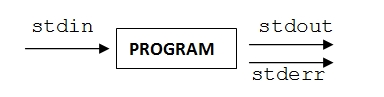
\includegraphics[width=0.5\textwidth]{img/strumienie}
\caption{Strumienie wejście-wyjście}
\label{fig:strumienie}
\end{figure}

Źródło oraz wyjście danych można zmienić stosując tzw. przekierowanie strumieni. Jako strumień wejściowy do programu można wysłać zawartość pliku. Służy do tego zapis:

\begin{lstlisting}[style=MyBashStyle]
# polecenie < plik
\end{lstlisting}


\begin{example}[Przekierowanie strumienia wejściowego]

Polecenie \lstinline[style=MyBashStyle]{cat} wywołane bez żadnych argumentów kopiuje strumień \lstinline[style=MyBashStyle]{stdin} do strumienia \lstinline[style=MyBashStyle]{stdout}. Podaj zawartość pliku \lstinline[style=MyBashStyle]{piszA} jako strumień wejściowy do polecenia \lstinline[style=MyBashStyle]{cat}.

\begin{lstlisting}[style=MyBashStyle]
# cat < piszA
\end{lstlisting}

Strumień wyjściowy \lstinline[style=MyBashStyle]{stdout} możemy przekierować do pliku za pomocą zapisu:

\begin{lstlisting}[style=MyBashStyle]
# cat > mojplik
pierwszy wiersz
drugi wiersz
trzeci wiersz
#                          # Ctrl+C
# cat mojplik
\end{lstlisting}

W ten sposób wyjście z programu zostanie zapisane do pliku \lstinline[style=MyBashStyle]{plik}. Można również sprawić, aby wyjście zostało dopisane do pliku:

\begin{lstlisting}[style=MyBashStyle]
# cat >> mojplik
czwarty wiersz
piaty wiersz
#                          # Ctrl+C
# cat mojplik
\end{lstlisting}
\end{example}


\begin{example}[Przekierowanie strumienia wyjściowego]

Wylistuj zawartość bieżącego katalogu i~przekieruj listing do pliku \lstinline[style=MyBashStyle]{mojplik2}. Wyświetl zawartość pliku \lstinline[style=MyBashStyle]{mojplik2}.


\begin{lstlisting}[style=MyBashStyle]
# ls -la > mojplik2
# cat mojplik2
\end{lstlisting}

Wyjście \lstinline[style=MyBashStyle]{stderr} można przekierować do pliku w następujący sposób:

\begin{lstlisting}[style=MyBashStyle]
# polecenie 2> plikzbledem
# cat plikzbledem
\end{lstlisting}

lub

\begin{lstlisting}[style=MyBashStyle]
# polecenie 2>> plikzbledem
# cat plikzbledem
\end{lstlisting}
\end{example}

\begin{example}[Przekierowanie strumienia stderr]

Próba skopiowania nieistniejącego pliku spowoduje wyświetlenie komunikatu o błędzie. Przekieruj ten komunikat do pliku \lstinline[style=MyBashStyle]{plikzbledem2} po czym wyświetl zawartość pliku

\begin{lstlisting}[style=MyBashStyle]
# cp pliknieist . 2> plikzbledem2
# cat plikzbledem2
\end{lstlisting}
\end{example}

\begin{example}[Jednoczesne przekierowanie strumienia stdin i stdout]
Podaj zawartość pliku \lstinline[style=MyBashStyle]{piszA} na wejście polecenia \lstinline[style=MyBashStyle]{cat} a wyjście przekieruj do pliku wyjscie. Wyświetl zawartość pliku \lstinline[style=MyBashStyle]{wyjscie}.

\begin{lstlisting}[style=MyBashStyle]
# cat < piszA > wyjscie
# cat wyjscie
\end{lstlisting}
\end{example}

\begin{example}[Potoki i~filtrowanie wyników]
Polecenia można łączyć w potoki (ang. pipes). Dokonuje się tego poprzez zapis:

\begin{lstlisting}[style=MyBashStyle]
# polecenie1 | polecenie 2 | ...
\end{lstlisting}

\begin{figure}[!h]
\centering
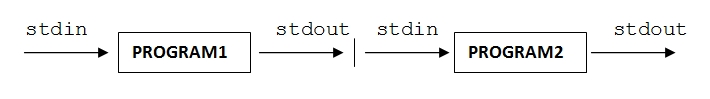
\includegraphics[width=1.0\textwidth]{img/potoki}
\caption{Zasada działania potoków (pipes)}
\label{fig:potoki}
\end{figure}

Wyjście \lstinline[style=MyBashStyle]{stdout} programu1 jest podawane na wejście \lstinline[style=MyBashStyle]{stdin} programu2 itd. Kodem zakończenia potoku jest kod zwrócony przez ostatnie polecenie.

Polecenie \lstinline[style=MyBashStyle]{grep} filtruje przychodzący tekst przepuszczając tylko linie tekstu pasujące do wzorca. Należy ,,przepompować'' zawartość pliku \lstinline[style=MyBashStyle]{piszA} poleceniem \lstinline[style=MyBashStyle]{cat} do polecenia \lstinline[style=MyBashStyle]{grep}, aby wyszukać linie zawierające literę \lstinline[style=MyBashStyle]{A}.

\begin{lstlisting}[style=MyBashStyle]
# cat piszA | grep 'A'
\end{lstlisting}

\end{example}

\begin{example}[Sortowanie i obcinanie wyników]

Wyświetl listę pięciu największych plików w bieżącym katalogu:

\begin{lstlisting}[style=MyBashStyle]
# ls -s | sort -n | tail -5
\end{lstlisting}
\end{example}

\begin{example}[Prosta sekwencja poleceń]

Polecenia można grupować w tzw. sekwencje. Służą do tego operatory \lstinline[style=MyBashStyle]{;}, \lstinline[style=MyBashStyle]{&&} i~\lstinline[style=MyBashStyle]{||}. Polecenia połączone operatorem \lstinline[style=MyBashStyle]{;} wykonują się jedno po drugim bezwarunkowo.

W jednej linii zdefiniuj zmienną o nazwie \lstinline[style=MyBashStyle]{FOO} i~wyświetl jej zawartość.

\begin{lstlisting}[style=MyBashStyle]
# FOO='To jest zmienna FOO';echo $FOO
\end{lstlisting}

\end{example}

\begin{example}[Sekwencja warunkowa - koniunkcja]
Operator \lstinline[style=MyBashStyle]{&&} umożliwia wykonanie następnego polecenia w sekwencji tylko, jeśli poprzednie wykonało się pomyślnie (kod wykonania \lstinline[style=MyBashStyle]{=0}). Polecenie \lstinline[style=MyBashStyle]{grep} zwraca \lstinline[style=MyBashStyle]{0} (sukces), jeśli poszukiwany wzór występuje w tekście. W przeciwnym przypadku zwraca wartość niezerową (błąd). Przeszukać zawartość pliku \lstinline[style=MyBashStyle]{piszA} w poszukiwaniu wzorca \lstinline[style=MyBashStyle]{A} i wyświetlić napis "Znaleziono", jeśli wzorzec wystąpił. Wykonać podobny zabieg dla wzorca \lstinline[style=MyBashStyle]{kawa}.

\begin{lstlisting}[style=MyBashStyle]
# cat piszA | grep 'A' && echo "Znaleziono"
Znaleziono
# echo $?
0
# cat piszA | grep 'kawa' && echo "Znaleziono"
# echo $?
1
\end{lstlisting}
\end{example}

\begin{example}[Sekwencja warunkowa - alternatywa]
Powtórzyć poprzedni przykład używając operatora \lstinline[style=MyBashStyle]{||}, zamiast \lstinline[style=MyBashStyle]{&&}.
\begin{lstlisting}[style=MyBashStyle]
# cat piszA | grep 'A' || echo "Nie znaleziono"
echo "Zmienna A: " $A
# echo $?
0
# cat piszA | grep 'kawa' || echo "Nie znaleziono"
Nie znaleziono
# echo $?
0
\end{lstlisting}
\end{example}

\subsection{Ćwiczenia}

\begin{myenumerate}
\item W systemie pomocy znajdź opis programu do archiwizacji danych tar. Spakować wszystkie pliki znajdujące się w katalogu bieżącym (tj. \lstinline[style=MyBashStyle]{/home}) do pojedynczego archiwum o nazwie \lstinline[style=MyBashStyle]{programy.tar} (opcje \lstinline[style=MyBashStyle]{-cvf}). Utworzyć w katalogu domowym, katalog o nazwie \lstinline[style=MyBashStyle]{Dokumenty}. Skopiować archiwum do katalogu \lstinline[style=MyBashStyle]{/home/Dokumenty} i~tam go rozpakować (opcje \lstinline[style=MyBashStyle]{-xvf}).
\end{myenumerate}

\cleardoublepage

\section{Wprowadzenie do QNX Momentics}


W celu opracowania programów pracujących pod kontrolą systemu operacyjnego czasu rzeczywistego (hard real time), będziemy potrzebowali Platformy Programistycznej QNX. W jej skład wchodzi pakiet QNX Momentics Tool Suite, składający się z elementów niezbędnych do rozwoju i uruchomienia oprogramowania pod QNX Neutrino - patrz rysunek~\ref{fig:qnxMomentics}. Do tej grupy należą kompilatory, linker, biblioteki i~inne komponenty systemu operacyjnego, zbudowane dla wszystkich architektur wspieranych przez QNX Neutrino. Posługując się QNX Momentics w systemie operacyjnym Windows i~Linux mamy do dyspozycji zintegrowane środowisko programistyczne na bazie projektu Eclipse.


\begin{figure}[!h]
\centering
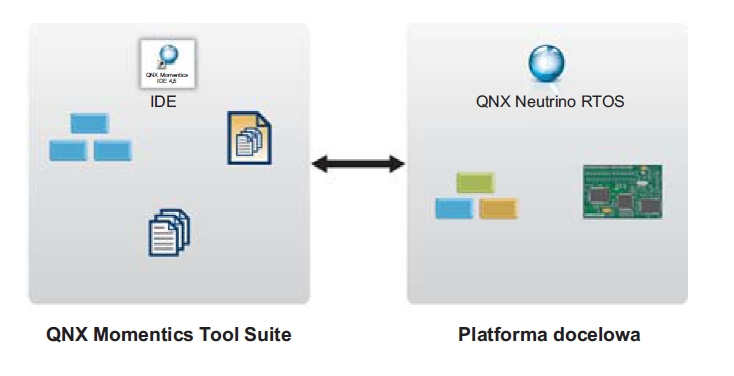
\includegraphics[width=0.35\textwidth]{img/qnxMomentics}
\caption{Platforma rozwoju oprogramowania}
\label{fig:qnxMomentics}
\end{figure}

Dzięki platformie programistycznej możemy tworzyć oprogramowanie w konfiguracji cross development (host-target). Na maszynie typu host (Windows) będziemy dysponować platformą programistyczną QNX Momentics, natomiast na maszynie docelowej typu target (QNX Neutrino na maszynie wirtualnej) będziemy uruchamiać nasze programy. Komunikacja pomiędzy komputerem host i target odbywa się przez sieć, a wspomaga go proces \lstinline[style=MyBashStyle]{qconn}.

\begin{figure}[!h]
\centering
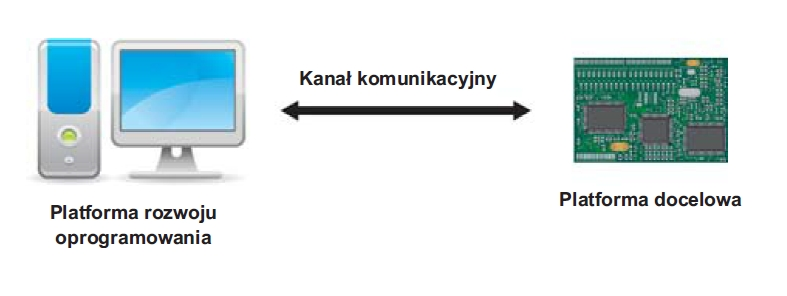
\includegraphics[width=0.5\textwidth]{img/konfiguracja}
\caption{Konfiguracja host-target}
\label{fig:konfiguracja}
\end{figure}

Niniejsze laboratorium będzie poswięcone kilka zagadnieniom:
\begin{myenumerate}
\item Podstawy obsługi QNX Momentics
\item Zarządzanie projektami C/C++
\item Edycja kodu źródłowego, kompilacja i~budowanie
\item Dostęp do platformy docelowej oraz uruchamianie aplikacji
\end{myenumerate}

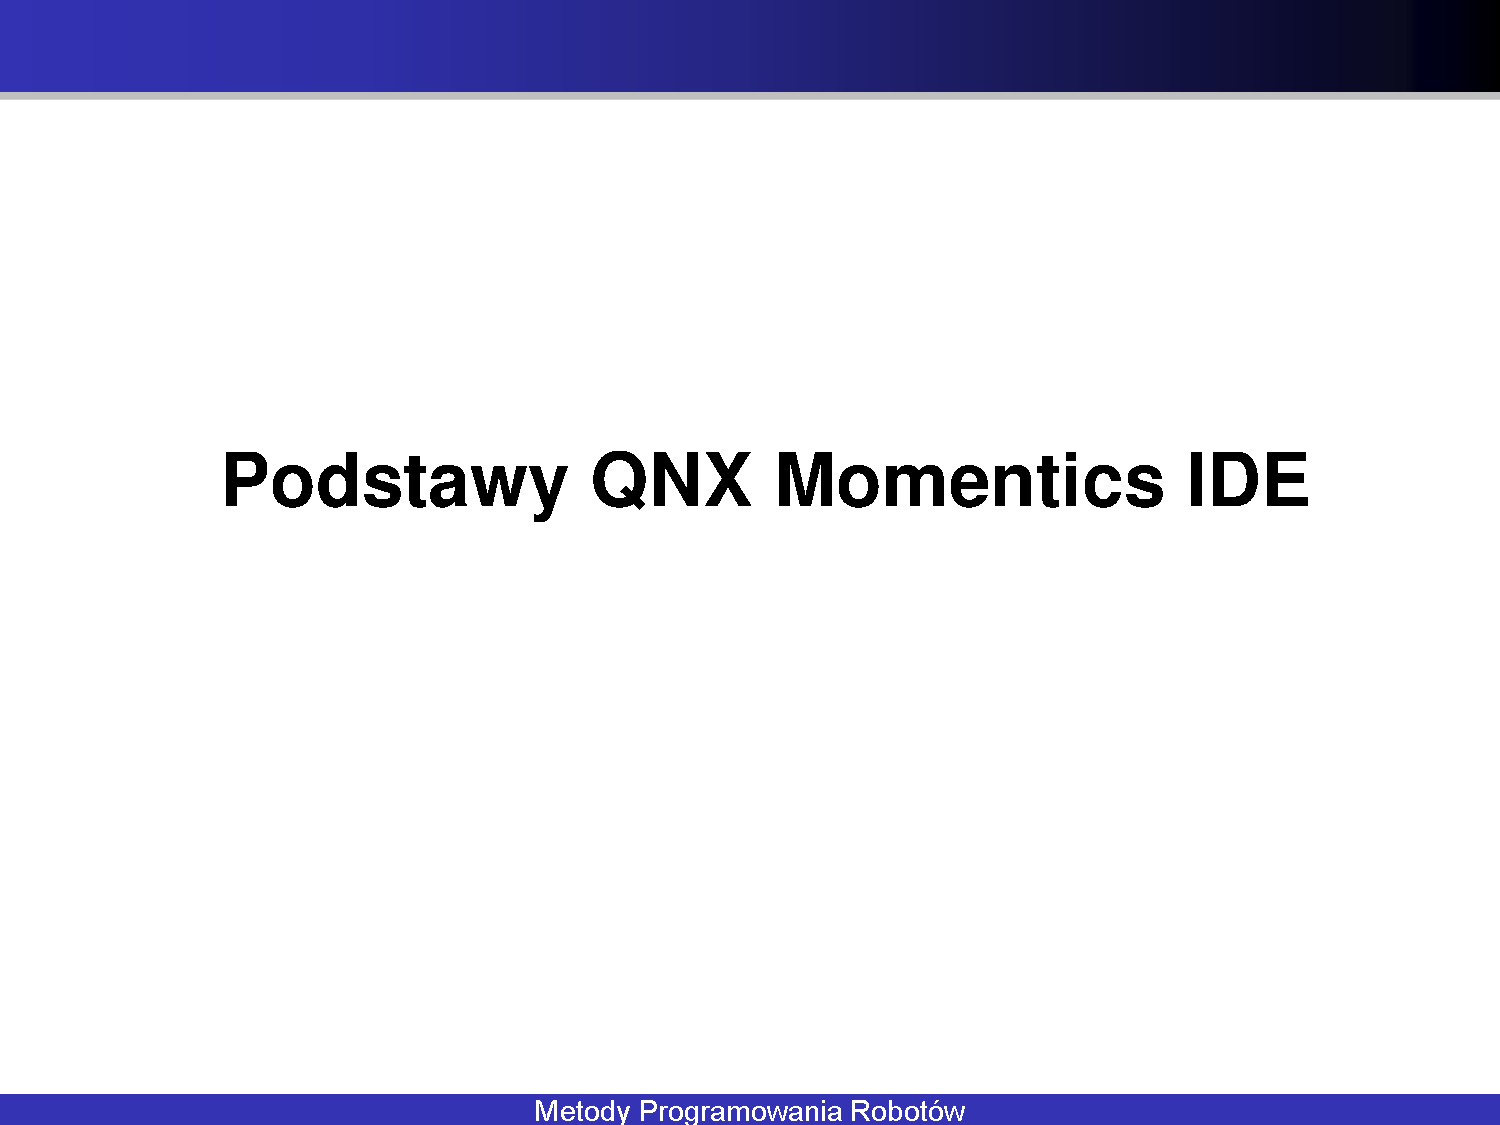
\includepdf[scale=0.75,pages={1-8},pagecommand={\thispagestyle{fancy}{\subsection{Podstawy obsługi QNX Momentics}}},nup=2x4]{img/qnx1.pdf}
\includepdf[scale=0.75,pages={9-},pagecommand={\thispagestyle{fancy}{}},nup=2x4]{img/qnx1.pdf}



\includepdf[scale=0.75,pages={1-8},pagecommand={\thispagestyle{fancy}{\subsection{Zarządzanie projektami C/C++}}},nup=2x4]{img/qnx2.pdf}

\includepdf[scale=0.75,pages={9-},pagecommand={\thispagestyle{fancy}{}},nup=2x4]{img/qnx2.pdf}



\includepdf[scale=0.75,pages={1-8},pagecommand={\thispagestyle{fancy}{\subsection{Edycja kodu, kompilacja i~budowanie}}},nup=2x4]{img/qnx3.pdf}

\includepdf[scale=0.75,pages={9-},pagecommand={\thispagestyle{fancy}{}},nup=2x4]{img/qnx3.pdf}


\includepdf[scale=0.75,pages={1-8},pagecommand={\thispagestyle{fancy}{\subsection{Dostęp do platformy docelowej oraz uruchamianie aplikacji}}},nup=2x4]{img/qnx4.pdf}

\includepdf[scale=0.75,pages={9-},pagecommand={\thispagestyle{fancy}{}},nup=2x4]{img/qnx4.pdf}

%\clearpage
%\phantomsection
%{\label{viRef}
%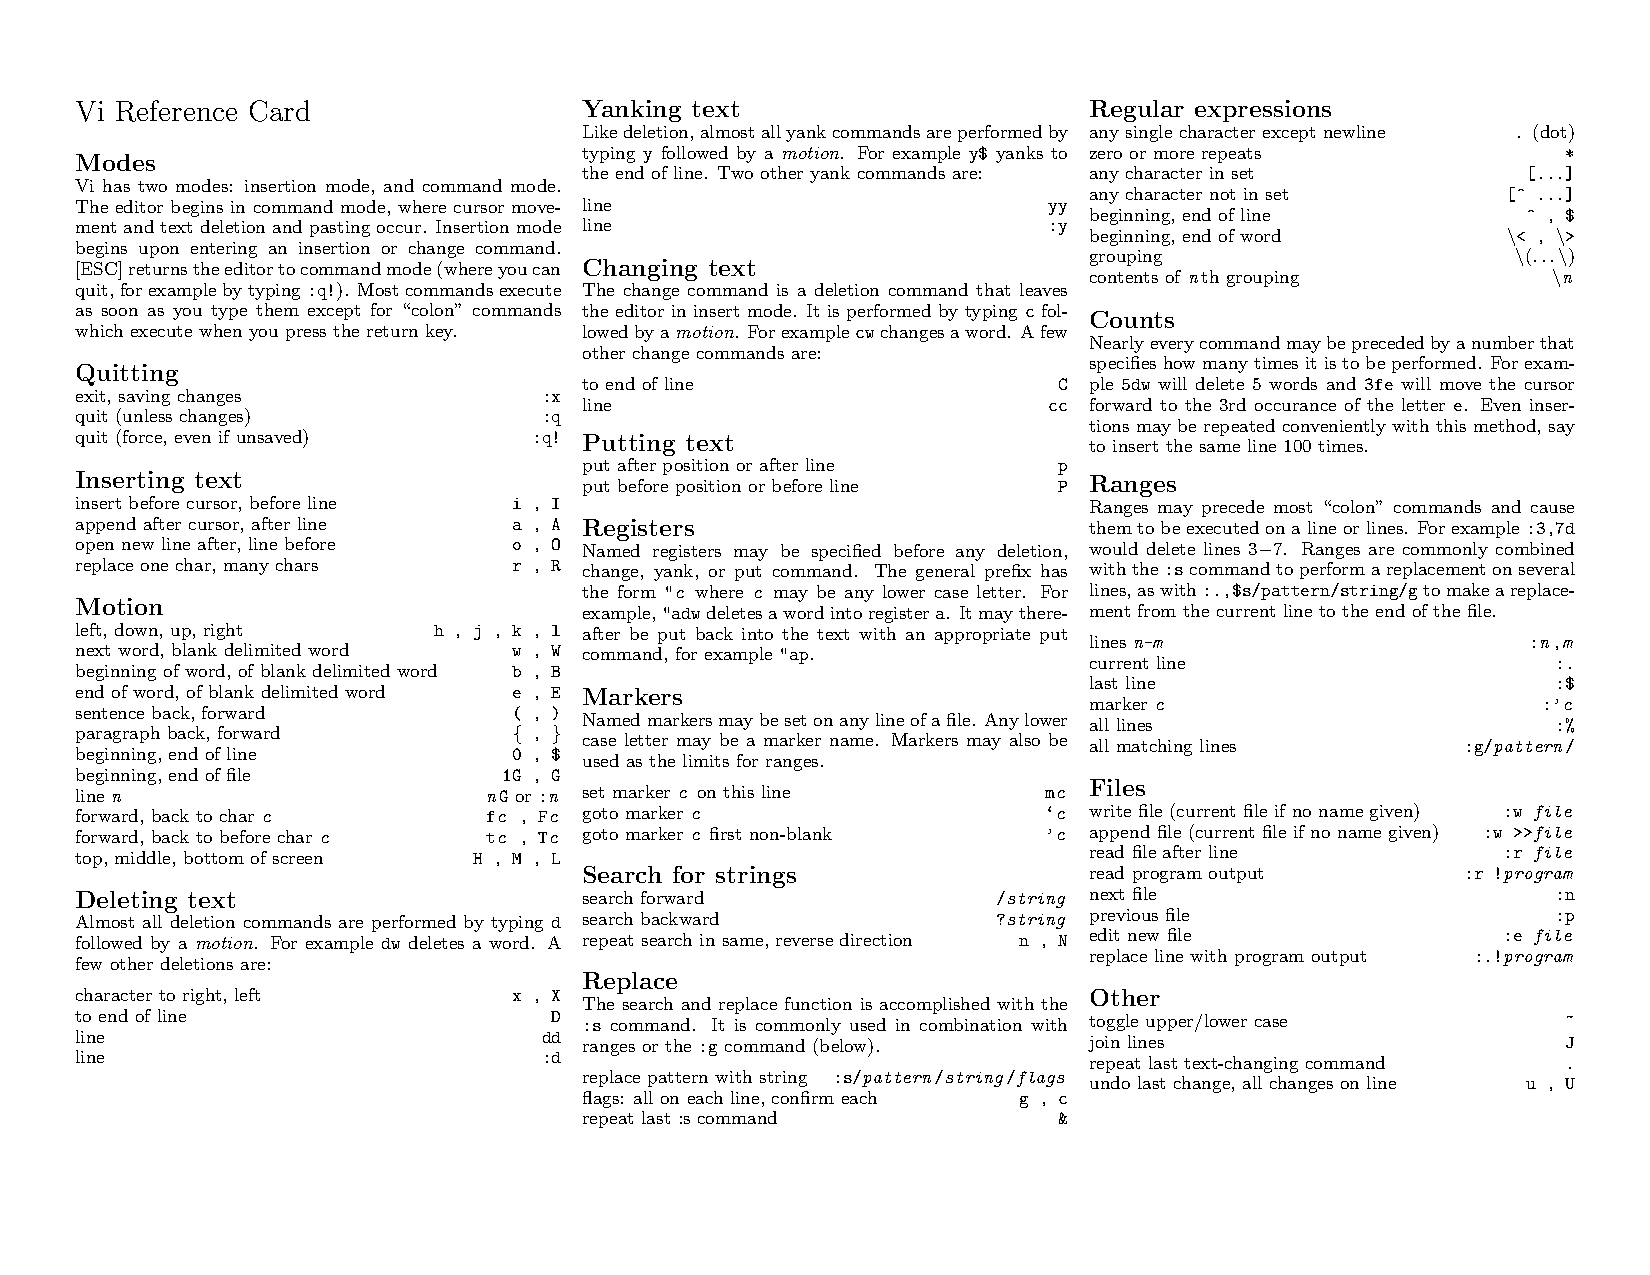
\includepdf[scale=0.95,pages={1},pagecommand={\thispagestyle{fancy}},pagecommand={\thispagestyle{fancy}{\label{subsec:vi}}},lastpage=1,angle=90]{img/viRef.pdf}
%}

%\subsection{Zarządzanie projektami C}
%
%\subsection{Edycja kodu źródłowego, kompilacja i~budowanie}
%
%\subsection{Dostęp do platformy docelowej oraz uruchamianie aplikacji}
%\subsection{Ćwiczenia}

\cleardoublepage

\section{Wprowadzenie do programowania w~języku C}

\subsection{Wstęp}
Treść laboratorium zawiera krótkie wprowadzenie do języka programowania C jako tego, który będzie wiodący w dalszych etapach zajęć. Wprowadzenie to pozwoli zacząć programować w języku C, tak szybko, jak to możliwe. Nie należy jednak traktować tej części laboratorium, jako substytutu kursów języka C, prezentowanych na innych wykładach i laboratoriach oraz w podręcznikach poświęconych językowi C. Pozostałe podrozdziały omawiają również podstawy użytkowania kompilatora oraz narzędzi make obecnych w~systemie QNX.

\subsection{Kompilowanie i~uruchamianie programów}

\subsubsection{Kompilator qcc}

Kody źródłowe, napisane w języku C muszą zostać wstępnie przetworzone (preprocessing), skompilowane (compiling) i skonsolidowane (linking), aby utworzyć plik wykonywalny. Używając linii poleceń, napisany program można skompilować w systemie QNX za pomocą następujących komend:


Dla języka C:

\begin{lstlisting}[style=MyBashStyle]
qcc [opcje] [operandy]
\end{lstlisting}

Dla języka C++:

\begin{lstlisting}[style=MyBashStyle]
QCC [opcje] [operandy]
\end{lstlisting}

Wybrane opcje kompilatora qcc zestawiono w~tabeli~, natomiast operandy stanowią pliki źródłowe (\lstinline[style=MyBashStyle]{*.c}) oraz pliki typu (\lstinline[style=MyBashStyle]{*.o}).

\begin{table}[h!]
\centering
\caption{Wybrane opcje kompilatora \lstinline[style=MyBashStyle]{qcc}}
\setlength{\arrayrulewidth}{1pt}
\setlength{\tabcolsep}{6pt}
\renewcommand{\arraystretch}{1.2}
\begin{tabular}{ |p{0.20\textwidth}|p{0.4\textwidth}|}
\hline \rowcolor{gray}
\textbf{Opcje} & \textbf{Opis} \\ \hline
\mbox{\lstinline[style=MyBashStyle]{-c}} & Tylko kompilacja \\ \hline
\mbox{\lstinline[style=MyBashStyle]{-E}} & Preprocessing na standardowe wyjście \\ \hline
\mbox{\lstinline[style=MyBashStyle]{-g}} & Kompilacja z debugowaniem \\ \hline
\mbox{\lstinline[style=MyBashStyle]{-I path [:path ...]}} & Ustawia ścieżkę przeszukiwania dla dyrektyw \mbox{\lstinline[style=MyBashStyle]{#include}}  \\ \hline
\mbox{\lstinline[style=MyBashStyle]{-L path [:path ...]}} & Ustawia ścieżkę przeszukiwania dla bibliotek  \\ \hline
\mbox{\lstinline[style=MyBashStyle]{-lplik}} & Dołącza bibliotekę o nazwie lib\underline{plik}.a lub lib\underline{plik}.so.  \\ \hline
\mbox{\lstinline[style=MyBashStyle]{-O1}} & Kompilowanie z optymalizacją \mbox{\lstinline[style=MyBashStyle]{O1}}.  \\ \hline
\mbox{\lstinline[style=MyBashStyle]{-O2}} & Kompilowanie z optymalizacją \mbox{\lstinline[style=MyBashStyle]{O2}}.  \\ \hline
\mbox{\lstinline[style=MyBashStyle]{-O3}} & Kompilowanie z optymalizacją \mbox{\lstinline[style=MyBashStyle]{O3}}.  \\ \hline
\mbox{\lstinline[style=MyBashStyle]{-o outfile}} & Ustala nazwę pliku wyjściowego (wykonywalnego). Domyślnie \mbox{\lstinline[style=MyBashStyle]{a.out}}.  \\ \hline
\mbox{\lstinline[style=MyBashStyle]{-Wall}} & Wyświetla wszystkie ostrzeżenia kompilatora.  \\ \hline
\mbox{\lstinline[style=MyBashStyle]{-pedantic}} & Wyświetla wszystkie ostrzeżenia kompilatora wymagane przez ANSI C.  \\ \hline
\end{tabular}
\label{tab:opcjeqcc}
\end{table}


\begin{example}[Konfiguracja środowiska pracy]
W~trakcie tego laboratorium będziemy głównie pracować w~linii poleceń. Zanim przejdziemy do właściwych przykładów, musimy skonfigurować środowisko pracy.

\begin{myenumerate}
\item  Ustawiamy zmienne środowiskowe w~systemie Windows. W tym celu należy:
\begin{myitemize}
\item Otworzyć linię poleceń w~systemie Windows, tj. nacisnąć przycisk \lstinline[style=MyBashStyle]{Start}, a~w~okienku \lstinline[style=MyBashStyle]{Wyszukaj programy i pliki} wpisać nazwę \lstinline[style=MyBashStyle]{cmd}.
\item W linii poleceń, uruchomić skrypt \lstinline[style=MyBashStyle]{C:\qnx660\qnx660-env.bat}.
\end{myitemize}

\item Na pulpicie tworzymy katalog o~nazwie \lstinline[style=MyBashStyle]{tmp}.
\item W~linii poleceń przechodzimy do katalogu \lstinline[style=MyBashStyle]{tmp} wpisując komendę \lstinline[style=MyBashStyle]{cd C:\Users\prog_N\Desktop\tmp}, gdzie \lstinline[style=MyBashStyle]{N} jest numerem komputera, do którego zalogowany jest użytkownik.
\item Uruchamiamy maszynę wirtualną z~systemem operacyjnym QNX oraz sprawdzamy IP maszyny za pomocą polecenia \lstinline[style=MyBashStyle]{ifconfig}.
\item Uruchamiamy środowisko do programowania aplikacji QNX Momentics oraz konfigurujemy dostęp do platformy docelowej w~kartach \lstinline[style=MyBashStyle]{Target Navigator} oraz \lstinline[style=MyBashStyle]{Target File System Navigator}.
\end{myenumerate}
\end{example}

\begin{example}[Pierwszy program...] \label{ex:pierwszy}

Otworzyć edytor tekstu \lstinline[style=MyBashStyle]{Notatnik}. Wpisać treść poniższego kodu i~zapisać plik pod nazwą \lstinline[style=MyBashStyle]{hello.c} w~katalogu \lstinline[style=MyBashStyle]{tmp} na \lstinline[style=MyBashStyle]{Pulpicie}.

\lstinputlisting[caption=Pierwszy program...,style=MyCStyle,label=src:kod3]{src/lab3/hello.c}

W~linii poleceń (Windows) skompilować program \lstinline[style=MyBashStyle]{hello.c} wydając polecenie:

\begin{lstlisting}[style=MyBashStyle]
> qcc -Wall hello.c
> ls
...
\end{lstlisting}

Proces tworzenia pliku wykonywalnego z~nadaniem nazw plików wyjściowych można podzielić na dwa etapy: kompilacja i~budowanie.

\begin{lstlisting}[style=MyBashStyle]
> qcc -Wall -c hello.c
> qcc hello.o -o hello
> ls
...
\end{lstlisting}

Kod źródłowy \lstinline[style=MyBashStyle]{hello.c} możemy jednocześnie skompilować i~zbudować z~nadaniem nazwy plikowi wyjściowemu.

\begin{lstlisting}[style=MyBashStyle]
> qcc -Wall hello.c -o hello2
> ls
...
\end{lstlisting}

Ostatnim etapem tego przykładu będzie uruchomienie programu \lstinline[style=MyBashStyle]{hello} na maszynie z~systemem operacyjnym QNX. Poprzez widok \lstinline[style=MyBashStyle]{Target File System Navigator} w środowisku QNX Momentics przekopiować program wykonywalny \lstinline[style=MyBashStyle]{hello} z~katalogu \lstinline[style=MyBashStyle]{tmp} do katalogu \lstinline[style=MyBashStyle]{/home} na maszynie wirtualnej. Uruchomić program poprzez polecenie:

\begin{lstlisting}[style=MyBashStyle]
# ./hello

Hello world !!!

#
\end{lstlisting}
\end{example}

\subsubsection{Sterowanie procesem budowania programów}

Kompilacja i uruchamianie projektu, składającego się z wielu plików źródłowych, w których zależności są złożone, może być uciążliwa. Istnieją programy narzędziowe, które ułatwiają zarządzanie złożonymi programami. Jednym z nich jest narzędzie \lstinline[style=MyBashStyle]{make}, które przetwarza specjalny plik \lstinline[style=MyBashStyle]{Makefile}.

W pliku \lstinline[style=MyBashStyle]{Makefile} występują tzw. reguły (ang. rules) mające następującą formę:

\begin{lstlisting}[style=MyBashStyle]
target: prerequisite [prerequisites]
<tab> commands
\end{lstlisting}

Cel (ang. target) - jest zazwyczaj plikiem, który chcemy utworzyć. Zależność (ang. prerequisite) - do utworzenia celu wymagane są zazwyczaj pliki źródłowe; nazywamy je zależnościami. Polecenia (ang. commands) - są krokami (np. wywołania kompilatora lub polecenia powłoki), które należy wykonać, aby utworzyć cel.

\begin{example}[Pierwszy plik Makefile]
W~Notatniku napisać skrypt \lstinline[style=MyBashStyle]{Makefile} do uruchomienia programu zapisanego w~\lstinline[style=MyBashStyle]{hello.c} oraz zapisać go w~katalogu \lstinline[style=MyBashStyle]{tmp}.

\begin{lstlisting}[style=MyBashStyle,caption=Pierwszy plik Makefile]
all: hello
hello: hello.o
	@echo "buduje..."
	qcc hello.o –o hello
hello.o: hello.c
	@echo "kompiluje..."
	qcc –Wall -c hello.c
clean:
	@echo "usuwam..."
	rm -f hello hello.o
\end{lstlisting}

Wpisać w~wiersz poleceń (Windows) następujące wywołania:

\begin{lstlisting}[style=MyBashStyle,caption=Pierwszy plik Makefile]
> make -n
> make all
> ls
...
> make clean
> ls
...
\end{lstlisting}

\end{example}


\begin{example}[Rozbudowany plik Makefile] \label{ex:rozbudowany}
W bardziej rozbudowanych projektach stosuje się różnego typu zmienne, które ułatwiają proces konstrukcji pliku \lstinline[style=MyBashStyle]{Makefile}. Należą do nich zmienne definiowane przez użytkownika, zmienne standardowe (predefiniowane), np. dotyczące nazw kompilatorów i~flag wywołań oraz zmienne automatyczne, których wartości są obliczane, gdy reguła jest wykonywana. Wybrane zmienne standardowe i~automatyczne przedstawiono w tabelach~\ref{tab:zmiennestandardowe} oraz \ref{tab:zmienneautomatyczne}.

\begin{table}[h!]
\centering
\caption{Zmienne standardowe}
\setlength{\arrayrulewidth}{1pt}
\setlength{\tabcolsep}{6pt}
\renewcommand{\arraystretch}{1.2}
\begin{tabular}{ |p{0.15\textwidth}|p{0.4\textwidth}|}
\hline \rowcolor{gray}
\textbf{Argumenty} & \textbf{Opis} \\ \hline
\mbox{\lstinline[style=MyBashStyle]{CC}} & Nazwa kompilatora języka C \\ \hline
\mbox{\lstinline[style=MyBashStyle]{CXX}} & Nazwa kompilatora języka C++ \\ \hline
\mbox{\lstinline[style=MyBashStyle]{CFLAGS}} & Opcje kompilatora języka C \\ \hline
\mbox{\lstinline[style=MyBashStyle]{CXXFLAGS}} & Opcje kompilatora języka C++  \\ \hline
\mbox{\lstinline[style=MyBashStyle]{LFLAGS}} & Opcje dla linkera  \\ \hline
\end{tabular}
\label{tab:zmiennestandardowe}
\end{table}


\begin{table}[h!]
\centering
\caption{Zmienne automatyczne}
\setlength{\arrayrulewidth}{1pt}
\setlength{\tabcolsep}{6pt}
\renewcommand{\arraystretch}{1.2}
\begin{tabular}{ |p{0.15\textwidth}|p{0.4\textwidth}|}
\hline \rowcolor{gray}
\textbf{Argumenty} & \textbf{Opis} \\ \hline
\mbox{\lstinline[style=MyBashStyle]{<}} & Nazwa pliku pierwszej zależności \\ \hline
\mbox{\lstinline[style=MyBashStyle]{@}} & Nazwa pliku docelowego \\ \hline
\mbox{\lstinline[style=MyBashStyle]{^}} & Lista wszystkich zależności \\ \hline
\end{tabular}
\label{tab:zmienneautomatyczne}
\end{table}

Zapisać w~Notatniku i uruchomić skrypt \lstinline[style=MyBashStyle]{Makefile} ze zmiennymi standardowymi i automatycznymi.


\begin{lstlisting}[style=MyBashStyle,caption=Rozbudowany plik Makefile]
CC=qcc
CFLAGS=-Wall
LFLAGS=-lm
SRC=hello.c
OBJS=hello.o
BINS=hello

all: $(BINS)
$(BINS): $(OBJS)
	@echo "buduje..."
	$(CC) $(LFLAGS) $^ -o $@
$(OBJS): $(SRC)
	@echo "kompiluje..."
	$(CC) $(CFLAGS) -c $< -o $@
clean:
	@echo "usuwam..."
	rm -f $(OBJS) $(BINS)
.PHONY: all clean
\end{lstlisting}
W przykładzie zastosowano zmienne definiowane przez użytkownika, zmienne standardowe oraz zmienne automatyczne. Dodatkowo użyto reguły \lstinline[style=MyBashStyle]{.PHONY}, służącej do poinstruowania narzędzia \lstinline[style=MyBashStyle]{make}, że reguły \lstinline[style=MyBashStyle]{all} oraz \lstinline[style=MyBashStyle]{clean} są regułami specjalnymi, a nie nazwami plików.
\end{example}


\begin{example}[Makefile w środowisku QNX Momentics]
Możemy wykorzystać plik \lstinline[style=MyBashStyle]{Makefile} utworzony w~przykładzie \ref{ex:rozbudowany} oraz kod źródłowy~\ref{src:kod3} zapisany w~przykładzie~\ref{ex:pierwszy} w~środowisku QNX Momentics. W~tym celu należy:

\begin{myenumerate}
\item W środowisku QNX Momentics utworzyć pusty projekt \lstinline[style=MyBashStyle]{C Project}, który należy nazwać jako \lstinline[style=MyBashStyle]{hello}.
\item Jako typ projektu wybrać \lstinline[style=MyBashStyle]{Empty project}, a~jako kompilator \lstinline[style=MyBashStyle]{QNX QCC}.
\item Zbudować projekt klikając prawym przyciskiem na projekt i~wciskając opcję \lstinline[style=MyBashStyle]{Build Project}.
\item Skonfigurować środowisko do uruchamiania programu i~uruchomić zbudowany program na maszynie QNX.
\item Usunąć pliki tymczasowe z~projektu klikając prawym przyciskiem na projekt i~wciskając opcję \lstinline[style=MyBashStyle]{Clean Project}.
\end{myenumerate}



\end{example}

\subsection{Podstawy języka C}

\subsubsection{Typy zmiennych}

Niektóre wbudowane typy zmiennych przedstawiono w~tabeli~\ref{tab:typyzmiennych}.

\begin{table}[h!]
\centering
\caption{Typy zmiennych}
\setlength{\arrayrulewidth}{1pt}
\setlength{\tabcolsep}{6pt}
\renewcommand{\arraystretch}{1.2}
\begin{tabular}{ |p{0.1\textwidth}|p{0.45\textwidth}|}
\hline \rowcolor{gray}
\textbf{Typ} & \textbf{Opis} \\ \hline
\mbox{\lstinline[style=MyBashStyle]{int}} & integer \\ \hline
\mbox{\lstinline[style=MyBashStyle]{short}} & short integer \\ \hline
\mbox{\lstinline[style=MyBashStyle]{long}} & long integer \\ \hline
\mbox{\lstinline[style=MyBashStyle]{float}} & single precision real (floating point) variable \\ \hline
\mbox{\lstinline[style=MyBashStyle]{double}} & double precision real (floating point) variable \\ \hline
\mbox{\lstinline[style=MyBashStyle]{char}} & character variable (single byte) \\ \hline
\end{tabular}
\label{tab:typyzmiennych}
\end{table}

\subsubsection{Pętle}

Większość programów zawiera pętle, umożliwiające powtarzanie określonych czynności. W języku C istnieje kilka różnych sposobów tworzenia pętli. Dwie najbardziej rozpowszechnione to pętla \lstinline[style=MyCStyle]{while} i~\lstinline[style=MyCStyle]{for}. Składnia poleceń podana jest poniżej.


\begin{lstlisting}[style=MyCStyle]
while (expression)
{
...block of statements to execute...
}
\end{lstlisting}

\begin{lstlisting}[style=MyCStyle]
for (expression_1; expression_2; expression_3)
{
...block of statements to execute...
}
\end{lstlisting}

Pętla \lstinline[style=MyCStyle]{while} jest kontynuowana dopóki wyrażenie logiczne jest prawdą, przy czym warunek ten jest sprawdzany po wejściu do pętli. Pętla \lstinline[style=MyCStyle]{for} jest równoważna następującej pętli \lstinline[style=MyCStyle]{while}.

\begin{lstlisting}[style=MyCStyle]
expression_1;
while (expression_2)
{
...block of statements...
expression_3;
}
\end{lstlisting}

Przykłady zastosowania pętli.

\begin{myitemize}
\item Pętla \lstinline[style=MyCStyle]{while}.
\end{myitemize}

\begin{lstlisting}[style=MyCStyle]
i = initial_i;

while (i < i_max)
{
...block of statements...
i = i + i_increment;
}
\end{lstlisting}

\begin{myitemize}
\item Pętla \lstinline[style=MyCStyle]{for}.
\end{myitemize}

\begin{lstlisting}[style=MyCStyle,caption=Pętla for - przykład]
for (i = initial_i; i <= i_max; i = i + i_increment)
{
...block of statements...
}
\end{lstlisting}


\subsubsection{Konstrukcje warunkowe}

\subsubsection{Operatory relacji}

\begin{table}[h!]
\centering
\caption{Operatory relacji}
\setlength{\arrayrulewidth}{1pt}
\setlength{\tabcolsep}{6pt}
\renewcommand{\arraystretch}{1.2}
\begin{tabular}{ |p{0.15\textwidth}|p{0.4\textwidth}|}
\hline \rowcolor{gray}
\textbf{Typ} & \textbf{Opis} \\ \hline
\mbox{\lstinline[style=MyBashStyle]{<}} & smaller than \\ \hline
\mbox{\lstinline[style=MyBashStyle]{<=}} & smaller than or equal to \\ \hline
\mbox{\lstinline[style=MyBashStyle]{==}} & equal to \\ \hline
\mbox{\lstinline[style=MyBashStyle]{!=}} & not equal to \\ \hline
\mbox{\lstinline[style=MyBashStyle]{>=}} & greater than or equal to \\ \hline
\mbox{\lstinline[style=MyBashStyle]{>}} & greater than \\ \hline
\end{tabular}
\label{tab:operatoryrelacji}
\end{table}



\subsubsection{Operatory logiczne}

\begin{table}[h!]
\centering
\caption{Operatory logiczne}
\setlength{\arrayrulewidth}{1pt}
\setlength{\tabcolsep}{6pt}
\renewcommand{\arraystretch}{1.2}
\begin{tabular}{ |p{0.15\textwidth}|p{0.4\textwidth}|}
\hline \rowcolor{gray}
\textbf{Typ} & \textbf{Opis} \\ \hline
\mbox{\lstinline[style=MyBashStyle]{&&}} & and \\ \hline
\mbox{\lstinline[style=MyBashStyle]{||}} & or \\ \hline
\mbox{\lstinline[style=MyBashStyle]{!}} & not \\ \hline
\end{tabular}
\label{tab:operatorylogiczne}
\end{table}

\subsubsection{Wskaźniki}

\begin{figure}[!h]
\centering
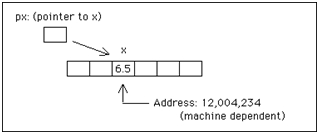
\includegraphics[width=0.5\textwidth]{img/pointer}
\caption{Idea wskaźnika}
\label{fig:wskaznik}
\end{figure}


\subsubsection{Tablice}

\begin{figure}[!h]
\centering
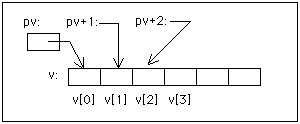
\includegraphics[width=0.5\textwidth]{img/tablica}
\caption{Tablica a~wskaźnika}
\label{fig:tablica}
\end{figure}

\subsubsection{Funkcje}

\subsubsection{Przekazywanie argumentów z wiersza poleceń}

\subsubsection{Operacje I/O (wejścia/wyjścia)}

\subsubsection{Operacje I/O na plikach}

\begin{table}[h!]
\centering
\caption{Operacje na plikach}
\setlength{\arrayrulewidth}{1pt}
\setlength{\tabcolsep}{6pt}
\renewcommand{\arraystretch}{1.2}
\begin{tabular}{ |p{0.15\textwidth}|p{0.4\textwidth}|}
\hline \rowcolor{gray}
\textbf{Typ} & \textbf{Opis} \\ \hline
\mbox{\lstinline[style=MyBashStyle]{r}} & czytanie z~pliku \\ \hline
\mbox{\lstinline[style=MyBashStyle]{w}} & pisanie do pliku \\ \hline
\mbox{\lstinline[style=MyBashStyle]{a}} & dodanie zawartości do pliku \\ \hline
\end{tabular}
\label{tab:operacjenaplikach}
\end{table}



\subsection{Ćwiczenia}


%\lstinline[style=MyBashStyle]{}
%\begin{lstlisting}[style=MyBashStyle,caption=Rozbudowany plik Makefile]
%\end{lstlisting}

\begin{myenumerate}
\item Zmodyfikować program obliczający tablicę funkcji \lstinline[style=MyBashStyle]{sinus}, tak, aby zawierał instrukcję sterującą \lstinline[style=MyBashStyle]{for}. Utworzyć funkcję \lstinline[style=MyBashStyle]{sinus} i przenieść jej kod do oddzielnego pliku źródłowego \lstinline[style=MyBashStyle]{sinus.c}. Dołączyć plik nagłówkowy \lstinline[style=MyBashStyle]{sinus.h} z~deklaracją funkcji. Napisać odpowiedni skrypt \lstinline[style=MyBashStyle]{Makefile}. Wyniki zapisać do pliku \lstinline[style=MyBashStyle]{sinus.dat}.
\item Napisz funkcję sprawdzającą ile par liczb całkowitych z przedziału \lstinline[style=MyBashStyle]{<a,b>} jest zawartych w~kole o~średnicy \lstinline[style=MyBashStyle]{8}. ($x^2+y^2\leq 8$). Wartości \lstinline[style=MyBashStyle]{a} i~\lstinline[style=MyBashStyle]{b} powinny być zadawane z klawiatury i przekazywane jako parametry funkcji.
\item Napisać bibliotekę operacji wektorowych, wykorzystując struktury. Zdefiniować wektor jako strukturę:

\begin{lstlisting}[style=MyCStyle]
struct Wektor
{
	double x, y, z;
};
\end{lstlisting}

Biblioteka operacji powinna pozwalać na dodawanie, odejmowanie, mnożenie przez liczbę wektora, liczenie iloczynów skalarnych i~wektorowych. Uzupełnić program  o odpowiednie funkcje testowe.
\item Uzupełnić poprzedni program o operacje transformacji wektorów z układu do układu. Napisać funkcje odpowiadające za elementarne obroty wokół osi \lstinline[style=MyBashStyle]{x}, \lstinline[style=MyBashStyle]{y}, \lstinline[style=MyBashStyle]{z}.
\end{myenumerate}




\cleardoublepage

\section{Procesy i zarządzanie procesami}

\subsection{Wstęp}

Przykłady procesów w życiu codziennym: proces fizyczny, chemiczny,
technologiczny, proces sądowy, administracyjny. Proces to przebieg powiązanych
ze sobą zmian. Większość procesów zachodzi w~określonym środowisku (np.
w~urzędzie), podlega pewnym ograniczeniom (np.  procedurom prawnym) i~wymaga
pewnych zasobów (np.  pieniędzy podatników). Pewne zdarzenia w~procesie
mogą występować sekwencyjnie, inne mogą nakładać się na siebie w~czasie. Jeśli
jesteśmy w~stanie wyodrębnić unikalny ciąg występujących po sobie zdarzeń
i~stwierdzić, że są ze sobą jakoś powiązane, to taką sekwencję często określa
się mianem wątku. Proces, podobnie jak fabuła powieści, może obejmować wiele
wątków biegnących równocześnie.

W~informatyce proces jest dynamicznym obiektem utworzonym przez system
operacyjny w~celu wykonania pewnego programu. Procesowi przydzielane są zasoby
takie jak czas procesora, obszar pamięci operacyjnej, pliki, urządzenia
peryferyjne. W~pamięci komputera zwykle znajduje się wiele procesów, które są
na różnych etapach wykonania i~współzawodniczą o~zasoby. W~obrębie jednego
procesu występuje jeden lub więcej wątków (w uproszczeniu wątek obrazuje ciąg
wykonywanych po sobie instrukcji procesora), wątki mogą być wykonywane
równolegle (tj. wątek A biegnie równolegle z~wątkiem B).

Często proces jest utożsamiany z~programem uruchomionym w~systemie operacyjnym.
Rzeczywiste aplikacje mogą się jednak składać z~wielu procesów, które
komunikują się ze sobą za pomocą mechanizmów komunikacji międzyprocesowej
(inter-process communication, IPC). Zagadnieniom komunikacji IPC poświęcono
odrębne rozdziały tej instrukcji.

Obiekt-proces (tak jak większość obiektów w~informatyce) posiada pewne atrybuty,
oraz podlega regułom określającym jego czas życia. W~niniejszym laboratorium
omówimy następujące zagadnienia:
\begin{myitemize}
  \item wyświetlanie i~modyfikowanie atrybutów procesów (atrybuty),
  \item tworzenie i usuwanie procesów (czas życia).
\end{myitemize}

\subsection{Wyświetlanie i modyfikowanie atrybutów procesów}

Atrybuty to informacje przechowywane przez obiekt-proces na rzecz systemu
operacyjnego. Pozwalają systemowi i~użytkownikowi identyfikować procesy oraz
np. określać jakie zasoby są aktualnie przydzielone poszczególnym procesom.

Każdy proces w systemie QNX ma przypisany unikalny identyfikator PID (process
ID), który jest liczbą całkowitą. Każdy proces (oprócz procesu ,,głównego''
\texttt{procnto}) ma również swój proces macierzysty. Identyfikator PPID
(parent process ID) jest identyfikatorem PID procesu macierzystego. Proces
\texttt{procnto} ma identyfikator PID=1 i~nie ma identyfikatora PPID. Wybrane
atrybuty i~funkcje systemowe umożliwiające dostęp do nich przedstawiono
w~tabeli \ref{tab:HE6LE}.

%%%%%%%%%%%%%%%%%%%%%%%%%%%%%%%%%%%%%%%%%%%%%%%%%%%%%%%%%%%%%%%%%%%%%%%%%%%%%
\begin{table}[h!]
  \centering
  \caption{Niektóre atrybuty procesów oraz funkcje biblioteki systemowej
           umożliwiające dostęp do nich}
  \label{tab:HE6LE}
  \begin{tabular}{|c|c|c|}
    \hline
    \textbf{Atrybuty procesu} & \textbf{Wyświetlanie} & \textbf{Modyfikacja} \\ \hline
    Identyfikator PID                   & \texttt{getpid()}           & -- \\ \hline
    Identyfikator PPID                  & \texttt{getppid()}          & -- \\ \hline
    Priorytet i~strategia szeregowania  & \texttt{sched\_getparam()}  & \texttt{sched\_setparam()} \\ \hline
  \end{tabular}
\end{table}
%%%%%%%%%%%%%%%%%%%%%%%%%%%%%%%%%%%%%%%%%%%%%%%%%%%%%%%%%%%%%%%%%%%%%%%%%%%%%

Na ogół mamy do czynienia z sytuacją, kiedy procesów gotowych do wykonania jest
więcej niż umożliwiają to dostępne w~danej chwili zasoby. Procedura szeregująca
(scheduler) rozstrzyga, któremu z procesów (wątków) zostanie w~danej chwili
przydzielony czas procesora. Jednym z~istotnych parametrów rzutujących na
kolejność przydzielania czasu procesora jest priorytet -- każdy z procesów (i
wątków -- patrz następne laboratoria) ma przyporządkowany priorytet (process
priority).  Jest on miarą pilności wykonania danego procesu względem innych.
W systemie QNX Neutrino 6 priorytet jest liczbą z zakresu od 0 (najniższy) do
255 (najwyższy). System nakłada ograniczenia na dopuszczalne zakresy
priorytetów dla programów uruchamianych przez poszczególnych użytkowników
(tabela \ref{tab:2N6W7}):

%%%%%%%%%%%%%%%%%%%%%%%%%%%%%%%%%%%%%%%%%%%%%%%%%%%%%%%%%%%%%%%%%%%%%%%%%%%%%
\begin{table}[h!]
  \centering
  \caption{Priorytety w~QNX Neutrino 6}
  \label{tab:2N6W7}
  \begin{tabular}{|c|c|c|}
    \hline
    \textbf{Priorytet} & \textbf{Użytkownik} \\ \hline
    0 & Proces jałowy \\ \hline
    1 -- 63 & Wątki zwykłego użytkownika \\ \hline
    1 -- 255 & Wątki użytkownika \texttt{root} \\ \hline
  \end{tabular}
\end{table}
%%%%%%%%%%%%%%%%%%%%%%%%%%%%%%%%%%%%%%%%%%%%%%%%%%%%%%%%%%%%%%%%%%%%%%%%%%%%%

W systemie QNX są dostępne trzy strategie szeregowania:
\begin{myitemize}
  \item szeregowanie FIFO (FIFO scheduling),
  \item szeregowanie karuzelowe (round robin scheduling),
  \item szeregowanie sporadyczne (sporadic scheduling).
\end{myitemize}
Są one omówione szczegółowo w dokumentacji QNX~\cite{qnx}. W tabeli
\ref{tab:A9C2X} przedstawiono ich symbole, wykorzystywane w~wywołaniach
systemowych.


%%%%%%%%%%%%%%%%%%%%%%%%%%%%%%%%%%%%%%%%%%%%%%%%%%%%%%%%%%%%%%%%%%%%%%%%%%%%%
\begin{table}[h!]
  \centering
  \caption{Strategie szeregowania w~QNX Neutrino 6}
  \label{tab:A9C2X}
  \begin{tabular}{|c|c|c|}
    \hline
    \textbf{Symbol}           & \textbf{Opis} \\ \hline
    \texttt{SCHED\_FIFO}      & Szeregowanie FIFO \\ \hline
    \texttt{SCHED\_RR}        & Szeregowanie karuzelowe \\ \hline
    \texttt{SCHED\_SPORADIC}  & Szeregowanie sporadyczne \\ \hline
  \end{tabular}
\end{table}
%%%%%%%%%%%%%%%%%%%%%%%%%%%%%%%%%%%%%%%%%%%%%%%%%%%%%%%%%%%%%%%%%%%%%%%%%%%%%

%%%%%%%%%%%%%%%%%%%%%%%%%%%%%%%%%%%%%%%%%%%%%%%%%%%%%%%%%%%%%%%%%%%%%%%%%%%%%
\begin{example}{[Lista procesów]}
  \label{ex:TYRDA}
  W terminalu wykonać polecenie \texttt{ps -l}. Sprawdzić w {\color{red}dokumentacji},
  co oznaczają poszczególne kolumny wyświetlonego raportu.
\end{example}
%%%%%%%%%%%%%%%%%%%%%%%%%%%%%%%%%%%%%%%%%%%%%%%%%%%%%%%%%%%%%%%%%%%%%%%%%%%%%

%%%%%%%%%%%%%%%%%%%%%%%%%%%%%%%%%%%%%%%%%%%%%%%%%%%%%%%%%%%%%%%%%%%%%%%%%%%%%
\begin{example}{[Wyświetlanie i modyfikacja wybranych atrybutów procesu]}
  \label{ex:TEPBG}
  \lstinputlisting[style=MyCStyle,label=src:4JKQ7]{src/lab4/attributes1.c}
\end{example}
%%%%%%%%%%%%%%%%%%%%%%%%%%%%%%%%%%%%%%%%%%%%%%%%%%%%%%%%%%%%%%%%%%%%%%%%%%%%%


\subsection{Tworzenie procesów}

W systemie QNX Neutrino, modułem odpowiedzialnym za dynamiczne tworzenie,
usuwanie oraz zarządzanie procesami jest zawarty w mikrojądrze (procnto)
manager procesów. W systemie QNX istnieją różne metody tworzenia procesów.
Część z nich pochodzi wprost od systemów UNIX-owych, opartych o standard POSIX,
inne funkcje do tworzenia procesów są charakterystyczne tylko dla systemu QNX.
Podstawowe funkcje do tworzenia procesów przedstawiono w tabeli
\ref{tab:IMJR3}. W ramach laboratorium omówimy cztery funkcje, służące
tworzeniu procesów, tj. \texttt{system()}, \texttt{fork()}, \texttt{exec()},
\texttt{spawn()}.

%%%%%%%%%%%%%%%%%%%%%%%%%%%%%%%%%%%%%%%%%%%%%%%%%%%%%%%%%%%%%%%%%%%%%%%%%%%%%
\begin{table}[h!]
  \centering
  \caption{Metody tworzenia procesów w systemie QNX}
  \label{tab:IMJR3}
  \begin{tabular}{|l|p{0.75\textwidth}|}
    \hline
    \textbf{Funkcja}    & \textbf{Opis}  \\ \hline
    \texttt{system()}   & Wywołanie programów, poleceń systemowych, bądź skryptów \\ \hline
    \texttt{fork()}     & Utworzenie kopii procesu bieżącego \\ \hline
    \texttt{exec()}     & Zastąpienie bieżącego procesu nowym procesem -- rodzina funkcji \\ \hline
    \texttt{spawn()}    & Utworzenie procesu potomnego -- rodzina funkcji \\ \hline
    \texttt{vfork()}    & Utworzenie procesu potomnego i zablokowanie procesu macierzystego \\ \hline
    \texttt{forkpty()}  & Utworzenie procesu potomnego w oknie pseudoterminala \\ \hline
    \texttt{popen()}    & Uruchomienie programu jako procesu potomnego z
                          jednoczesnym utworzeniem łącza pomiędzy procesem
                          bieżącym, a potomnym \\ \hline
  \end{tabular}
\end{table}
%%%%%%%%%%%%%%%%%%%%%%%%%%%%%%%%%%%%%%%%%%%%%%%%%%%%%%%%%%%%%%%%%%%%%%%%%%%%%

Jednym z~najprostszych sposobów uruchomienia innego procesu z~poziomu programu
w~języku C jest użycie funkcji \texttt{system()} (przykład \ref{ex:V86MA}).
Poleceniem tym można uruchomić program w~sposób podobny, jak to się czyni
wprost z~powłoki. Funkcja zwraca status zakończenia uruchomionego programu.

%%%%%%%%%%%%%%%%%%%%%%%%%%%%%%%%%%%%%%%%%%%%%%%%%%%%%%%%%%%%%%%%%%%%%%%%%%%%%
\begin{example}{[Wywołanie programu za pomocą polecenia system()]}
  \label{ex:V86MA}
  \lstinputlisting[style=MyCStyle,label=src:P1A10]{src/lab4/system1.c}
\end{example}
%%%%%%%%%%%%%%%%%%%%%%%%%%%%%%%%%%%%%%%%%%%%%%%%%%%%%%%%%%%%%%%%%%%%%%%%%%%%%

Funkcja \texttt{fork()} tworzy kopię procesu i~uruchamia ją jako proces
potomny. Utworzony proces potomny wykonuje się współbieżnie z procesem
tworzącym, posiada własny nr PID, a jego PPID wskazuje na proces tworzący.
Funkcja \texttt{fork()} tworzy deskryptor nowego procesu oraz kopię segmentu
kodu, danych i stosu. Modyfikacje zmiennych w procesie macierzystym nie są
widoczne w procesie potomnym i odwrotnie. Jeżeli operacja utworzenia procesu
potomnego zakończy się powodzeniem, to funkcja w procesie macierzystym zwraca
identyfikator (PID) procesu potomnego (wartość większa od 1), a w procesie
potomnym wartość 0. Jeżeli próba utworzenia procesu się nie powiedzie, to
funkcja \texttt{fork()} zwraca w procesie macierzystym wartość -1. Działanie
funkcji przedstawiono na rysunku, a jej użycie w przykładzie~\ref{ex:HP9M8}.

%%%%%%%%%%%%%%%%%%%%%%%%%%%%%%%%%%%%%%%%%%%%%%%%%%%%%%%%%%%%%%%%%%%%%%%%%%%%%
\begin{figure}
  \centering
  \begin{tikzpicture}
    \node[TBox6emCentered] (parent)   at (0.00,3.50)  {Proces macierzysty};
    \node                  (fork)     at (0.00,1.75)  {\texttt{fork()}};
    \node                  (x)        at (4.50,1.75)  {};
    \node[TBox6emCentered] (parent2)  at (0.00,0.00)  {Proces macierzysty};
    \node[TBox6emCentered] (child)    at (4.50,0.00)  {Proces potomny};

    \draw[->] (parent.south)  to                                                (fork.north);
    \draw[->] (fork.south)    to node[anchor=center,left]{Zwraca PID potomka}   (parent2.north);
    \draw[->] (fork.east)     to                                                (x.center)
                              to node[anchor=center, right]{Zwraca zero}        (child.north);
  \end{tikzpicture}
  \caption{Idea działania funkcji \texttt{fork()}}
  \label{fig:S278F}
\end{figure}
%%%%%%%%%%%%%%%%%%%%%%%%%%%%%%%%%%%%%%%%%%%%%%%%%%%%%%%%%%%%%%%%%%%%%%%%%%%%%

%%%%%%%%%%%%%%%%%%%%%%%%%%%%%%%%%%%%%%%%%%%%%%%%%%%%%%%%%%%%%%%%%%%%%%%%%%%%%
\begin{example}{[Wywołanie funkcji fork()]}
  \label{ex:HP9M8}
  \lstinputlisting[style=MyCStyle,label=src:Z5EXB]{src/lab4/fork1.c}

  Sprawdzić działanie programu, gdy zmienna CHILD = 8, a zmienna PARENT = 4.
\end{example}
%%%%%%%%%%%%%%%%%%%%%%%%%%%%%%%%%%%%%%%%%%%%%%%%%%%%%%%%%%%%%%%%%%%%%%%%%%%%%

\subsection{Obsługa zakończenia procesów}

Poprawne zakończenie procesów jest zagadnieniem, na które należy zwrócić
szczególną uwagę przy rozwoju wiarygodnego oprogramowania w systemie QNX.
Powodem tego jest fakt, że procesy na ogół współdziałają ze sobą, mogą być np.
procesami macierzystymi, bądź oczekiwać na określone zdarzenia, wygenerowane
przez inne procesy. W związku z tym, przed zakończeniem procesu należy zwolnić
zajęte przez ten proces zasoby, zakończyć z innymi procesami scenariusze
komunikacyjne i synchronizacyjne oraz zaczekać na zakończenie procesów
potomnych.

Zakończenie procesu następuje w następujących przypadkach:
\begin{myitemize}
  \item poprzez wywołanie funkcji exit(),
  \item funkcja main() wywołuje instrukcję return lub zakończyło się działanie
        ostatniej instrukcji kodu,
  \item proces zostanie zakończony przez system operacyjny lub inny proces.
\end{myitemize}

Normalne zakończenie procesu może być zainicjowane przez programistę, poprzez
wywołanie funkcji \texttt{exit()}

%%%%%%%%%%%%%%%%%%%%%%%%%%%%%%%%%%%%%%%%%%%%%%%%%%%%%%%%%%%%%%%%%%%%%%%%%%%%%
\begin{lstlisting}[style=MyCStyle]
 #include <stdlib.h>
 void exit( int status );
\end{lstlisting}
%%%%%%%%%%%%%%%%%%%%%%%%%%%%%%%%%%%%%%%%%%%%%%%%%%%%%%%%%%%%%%%%%%%%%%%%%%%%%

Funkcja ta powoduje zakończenie procesu bieżącego oraz zwrócenie statusu
zakończonego procesu.  Status jest dostępny dla procesu macierzystego. Na ogół
wartość statusu jest ustawiana na \texttt{EXIT\_SUCCESS}, gdy proces zakończył
się poprawnie, bądź na wartość \texttt{EXIT\_FAILURE}, bądź innych kod, gdy
wystąpił błąd.

W przypadku, gdy proces macierzysty uruchamia procesy potomne, należy unikać
sytuacji, gdy proces macierzysty kończy się wcześniej, niż jego procesy potomne
(osierocenie procesów). Proces macierzysty powinien zaczekać na zakończenie
swoich procesów potomnych. Do synchronizacji zakończenia procesów używa się
funkcji:


%%%%%%%%%%%%%%%%%%%%%%%%%%%%%%%%%%%%%%%%%%%%%%%%%%%%%%%%%%%%%%%%%%%%%%%%%%%%%
\begin{lstlisting}[style=MyCStyle]
  #include <sys/types.h>
  #include <sys/wait.h>
  pid_t wait( int * status );
\end{lstlisting}
%%%%%%%%%%%%%%%%%%%%%%%%%%%%%%%%%%%%%%%%%%%%%%%%%%%%%%%%%%%%%%%%%%%%%%%%%%%%%

Zmienna \texttt{status} jest statusem zakończenia procesu potomnego. Funkcja
zwraca PID zakończonego procesu, bądź -1, w przypadku gdy brak procesów
potomnych. \texttt{wait()} blokuje proces wywołujący, do momentu, gdy któryś z procesów
potomnych zakończył się poprawnie (np. wywołał funkcję \texttt{exit()}), bądź
wystąpił błąd.

%%%%%%%%%%%%%%%%%%%%%%%%%%%%%%%%%%%%%%%%%%%%%%%%%%%%%%%%%%%%%%%%%%%%%%%%%%%%%
\begin{figure}
  \centering
  \begin{tikzpicture}
    \node[TBox6emCentered]  (parent)  at (0.00, 3.50) {Proces macierzysty};
    \node                   (fork)    at (0.00, 2.00) {\texttt{fork()}};
    \node                   (wait)    at (0.00, 0.75) {\texttt{wait()}};
    \node[TBox6emCentered]  (child)   at (4.50, 2.00) {Proces potomny};
    \node[circle,draw=black](o)       at (0.00,-0.25) {};
    \node                   (exit)    at (4.50,-0.25) {\texttt{exit()}};
    \node                   (end1)    at (0.00,-1.00) {};
    \node[circle,fill=black](end2)    at (4.50,-1.00) {};
    \node[right of = end2]  (end2t)   {Koniec};

    \draw[->] (parent.south)  to (fork.north);
    \draw[->] (fork.east)     to (child.west);
    \draw[->] (fork.south)    to (wait.north);
    \draw[->] (wait.south)    to node[anchor=center,left]{Oczekiwanie} (o.north);
    \draw[->] (child.south)   to (exit.north);
    \draw[->,dotted] (exit.west)     to (o.east);
    \draw[->] (o.south)       to node[anchor=center,left]{Dalszy bieg} (end1.south);
    \draw[->] (exit.south)    to (end2);
  \end{tikzpicture}
  \caption{Schemat poprawnego zakończenia procesu}
  \label{fig:Z6B8G}
\end{figure}
%%%%%%%%%%%%%%%%%%%%%%%%%%%%%%%%%%%%%%%%%%%%%%%%%%%%%%%%%%%%%%%%%%%%%%%%%%%%%

Ilustrację omawianych zagadnień stanowi niniejszy przykład.

%%%%%%%%%%%%%%%%%%%%%%%%%%%%%%%%%%%%%%%%%%%%%%%%%%%%%%%%%%%%%%%%%%%%%%%%%%%%%
\begin{example}{[Wywołanie funkcji fork() wraz z obsługą zakończenia procesów]}
  \label{ex:11SSB}
  \lstinputlisting[style=MyCStyle,label=src:92W6D]{src/lab4/process1.c}
\end{example}
%%%%%%%%%%%%%%%%%%%%%%%%%%%%%%%%%%%%%%%%%%%%%%%%%%%%%%%%%%%%%%%%%%%%%%%%%%%%%


Zastosowanie funkcji \texttt{wait()} zapewnia, że proces macierzysty nie zakończy się
przed procesem potomnym. W przypadku, gdy proces potomny zakończy się przed
wywołaniem przez macierzysty funkcji \texttt{wait()}, proces potomny zwalnia
wszystkie zasoby, z wyjątkiem deskryptora procesu, czyli miejsca w pamięci
operacyjnej, gdzie przechowywane są wszystkie informacje potrzebne do
zarządzania procesem. Status zakończenia procesu potomnego jest przekazywany do
procesu macierzystego w deskryptorze procesu potomnego. Taki stan procesu
potomnego nazywa się stanem ,,zombie''.

Inną funkcją, pozwalającą na oczekiwanie na zakończenie konkretnego procesu
potomnego jest funkcja \texttt{waitpid()}.

%%%%%%%%%%%%%%%%%%%%%%%%%%%%%%%%%%%%%%%%%%%%%%%%%%%%%%%%%%%%%%%%%%%%%%%%%%%%%
\begin{lstlisting}[style=MyCStyle]
#include <sys/types.h>
#include <sys/wait.h>

pid_t waitpid( pid_t pid, int *status, int options );
\end{lstlisting}
%%%%%%%%%%%%%%%%%%%%%%%%%%%%%%%%%%%%%%%%%%%%%%%%%%%%%%%%%%%%%%%%%%%%%%%%%%%%%

Funkcja zwraca PID zakończonego procesu, bądź -1, w przypadku, gdy brak jest
procesów potomnych. Funkcja zwraca również status zakończonego procesu poprzez
argument \texttt{status}. Jedną z użytecznych opcji funkcji jest flaga
\texttt{WNOHANG}, która powoduje, że proces macierzysty, w przypadku braku
potomnych, natychmiast wraca z funkcji i kontynuuje swoje działanie i w tym
przypadku możemy użyć takiej kombinacji do cyklicznego sprawdzania, czy proces
potomny się zakończył.


\subsection{Zastąpienie procesu bieżącego innymi procesami}

Funkcje z rodziny exec() zastępują bieżący proces, nowym procesem, na podstawie
pliku wykonywalnego, którego nazwa jest parametrem funkcji. W odróżnieniu od
funkcji \texttt{fork()},  w przypadku użytkowania funkcji z rodziny
\texttt{exec()}, kody procesów macierzystych i potomnych mogą być umieszczone w
oddzielnych plikach źródłowych. Taka konfiguracja zapewnia łatwiejsze
uruchamianie i testowanie programów. W systemie QNX zdefiniowano następującą
rodzinę funkcji: \texttt{execl()}, \texttt{execle()}, \texttt{execlp()},
\texttt{execlpe()}, \texttt{execv()}, \texttt{execve()}, \texttt{execvp()},
\texttt{execvpe()}. Działanie tych funkcji jest podobne, natomiast różnią się
listą parametrów formalnych. W trakcie laboratorium będziemy używać
najprostszych funkcji \texttt{execl()} oraz \texttt{execv()}, których sygnatury
wyglądają następująco:

%%%%%%%%%%%%%%%%%%%%%%%%%%%%%%%%%%%%%%%%%%%%%%%%%%%%%%%%%%%%%%%%%%%%%%%%%%%%%
\begin{lstlisting}[style=MyCStyle]
#include <process.h>

int execl(  const char * path,
            const char * arg0,
            const char * arg1,
            ...
            const char * argn,
            NULL );
int execv( const char * path,
           char * const argv[] );
\end{lstlisting}
%%%%%%%%%%%%%%%%%%%%%%%%%%%%%%%%%%%%%%%%%%%%%%%%%%%%%%%%%%%%%%%%%%%%%%%%%%%%%

gdzie \texttt{path} jest ścieżką do pliku wykonywalnego, a argumenty
\texttt{arg[0]} do \texttt{arg[n]} -- nazwą i argumentami programu. Na ostatnim
miejscu podaje się wartość \texttt{NULL}, na oznaczenie zakończenia listy
parametrów wywoływanego programu.

Funkcja \texttt{execv()} pobiera tylko dwa argumenty i daje możliwość
elastycznego budowania listy parametrów. Drugi z argumentów jest tablicą
napisów, która musi być zakończona pustym wskaźnikiem \texttt{((char *)0)}.
Wartość pola \texttt{argv[0]} musi wskazywać na nazwę procesu, który chcemy
uruchomić.

%%%%%%%%%%%%%%%%%%%%%%%%%%%%%%%%%%%%%%%%%%%%%%%%%%%%%%%%%%%%%%%%%%%%%%%%%%%%%
\begin{example}{[Wywołanie funkcji execl()]}
  \label{ex:WHF3V}
  \lstinputlisting[style=MyCStyle,label=src:5Y0UB]{src/lab4/execv1.c}
\end{example}
%%%%%%%%%%%%%%%%%%%%%%%%%%%%%%%%%%%%%%%%%%%%%%%%%%%%%%%%%%%%%%%%%%%%%%%%%%%%%

\subsection{Tworzenie procesów funkcją spawn()}

Posługiwanie się funkcjami \texttt{fork()} i \texttt{exec()} do tworzenia
procesów współbieżnych bywa niewygodne. System operacyjny QNX udostępnia
rodzinę \texttt{spawn()}, która służy do tworzenia procesów potomnych na
podstawie pliku wykonywalnego, którego nazwa jest jednym z argumentów funkcji.
Do tej grupy zaliczamy następujące funkcje: \texttt{spawn()},
\texttt{spawnl()}, \texttt{spawnv()}, \texttt{spawnle()}, \texttt{spawnlp()},
\texttt{spawnlpe()}, \texttt{spawnve()}, \texttt{spawnvp()},
\texttt{spawnvpe()}. Ponownie omówimy tylko dwie wybrane funkcje
\texttt{spawnl()} i~\texttt{spawnv()}, których deklaracje wyglądają
następująco:

%%%%%%%%%%%%%%%%%%%%%%%%%%%%%%%%%%%%%%%%%%%%%%%%%%%%%%%%%%%%%%%%%%%%%%%%%%%%%
\begin{lstlisting}[style=MyCStyle]
#include <process.h>

int spawnl( int mode,
            const char * path,
            const char * arg0,
            const char * arg1,
            ...
            const char * argn,
            NULL );
int spawnv( int mode,
            const char * path,
            char * const argv[] );
\end{lstlisting}
%%%%%%%%%%%%%%%%%%%%%%%%%%%%%%%%%%%%%%%%%%%%%%%%%%%%%%%%%%%%%%%%%%%%%%%%%%%%%
gdzie path jest ścieżką do pliku wykonywalnego, argumenty \texttt{arg[0]} do
\texttt{arg[n]} stanowią nazwę i argumenty programu. Ostatnim parametrem
funkcji jest string \texttt{NULL}, który służy do zakończenia listy parametrów
wywoływanego programu. Parametr mode jest trybem wykonania procesu. Tryb ten
mówi o sposobie wywołania procesu potomnego i metodzie zachowania procesu
macierzystego, gdy proces potomny zostanie zainicjowany.

Funkcja \texttt{spawnv()} pobiera trzy argumenty i daje możliwość elastycznego
budowania listy parametrów. Trzeci argument jest tablicą napisów, która musi być
zakończona pustym wskaźnikiem \texttt{((char *)0)}. Wartość pola
\texttt{argv[0]} musi wskazywać na nazwę procesu, który chcemy uruchomić.

%%%%%%%%%%%%%%%%%%%%%%%%%%%%%%%%%%%%%%%%%%%%%%%%%%%%%%%%%%%%%%%%%%%%%%%%%%%%%
\begin{table}
  \caption{Tryby wywołania funkcji \texttt{spawn()}}
  \label{tab:V0CUU}
  \begin{tabular}{|l|p{0.75\textwidth}|}
    \hline
    \textbf{Tryb}       & \textbf{Opis}
    \\ \hline
    \texttt{P\_WAIT}    & Proces macierzysty czeka na zakończenie procesu
                          potomnego i później jest kontynuowany.
    \\ \hline
    \texttt{P\_NOWAIT}  & Proces macierzysty i potomny są wykonywane
                          współbieżnie. Można używać funkcji \texttt{wait()}.
    \\ \hline
    \texttt{P\_NOWAITO} & Proces macierzysty i potomny są wykonywane
                          współbieżnie. Nie wolno używać funkcji wait() do
                          uzyskania kodu wyjścia. Relacja pokrewieństwa między
                          nimi zostaje przerwana.
    \\ \hline
    \texttt{P\_OVERLAY} & Proces macierzysty jest zastępowany przez proces
                          potomny. Wywołanie w tym trybie jest równoważne
                          wywołaniu funkcji execl().
    \\ \hline
  \end{tabular}
\end{table}
%%%%%%%%%%%%%%%%%%%%%%%%%%%%%%%%%%%%%%%%%%%%%%%%%%%%%%%%%%%%%%%%%%%%%%%%%%%%%

Ilustrację wywołania funkcji stanowi przykład:

%%%%%%%%%%%%%%%%%%%%%%%%%%%%%%%%%%%%%%%%%%%%%%%%%%%%%%%%%%%%%%%%%%%%%%%%%%%%%
\begin{example}{[Wywołanie funkcji spawnl()]}
  \label{ex:VSCD0}
  Utworzyć  dwa programy o nazwie macierzysty i potomny, następnie wywołać
  program macierzysty.
  \lstinputlisting[style=MyCStyle,label=src:4HNG2]{src/lab4/parent1.c}
  \lstinputlisting[style=MyCStyle,label=src:YZY1R]{src/lab4/child1.c}
\end{example}
%%%%%%%%%%%%%%%%%%%%%%%%%%%%%%%%%%%%%%%%%%%%%%%%%%%%%%%%%%%%%%%%%%%%%%%%%%%%%


\subsection{Ćwiczenia}

\begin{myenumerate}
  \item Napisać program, który tworzy dwa procesy. Każdy z procesów powinien
        utworzyć proces potomny. Wyświetlić identyfikatory procesów rodziców
        i~potomków.
  \item Napisać program, który tworzy proces macierzysty P1 i  potomny P2.
        Proces P2 uruchamia inny proces P3 za pomocą funkcji \texttt{execv()}.
        Parametry wywołania procesu P3 są przekazywane z wiersza poleceń.
  \item Utworzyć proces macierzysty mac, który stworzy za pomocą funkcji
        \texttt{fork()} 5 procesów potomnych oraz zaczekać na ich zakończenie.
        Niech każdy z procesów wyświetla co jedną sekundę swój numer PID, numer
        identyfikacyjny (w zależności od kolejności utworzenia) oraz czas
        działania. Czas działania poszczególnych procesów podawać jako
        argumenty do programu głównego (np.  mac 20 5 3 8 9). Na zakończenie
        procesu potomnego o nr i wywołać funkcję \texttt{exit(i)}. Proces
        macierzysty powinien czekać na zakończenie potomnych i wyświetlić
        informację, który z procesów potomnych się zakończył.
        %%%%%%%%%%%%%%%%%%%%%%%%%%%%%%%%%%%%%%%%%%%%%%%%%%%%%%%%%%%%%%%%%%%%%
        \begin{figure}[!h]
          \centering
          \begin{tikzpicture}
            \node[circle,fill=black] (o)  at ( 0.00, 0.00) {};
            \node[circle,fill=black] (c1) at (-1.00,-1.00) {};
            \node[circle,fill=black] (c2) at (-0.50,-1.00) {};
            \node[circle,fill=black] (c3) at (-0.00,-1.00) {};
            \node[circle,fill=black] (c4) at ( 0.50,-1.00) {};
            \node[circle,fill=black] (c5) at ( 1.00,-1.00) {};
            \node[] at (3.00,0.00) {Proces macierzysty};
            \node[] at (3.00,-1.00) {Procesy potomne};

            \draw[-]     (o) to (c1);
            \draw[-]     (o) to (c2);
            \draw[-]     (o) to (c3);
            \draw[-]     (o) to (c4);
            \draw[-]     (o) to (c5);
          \end{tikzpicture}
          \caption{Struktura 1-poziomowa}
          \label{fig:YT6VA}
        \end{figure}
        %%%%%%%%%%%%%%%%%%%%%%%%%%%%%%%%%%%%%%%%%%%%%%%%%%%%%%%%%%%%%%%%%%%%%

  \item Zadanie jest analogiczne do poprzedniego, z tym, że struktura procesów
        ma wyglądać jak drzewo przedstawione na rysunku \ref{fig:XDQ8Q}.
        %%%%%%%%%%%%%%%%%%%%%%%%%%%%%%%%%%%%%%%%%%%%%%%%%%%%%%%%%%%%%%%%%%%%%
        \begin{figure}[!h]
          \centering
          \begin{tikzpicture}
            \node[circle,fill=black] (c1) at ( 0.00, 2.25) {};
            \node[circle,fill=black] (c2) at ( 0.00, 1.50) {};
            \node[circle,fill=black] (c3) at ( 0.00, 0.75) {};
            \node[circle,fill=black] (c4) at ( 0.00, 0.00) {};
            \node[] at (0.00,2.75) {Proces macierzysty};

            \draw[-]     (c1) to (c2) to (c3) to (c4);
          \end{tikzpicture}
          \caption{Struktura 3-poziomowa}
          \label{fig:XDQ8Q}
        \end{figure}
        %%%%%%%%%%%%%%%%%%%%%%%%%%%%%%%%%%%%%%%%%%%%%%%%%%%%%%%%%%%%%%%%%%%%%
        Każdy z procesów, oprócz ostatniego tworzy jeden proces potomny.
\end{myenumerate}


\cleardoublepage

%% \label{??:7HOCC}
%% \label{??:3UDS1}
%% \label{??:BYA03}
%% \label{??:LDB7J}
%% \label{??:HXCTX}
%% \label{??:V35FU}
%% \label{??:V285P}
%% \label{??:0DR40}
%% \label{??:TFLMK}
%% \label{??:OD9EZ}
%% \label{??:87ILN}
%% \label{??:HY94T}
%% \label{??:GIWGJ}
%% \label{??:S0ENF}
%% \label{??:5O33M}
%% \label{??:9LCEW}
%% \label{??:FMIVT}
%% \label{??:8O5ZW}
%% \label{??:5GR5X}
%% \label{??:3KG12}
%% \label{??:O26C4}
%% \label{??:QXXWZ}
%% \label{??:FKPAJ}
%% \label{??:IUWYS}
%% \label{??:AKF4R}
%% \label{??:T7RU4}
%% \label{??:1QZGH}


\section{Zarządzanie wątkami – tworzenie, kończenie, atrybuty wątków}

\subsection{Wprowadzenie}

Podczas rozwoju oprogramowania, np. czasu rzeczywistego, wbudowanego, graficznego, często zachodzi potrzeba przetwarzania współbieżnego, bądź równoległego, w przypadku implementacji na komputerach równoległych z~pamięcią wspólną. Współbieżność (równoległość) tę można osiągnąć poprzez używanie wątków POSIX (biblioteka \lstinline[style=MyBashStyle]{pthread}), zaimplementowanych w~systemie QNX i~opartych na standardzie \lstinline[style=MyBashStyle]{IEEE POSIX 1003.1c}.  

Procesy mogą być rozpatrywane jako obiekty, które mają jeden wątek sterowania. Pojęcie procesu można rozszerzyć do istnienia wielu wątków sterowania i~rozpatrywać proces jako zbiór wątków i zasobów. Wątek w~tym przypadku będzie traktowany jako elementarna, niezależna jednostka, podlegająca szeregowaniu (scheduling). Część zasobów procesu jest wspólna dla wszystkich wątków. Należą do nich:

\begin{myitemize}
\item Wspólna przestrzeń adresowa, w~szczególności zmienne statyczne i sterta.
\item Pliki i~urządzenia wejścia-wyjścia.
\item Kanały, kolejki i połączenia. 
\end{myitemize}

Wątki mają również swoje prywatne atrybuty i~zasoby. Spośród ważniejszych można wymienić:

\begin{myitemize}
\item Identyfikator wątku TID (thread identifier). 
\item Priorytet.
\item Stos.
\item Zestaw rejestrów.
\item Atrybuty służące szeregowaniu wątków.
\item Maska sygnałów.
\item Lokalne zmienne wątku TLS (thread local storage). 
\item Procedura zakończenia wątku. 
\end{myitemize}

Zalety stosowania wielowątkowego modelu programowania (multithreaded programming model):

\begin{myitemize}
\item Mniejszy koszt tworzenia, kończenia, w~porównaniu z~procesami.
\item Zwykle szybszy czas przełączenia wątków niż procesów. 
\item Wszystkie wątki dzielą tę samą przestrzeń adresową. W~wielu przypadkach, komunikacja między wątkami jest łatwiejsza i~wydajniejsza, niż komunikacja międzyprocesorowa.
\item Korzyści wydajnościowe, w~przypadku przetwarzania równoległego na maszynach z pamięcią wspólną SMP (symmetric multiprocessing) - cecha szczególnie istotna, ze względu na fakt istnienia relatywnie tanich procesorów wielordzeniowych (multicore processors).
\end{myitemize}

Biblioteka pthread zawiera wiele funkcji, które umożliwiają zarządzanie wątkami. Ich prototypy zostały zdefiniowane w pliku nagłówkowym \lstinline[style=MyBashStyle]{pthread.h}.  Procedury można podzielić zgrubnie na trzy grupy:

\begin{myitemize}
\item Zarządzanie wątkami – tworzenie, anulowanie, odłączanie, dołączanie wątków, operowanie na atrybutach wątków.
\item Mechanizmy synchronizacji wątków (np. muteksy, zmienne warunkowe, bariery).
\item Mechanizmy komunikacji wątków. 
\end{myitemize}
  
Biblioteka \lstinline[style=MyBashStyle]{pthread} zawiera ponad 60 procedur, zdefiniowanych dla języka~C. W~trakcie niniejszego laboratorium skupimy się na zbiorze funkcji, które są na ogół najczęściej używane i~będą użyteczne dla początkującego programisty wątków POSIX. 

\subsection{Zarządzanie wątkami}
\subsubsection{Tworzenie wątków}

Funkcja \lstinline[style=MyCStyle]{main()} posiada jeden wątek (domyślny). Dodatkowe wątki w~obrębie procesu muszę być jawnie utworzone przez programistę. Funkcja \lstinline[style=MyCStyle]{pthread_create()} służy utworzeniu nowego wątku. Prototyp funkcji wygląda następująco: 


\begin{lstlisting}[style=MyCStyle]
int pthread_create( pthread_t* thread,
		const pthread_attr_t* attr,
		void* (*start_routine)(void* ),
		void* arg );
\end{lstlisting}

gdzie

\begin{myitemize}
\item \lstinline[style=MyCStyle]{thread} jest unikalnym identyfikatorem wątku (TID), nadawanym przez system operacyjny.
\item \lstinline[style=MyCStyle]{attr} - atrybuty utworzonego wątku; \lstinline[style=MyCStyle]{NULL}, jeśli przyjęte są wartości domyślne.
\item \lstinline[style=MyCStyle]{start_routine} - funkcja, która będzie wykonywana przez utworzony wątek, o~sygnaturze w~prototypie.
\item \lstinline[style=MyCStyle]{arg} - argument przekazywany jako parametr do wątku (typu \lstinline[style=MyCStyle]{void*}); bądź \lstinline[style=MyCStyle]{NULL}, jeśli nie przekazujemy żadnego argumentu. 
\end{myitemize}

Funkcja zwraca \lstinline[style=MyCStyle]{0}, gdy sukces i \lstinline[style=MyCStyle]{-1}, gdy wystąpił błąd. Maksymalna liczba możliwych do utworzenia wątków jest zależna od implementacji biblioteki. Utworzone wątki mogą tworzyć nowe wątki, bez ograniczeń, związanych z hierarchią wątków. 

Do pobierania identyfikatora wątku służy funkcja:

\begin{lstlisting}[style=MyCStyle]
pthread_t pthread_self( void )
\end{lstlisting}

Obie funkcje \lstinline[style=MyCStyle]{pthread_create}, \lstinline[style=MyCStyle]{pthread_self} użyjemy w poniższym przykładzie.  

\begin{example}{[Utworzenie wątku z~pobraniem identyfikatora]}
Należy skompilować, zbudować i~uruchomić poniższy kod. 

\lstinputlisting[caption=Utworzenie wątku z~pobraniem identyfikatora,style=MyCStyle,label=src:firstThread]{src/lab5/firstThread.c}

Po uruchomieniu programu, wątek główny i~wątek utworzony wykonują współbieżnie (równolegle) swoje zadania, wyświetlając nr aktualnie wykonywanego wątku i~nr kroku. W~trakcie wykonywania programu pobrać informację o identyfikatorach wątków za pomocą polecenia: 

\begin{lstlisting}[style=MyCStyle]
# pidin -p watek
\end{lstlisting}

gdzie \lstinline[style=MyCStyle]{watek} jest nazwą wykonywanego procesu. Wynik działania programu powinien wyglądać następująco: 

\begin{lstlisting}[style=MyCStyle]
     pid tid name               prio STATE       Blocked                     
  237594   1 ./watek             10r NANOSLEEP                               
  237594   2 ./watek             10r NANOSLEEP                                                
\end{lstlisting}

\end{example}


\subsubsection{Kończenie wątków}

Wątek może być zakończony w~następujący sposób: 

\begin{myitemize}
\item Następuje powrót z funkcji wykonywanej przez wątek. 
\item Wątek wykonuje funkcję \lstinline[style=MyCStyle]{pthread_exit()}.
\item Wątek jest anulowany przez inny wątek, za pomocą funkcji \lstinline[style=MyCStyle]{pthread_cancel()}. 
\item Następuje zakończenie procesu macierzystego, poprzez wykonanie np. funkcji \lstinline[style=MyCStyle]{exec}, bądź \lstinline[style=MyCStyle]{exit}. 
\end{myitemize}

Aby jawnie zakończyć  wątek, używamy funkcji: 

\begin{lstlisting}[style=MyCStyle]
void pthread_exit( void* value_ptr );
\end{lstlisting}

gdzie wartość \lstinline[style=MyCStyle]{value_ptr} jest kodem powrotu wątku. W~przypadku, gdy funkcja \lstinline[style=MyCStyle]{main()} zakończy swoje wykonywanie wywołaniem \lstinline[style=MyCStyle]{pthread_exit()}, to wykonywanie wątków będzie kontynuowane do ich zakończenia, w~przeciwnym przypadku, wątki będą automatycznie zakończone, wraz z~zakończeniem procesu macierzystego. Gdy wątek jest dołączalny (atrybut \lstinline[style=MyCStyle]{PTHREAD_CREATE_JOINABLE} ustawiony), to wraz z~wywołaniem funkcji \lstinline[style=MyCStyle]{pthread_exit()} wątek kończy swoje działanie, ale zwalnia zasoby dopiero po wywołaniu funkcji \lstinline[style=MyCStyle]{pthread_join()} przez inny wątek. Gdy atrybut jest niedołączalny, to zwalnia wszystkie zasoby, tuż po wywołaniu funkcji  \lstinline[style=MyCStyle]{pthread_exit()}. 


\begin{example}{[Utworzenie i~zakończenie wątku wraz z~przekazaniem argumentów]}
Należy przeanalizować i~przetestować działanie programu. 

\lstinputlisting[caption=Utworzenie i zakończenie wątku wraz z przekazaniem argumentów,style=MyCStyle,label=src:secondThread]{src/lab5/secondThread.c}


Wyświetlić informacje o wykonywanych wątkach poleceniem: 

\begin{lstlisting}[style=MyCStyle]
# pidin -p watek
     pid tid name               prio STATE       Blocked                     
  282650   1 ./watek             10r DEAD                                    
  282650   2 ./watek             10r NANOSLEEP                               
  282650   3 ./watek             10r NANOSLEEP                               
  282650   4 ./watek             10r NANOSLEEP                               
  282650   5 ./watek             10r NANOSLEEP                               
\end{lstlisting}

Pomimo, iż proces macierzysty (wątek główny) się zakończył, to utworzone wątki wciąż pracują, co zapewnia funkcja  \lstinline[style=MyCStyle]{pthread_exit()}.
\end{example} 

\subsubsection{Łączenie wątków}

Funkcja \lstinline[style=MyCStyle]{pthread_exit()} powoduje zakończenie wątku, który ją wywołał, jednak nie zwalnia automatycznie zasobów zajętych przez wątek, jak deskryptory plików, muteksy, itd. W~przypadku wątków dołączalnych, zasoby te są zwalniane w momencie dołączenia wątku bieżącego do innego wątku poprzez wywołanie funkcji:

\begin{lstlisting}[style=MyCStyle]
int pthread_join( pthread_t thread, void** value_ptr );
\end{lstlisting}

gdzie \lstinline[style=MyCStyle]{thread} jest numerem wątku, na którego zakończenie czekamy, a \lstinline[style=MyCStyle]{value_ptr} kodem powrotu, zwracanym przez zakończony wątek (wartość przekazana do \lstinline[style=MyCStyle]{pthread_exit()} lub \lstinline[style=MyCStyle]{PHTREAD_CANCELED}, jeśli wątek został anulowany), bądź \lstinline[style=MyCStyle]{NULL}. Funkcja zwraca \lstinline[style=MyCStyle]{0}, gdy sukces i~\lstinline[style=MyCStyle]{-1}, jeśli wystąpi błąd. Funkcja \lstinline[style=MyCStyle]{pthread_join()} blokuje wątek, który wywołał funkcję, do momentu, gdy wątek o~identyfikatorze \lstinline[style=MyCStyle]{thread} zakończy swoje działanie. Gdy wskazany wątek już się zakończył, wątek bieżący nie jest blokowany i~odbiera status w~funkcji \lstinline[style=MyCStyle]{pthread_join()}. Sytuacje te przedstawiają rysunki~\ref{fig:laczenie1} oraz~\ref{fig:laczenie2}.

\begin{figure}[!h]
\centering
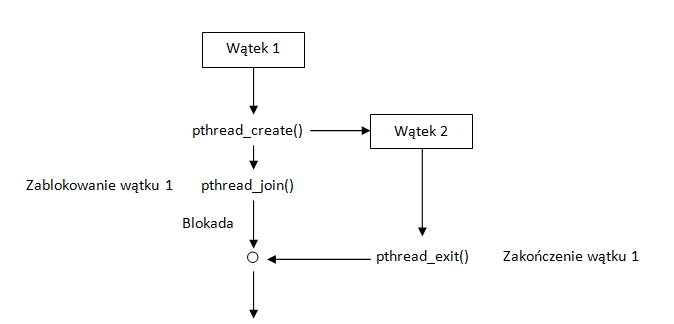
\includegraphics[width=0.85\textwidth]{img/laczenie1}
\caption{Łączenie wątków. Wątek 1 czeka na wątek 2}
\label{fig:laczenie1}
\end{figure}
\begin{figure}[!h]
\centering
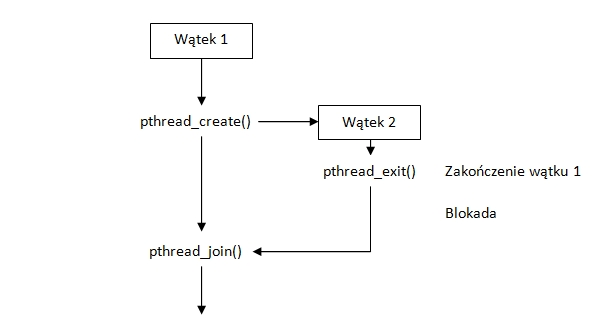
\includegraphics[width=0.85\textwidth]{img/laczenie2}
\caption{Łączenie wątków. Wątek 2 czeka na wątek 1}
\label{fig:laczenie2}
\end{figure}

\begin{example}{[Łączenie wątków]}
Przykład ilustruje omawiane zagadnienia łączenia wątków, wraz z~przekazaniem kodu powrotu z~utworzonych wątków do wątku głównego. 

\lstinputlisting[caption=Łączenie wątków,style=MyCStyle,label=src:thirdThread]{src/lab5/thirdThread.c}

\end{example} 


\subsubsection{Atrybuty wątków}

Biblioteka \lstinline[style=MyCStyle]{pthread} dostarcza mechanizmu do regulowania własności wątków. Atrybuty wątków są przekazywane jako parametry w~strukturze \lstinline[style=MyCStyle]{pthread_attr_t* attr} funkcji \lstinline[style=MyCStyle]{pthread_create()}, w~chwili tworzenia wątku. W~przypadku, gdy przekazujemy wskaźnik \lstinline[style=MyCStyle]{NULL}, atrybuty są ustawiane domyślnie. Jeśli chcemy utworzyć wątek, z~atrybutami innymi, niż domyślne, jawnie dobranymi przez użytkownika należy:


\begin{myitemize}
\item Utworzyć obiekt \lstinline[style=MyCStyle]{attr} typu \lstinline[style=MyCStyle]{pthread_attr_t}. 
\item Zainicjować zmienną \lstinline[style=MyCStyle]{attr} wywołaniem funkcji \lstinline[style=MyCStyle]{pthread_attr_init(&attr)}.
\item Zmodyfikować obiekt z~atrybutami, tak, aby zawierał pożądane wartości.
\item Przekazać wskaźnik do struktury \lstinline[style=MyCStyle]{attr}, w~trakcie tworzenia wątku za pomocą \lstinline[style=MyCStyle]{pthread_create()}. 
\item Zwolnić zasoby wykorzystywane przez atrybut, przez wywołanie funkcji \mbox{\lstinline[style=MyCStyle]{pthread_attr_destroy(&attr)}}.
\end{myitemize}

Wybrane atrybuty wątku przedstawiono w tabeli~\ref{tab:atrybuty1}, a~funkcje służące do ich ustawiania w~tabeli~\ref{tab:atrybuty2}.

\begin{table}[h!]
\centering
\caption{Wybrane atrybuty wątku i ich wartości domyślne}
\setlength{\arrayrulewidth}{1pt}
\setlength{\tabcolsep}{6pt}
\renewcommand{\arraystretch}{1.2}
\begin{tabular}{ |p{0.45\textwidth}|p{0.4\textwidth}| }
\hline \rowcolor{gray}
\textbf{Atrybut} & \textbf{Wartość domyślna} \\ \hline 
Dołączalność (\mbox{\lstinline[style=MyCStyle]{detachstate}}) & \mbox{\lstinline[style=MyCStyle]{PTHREAD_CREATE_JOINABLE}} \\ \hline
Dziedziczenie atrybutów (\mbox{\lstinline[style=MyCStyle]{inherit-scheduling}}) & \mbox{\lstinline[style=MyCStyle]{PTHREAD_INHERIT_SCHED}} \\ \hline 
Strategia szeregowania (\mbox{\lstinline[style=MyCStyle]{schedpolicy}}) & \mbox{\lstinline[style=MyCStyle]{PTHREAD_INHERIT_SCHED}} \\ \hline 
Parametry szeregowania (\mbox{\lstinline[style=MyCStyle]{schedparam}}) & Dziedziczone z procesu macierzystego \\ \hline 
Rywalizacja wątku o zasoby (\mbox{\lstinline[style=MyCStyle]{contentionscope}}) & \mbox{\lstinline[style=MyCStyle]{PTHREAD_SCOPE_SYSTEM}} \\ \hline 
Rozmiar stosu (\mbox{\lstinline[style=MyCStyle]{stacksize}}) & 4kB \\ \hline 
Adres stosu (\mbox{\lstinline[style=MyCStyle]{stackaddr}}) & \mbox{\lstinline[style=MyCStyle]{NULL}} \\ \hline 
\end{tabular}
\label{tab:atrybuty1}
\end{table}


Objaśnienia:

\begin{myitemize}
\item Dołączalność - informacja, czy wątek ma zwolnić zasoby natychmiast (\lstinline[style=MyCStyle]{PTHREAD_CREATE_DETACHED}), czy po wywołaniu przez proces macierzysty funkcji \lstinline[style=MyCStyle]{pthread_join (PTHREAD_CREATE_JOINABLE)}.
\item Dziedziczenie atrybutów - domyślnie są dziedziczone z~wątku macierzystego. 
\item Strategia szeregowania: \lstinline[style=MyCStyle]{SCHED_FIFO}, \lstinline[style=MyCStyle]{SCHED_RR}, \lstinline[style=MyCStyle]{SCHED_SPORADIC}, \lstinline[style=MyCStyle]{SCHED_OTHER} - szczegółowe objaśnienia w~dokumentacji.
\item Parametry szeregowania - informacje, dot. szeregowania wątków. Modyfikowana jest struktura \lstinline[style=MyCStyle]{const struct sched_param * param}. 
\item Rywalizacja wątku o~zasoby - wątki mogą rywalizować o~zasoby z~wątkami systemowymi z~innych procesów (ang. system contention scope).  Wątki mogą również rywalizować o~zasoby tylko w~obrębie procesu, który je utworzył (process contention scope). Domyślnie ustawiana jest pierwsza opcja. 
\item Rozmiar stosu - informacja o~rozmiarze stosu do przechowywania zmiennych lokalnych. 
\item Adres stosu - gdy adres stosu jest ustawiony na \lstinline[style=MyCStyle]{NULL}, to będzie ustalany i~zwalniany automatycznie przez system operacyjny. Pamięć na stos może być też przydzielona przez programistę i~wtedy jest on odpowiedzialny za jej zwolnienie. 
\end{myitemize}

Po inicjalizacji struktury z atrybutami, możemy pobierać i ustawiać atrybuty związane z wątkami. 

\begin{table}[h!]
\centering
\caption{Funkcje od pobierania i ustawiania atrybutów}
\setlength{\arrayrulewidth}{1pt}
\setlength{\tabcolsep}{6pt}
\renewcommand{\arraystretch}{1.2}
\begin{tabular}{ |p{0.25\textwidth}|p{0.35\textwidth}|p{0.35\textwidth}| }
\hline \rowcolor{gray}
\textbf{Atrybut} & \textbf{Pobierz atrybut} & \textbf{Ustaw atrybut} \\ \hline
Dołączalność & \mbox{\lstinline[style=MyCStyle]{pthread_attr_getdetachstate()}} & \mbox{\lstinline[style=MyCStyle]{pthread_attr_setdetachstate()}} \\ \hline 
Dziedziczenie atrybutów & \mbox{\lstinline[style=MyCStyle]{pthread_attr_getinheritsched()}} & \mbox{\lstinline[style=MyCStyle]{pthread_attr_setinheritsched()}} \\ \hline 
Strategia szeregowania & \mbox{\lstinline[style=MyCStyle]{pthread_attr_getschedpolicy()}} & \mbox{\lstinline[style=MyCStyle]{pthread_attr_setschedpolicy()}} \\ \hline 
Parametry szeregowania & \mbox{\lstinline[style=MyCStyle]{pthread_attr_getschedparam()}} & \mbox{\lstinline[style=MyCStyle]{pthread_attr_setschedparam()}} \\ \hline 
Rywalizacja o~zasoby & \mbox{\lstinline[style=MyCStyle]{pthread_attr_getscope()}} & \mbox{\lstinline[style=MyCStyle]{pthread_attr_setscope()}} \\ \hline 
Rozmiar stosu & \mbox{\lstinline[style=MyCStyle]{pthread_attr_getstacksize()}} & \mbox{\lstinline[style=MyCStyle]{pthread_attr_setstacksize()}} \\ \hline 
Adres stosu & \mbox{\lstinline[style=MyCStyle]{pthread_attr_getstackaddr()}} & \mbox{\lstinline[style=MyCStyle]{pthread_attr_setstackaddr()}} \\ \hline 
\end{tabular}
\label{tab:atrybuty2}
\end{table}


\begin{example}{[Atrybuty wątków]}
Przykład ilustruje omawiane zagadnienia łączenia wątków, wraz z~przekazaniem kodu powrotu z~utworzonych wątków do wątku głównego. 

\lstinputlisting[caption=Ustawianie atrybutu dołączalności,style=MyCStyle,label=src:attThread]{src/lab5/attThread.c}
\end{example} 

\subsubsection{Ustalanie priorytetu, strategii i parametrów szeregowania wątków}


\underline{Dziedziczenie atrybutów}


\noindent\textbf{Ustawianie atrybutów}. Wątki potomne domyślnie dziedziczą priorytet i~własności dotyczące szeregowania z~wątku macierzystego. Funkcja \lstinline[style=MyCStyle]{pthread_attr_setinheritsched} umożliwia zmianę tego stanu: 

\begin{lstlisting}[style=MyCStyle]
int pthread_attr_setinheritsched(pthread_attr_t * attr, int inheritsched );
\end{lstlisting}

gdzie \lstinline[style=MyCStyle]{attr} jest wskaźnikiem na strukturę definiującą atrybuty wątku, a~wartość \lstinline[style=MyCStyle]{inheritsched} jest jedną z~dwóch wartości: 

\begin{myitemize}
\item \lstinline[style=MyCStyle]{PTHREAD_INHERIT_SCHED} - wątek potomny dziedziczy strategię szeregowania od wątku rodzica - wartość domyślna.
\item \lstinline[style=MyCStyle]{PTHREAD_EXPLICIT_SCHED} - strategia szeregowania jest ustawiona przez strukturę \lstinline[style=MyCStyle]{attr}. 
\end{myitemize}

\noindent\textbf{Pobieranie atrybutów}. Funkcją, która umożliwia pobieranie parametrów dot. dziedziczenia własności z~wątku macierzystego ma następującą sygnaturę:  

\begin{lstlisting}[style=MyCStyle]
int pthread_attr_getinheritsched(const pthread_attr_t* attr,int* inheritsched );
\end{lstlisting}

gdzie wartość \lstinline[style=MyCStyle]{inheritsched} jest wskaźnikiem do miejsca, gdzie funkcja przechowa atrybut. 

\noindent\underline{Strategia szeregowania}
 
\noindent\textbf{Ustawianie atrybutów}. Ustawianie strategii szeregowania realizujemy funkcją: 

\begin{lstlisting}[style=MyCStyle]
int pthread_attr_setschedpolicy(pthread_attr_t* attr, int policy);
\end{lstlisting}

gdzie \lstinline[style=MyCStyle]{attr} jest wskaźnikiem na strukturę definiującą atrybuty wątku, a~wartość \lstinline[style=MyCStyle]{policy} jest jedną z~wartości zdefiniowanych w~tabeli~\ref{tab:sched}.

\begin{table}[h!]
\centering
\caption{Strategie szeregowania w QNX Neutrino}
\setlength{\arrayrulewidth}{1pt}
\setlength{\tabcolsep}{6pt}
\renewcommand{\arraystretch}{1.2}
\begin{tabular}{ |p{0.15\textwidth}|p{0.2\textwidth}|p{0.4\textwidth}| }
\hline \rowcolor{gray}
\textbf{Numer} & \textbf{Symbol} & \textbf{Opis} \\ \hline
\mbox{\lstinline[style=MyCStyle]{0}} & \mbox{\lstinline[style=MyCStyle]{SCHED_NOCHANGE}} & Brak zmiany strategii szeregowania \\ \hline 
\mbox{\lstinline[style=MyCStyle]{1}} & \mbox{\lstinline[style=MyCStyle]{SCHED_FIFO}} & Szeregowanie FIFO \\ \hline 
\mbox{\lstinline[style=MyCStyle]{2}} & \mbox{\lstinline[style=MyCStyle]{SCHED_RR}} & Szeregowanie karuzelowe \\ \hline 
\mbox{\lstinline[style=MyCStyle]{3}} & \mbox{\lstinline[style=MyCStyle]{SCHED_OTHER}} & wskazuje wartość \mbox{\lstinline[style=MyCStyle]{SCHED_RR}} \\ \hline 
\mbox{\lstinline[style=MyCStyle]{4}} & \mbox{\lstinline[style=MyCStyle]{SCHED_SPORADIC}} & Szeregowanie sporadyczne \\ \hline 
\end{tabular}
\label{tab:sched}
\end{table}

\noindent\textbf{Pobieranie atrybutów}. Pobieranie strategii szeregowania można zrealizować funkcją:

\begin{lstlisting}[style=MyCStyle]
int pthread_attr_getschedpolicy(const pthread_attr_t* attr,int* policy );
\end{lstlisting}

gdzie \lstinline[style=MyCStyle]{policy} jest wskaźnikiem do miejsca przechowywania ustawionej wartości strategii szeregowania. 

\noindent\underline{Parametry szeregowania}

\noindent\textbf{Ustawianie atrybutów}. Aby ustawić atrybuty z~tego zbioru należy zastosować funkcję: 

\begin{lstlisting}[style=MyCStyle]
int pthread_attr_setschedparam(pthread_attr_t * attr,const struct sched_param * param );
\end{lstlisting}

gdzie \lstinline[style=MyCStyle]{attr} jest wskaźnikiem na strukturę definiującą atrybuty wątku, a~zmienna \lstinline[style=MyCStyle]{param} jest wskaźnikiem na strukturę \lstinline[style=MyCStyle]{sched_param}, która definiuje parametry szeregowania watków. 

\noindent\textbf{Pobieranie atrybutów}. Tę funkcję realizujemy następująco: 

\begin{lstlisting}[style=MyCStyle]
int pthread_attr_getschedparam(const pthread_attr_t * attr, struct sched_param * param );
\end{lstlisting}

gdzie \lstinline[style=MyCStyle]{param} jest wskaźnikiem na strukturę \lstinline[style=MyCStyle]{sched_param}.

\begin{example}{[Zarządzanie atrybutami szeregowania wątków]}
Przykład pokazuje w~jaki sposób używać atrybutów, w~celu utworzenia wątku ze zdefiniowanymi przez programistę parametrami i~strategią szeregowania. 

\lstinputlisting[caption=Pobieranie i ustawianie atrybutów szeregowania wątków,style=MyCStyle,label=src:attThread]{src/lab5/sched.c}

Przykładowy wynik działania programu powinien wyglądać następująco: 

\begin{lstlisting}[style=MyCStyle]
Priorytet ustawiony przy starcie procesu (watku glownego) 10.
Domyslna strategia ROUND ROBIN, priorytet: 10
Domyslna strategia FIFO, priorytet: 8
Tworze watek z nowymi atrybutami: 
	Step = 0
	Step = 1
	Step = 2
	Step = 3
	Step = 4
Watek glowny dolaczyl watek potomny.
Watek glowny zakonczony. Wyjscie.
\end{lstlisting}

\end{example}


\subsection{Ćwiczenia}

\begin{myenumerate}
\item Napisać program, który tworzy $8$ wątków i~przekazuje do niego strukturę następującego typu:  

\begin{lstlisting}[style=MyCStyle]
struct thread_data 
{
	int	thread_id; /* ID watku */
	int sum; /* suma kontrolna */ 
	char *message;	 /* wiadomosc */
}
\end{lstlisting}

gdzie 

\begin{myitemize}
\item \lstinline[style=MyCStyle]{thread_id} - identyfikator wątku.
\item \lstinline[style=MyCStyle]{sum} - suma kontrolna, będąca sumą identyfikatorów wątków (np. dla pierwszego wątku \mbox{\lstinline[style=MyCStyle]{sum=0}}, dla drugiego \lstinline[style=MyCStyle]{sum=0+1}, dla trzeciego \lstinline[style=MyCStyle]{sum=0+1+2}, itd.). 
\item \lstinline[style=MyCStyle]{message} - wskaźnik, przechowujący wiadomość, otrzymaną z~programu głównego.   
\end{myitemize}

W programie głównym utworzyć tablicę o~następującej zawartości: 

\begin{lstlisting}[style=MyCStyle]
messages[0] = "English: Hello World!";
messages[1] = "French: Bonjour, le monde!";
messages[2] = "Spanish: Hola al mundo";
messages[3] = "Polski: Witaj swiecie!";
messages[4] = "German: Guten Tag, Welt!"; 
messages[5] = "Russian: Zdravstvytye, mir!";
messages[6] = "Japan: Sekai e konnichiwa!";
messages[7] = "Latin: Orbis, te saluto!";
\end{lstlisting}

Odpowiednie pola tablicy będą przekazywane do wątków. Każdy z~wątków powinien wyświetlać otrzymaną strukturę danych. Należy zadbać o~poprawne zakończenie wątków. 

\item Zaproponować współbieżną (równoległą - gdy dysponujemy komputerem wieloprocesorowym) wersję programu do obliczania liczby $\pi$ za pomocą wątków. Matematycznie wiadomo, że:

\begin{equation}\nonumber 
\displaystyle\int_0^1{\frac{4}{1+x^2}dx}=\pi
\end{equation}

Całkę oznaczoną możemy aproksymować jako sumę:

\begin{equation}\nonumber 
\sum_{i=0}^N\frac{4}{1+x_i^2}\Delta x\approx\pi
\end{equation}

Ilustrację graficzną aproksymacji liczby $\pi$ można znaleźć na rysunku~\ref{fig:piApprox}. 

\begin{figure}[!h]
\centering
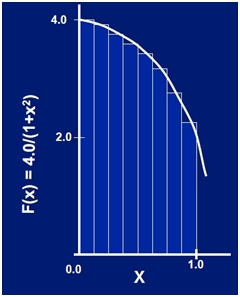
\includegraphics[width=0.4\textwidth]{img/piApprox}
\caption{Idea aproksymacji liczby $\pi$}
\label{fig:piApprox}
\end{figure}

\lstinputlisting[caption=Kod źródłowy sekwencyjnej wersji do obliczania liczby $\pi$,style=MyCStyle,label=src:piApprox]{src/lab5/piApprox.c}

\item Rozszerzyć poprzedni przykład o możliwość zmiany priorytetów i strategii szeregowania wątków.
\end{myenumerate} 


\cleardoublepage

\section{Mechanizmy synchronizacji wątków – muteksy, zmienne warunkowe, bariery}

\subsection{Wprowadzenie}
Zastosowanie obliczeń współbieżnych na ogół pozwala na osiągnięcie większej wydajności przetwarzania, w szczególności, gdy obliczenia są przeprowadzane na komputerach wieloprocesorowych. Pisanie poprawnie działających programów wielowątkowych wymaga specyfikacji i rozwiązania problemów, które w typowych obliczeniach sekwencyjnych nie występują. Problemy w~programowaniu współbieżnym biorą się z potrzeby synchronizowania wykonania wątków i zapewnienia im metod komunikowania się między sobą. Przy współbieżnym programowaniu należy zwrócić uwagę między innymi na następujące zagadnienia:

\begin{myitemize}
\item Wyścigi -- do sytuacji wyścigu (ang. race condition) dochodzi wówczas, gdy dwa lub więcej procesów (wątków) wykonuje operacje na zasobach współdzielonych, a ostateczny wynik tej operacji w sposób przypadkowy zależy od czasu realizacji ciągów instrukcji.
\item Spójność danych (ang. data consistency) -- współpracujące wątki mogą jednocześnie odczytywać i zapisywać te same obszary pamięci. Dostęp do wspólnego zasobu musi być synchronizowany, w celu zapewnienia spójności danych, w przeciwnym przypadku, rezultat przetwarzania może być inny, niż oczekiwany.
\end{myitemize}

Rozwiązaniem wymienionych problemów jest zastosowanie synchronizacji, czyli kontroli przepływu sterowania pomiędzy wątkami (procesami), tak, żeby dopuszczalne były tylko ciągi instrukcji, które są zgodne z intencjami. System operacyjny czasu rzeczywistego QNX Neutrino dostarcza wielu metod synchronizacji pracy wątków. Jedne dostarczają jawnych metod synchronizacji, takich jak muteksy (mutex), zmienne warunkowe (conditional variables), bariery (barriers), zamki wstrzymujące (sleepon lock), zamki czytelników i pisarzy (reader writer lock), semafory (semaphores). Drugą grupę stanowią metody niejawne, które gwarantują synchronizację, poprzez wbudowane mechanizmy. Należą do nich szeregowanie FIFO (FIFO scheduling), wysyłanie komunikatów (messages), operacje atomowe (atomic operations). Oprócz barier i blokad wstrzymujących wszystkie przytoczone mechanizmy pozwalają synchronizować nie tylko wątki, ale również procesy. Dodatkowym aspektem, który może mieć znaczenie jest możliwość synchronizacji wątków (procesów) w sieci. Spośród wymienionych metod semafory (nazwane) oraz komunikaty spełniają to wymaganie.
W trakcie laboratorium omówimy podstawowe operacje synchronizacji wątków (muteksy, zmienne warunkowe, bariery) oraz pojęcia z nimi związane (wzajemne wykluczanie, sekcja krytyczna, zakleszczenia, inwersja priorytetów). Rozważania będą ilustrowane przykładami pracy programów współbieżnych z zastosowaniem mechanizmów synchronizacji pracy wątków.

\subsection{Wyścigi}

Scenariusz, w którym występuje wyścig o współdzielony zasób przedstawia przykład. Wątek główny (wątek 1) wykonuje się współbieżnie z wątkiem 2. Oba wątki współdzielą zmienną \lstinline[style=MyCStyle]{b}. Problem pojawia się w sytuacji, gdy dwa wątki próbują ''jednocześnie'' zmodyfikować dane. W rezultacie wynik operacji będzie nieprzewidywalny i zależny od kolejności wykonania ciągów instrukcji przez poszczególne wątki. Jeden ze scenariuszy przedstawiono na rysunku~\ref{fig:race}.


\begin{figure}[!h]
\centering
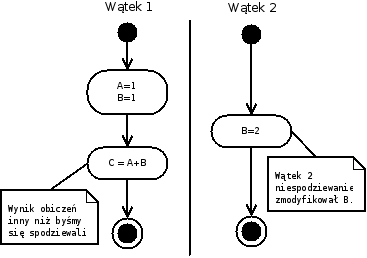
\includegraphics[width=0.5\textwidth]{img/thrd_race}
\caption{Ilustracja wyścigu (race condition) pomiędzy dwoma wątkami}
\label{fig:race}
\end{figure}

\begin{example}{[Brak synchronizacji pracy wątków]} \label{ex:nosynchro}
Skompilować, uruchomić kilkakrotnie program oraz zaobserwować różne scenariusze wykonania programu w~zależności od czasu pracy poszczególnych wątków.

\lstinputlisting[caption=Ilustracja braku synchronizacji pracy wątków,style=MyCStyle,label=src:racecond]{src/lab6/racecond.c}
\end{example}

\subsection{Muteksy}

Popularną i ogólną metodą synchronizowania pracy wątków jest zapewnienie dostępu do współdzielonych zasobów (np. pamięci) tylko dla jednego z potencjalnie wielu wykonywanych wątków lub procesów. Wymaganie to nazywa się wzajemnym wykluczaniem (ang. mutual exclusion). System QNX RTOS dostarcza zgodnego ze standardem POSIX mechanizmu wzajemnego wykluczania zwanego muteksem, który jest specjalną formą bardziej ogólnego mechanizmu semafora. Muteks jest rodzajem blokady, którą może zająć tylko jeden wątek jednocześnie. Jeśli jeden wątek zajął muteks i drugi w tym czasie próbuje zająć muteks, to będzie on w stanie zablokowanym (ang. locked). Muteks może być zwolniony tylko przez ten wątek, który go zajął. W tej sytuacji, wątek drugi jest w stanie odblokowanym (ang. unlocked). System operacyjny gwarantuje, że nie pojawią się wyścigi pomiędzy wątkami o zajęcie muteksu. Tylko jeden wątek może zająć muteks, pozostałe będą zablokowane. Ciąg instrukcji, który jest wykonywany tylko przez jeden, z potencjalnie wielu wątków (procesów) nazywamy \underline{sekcją krytyczną} (ang. critical section). Zasadę działania muteksu, w przypadku dwóch wątków, pracujących współbieżnie przedstawia rysunek~\ref{fig:mutex}.

\begin{figure}[!h]
\centering
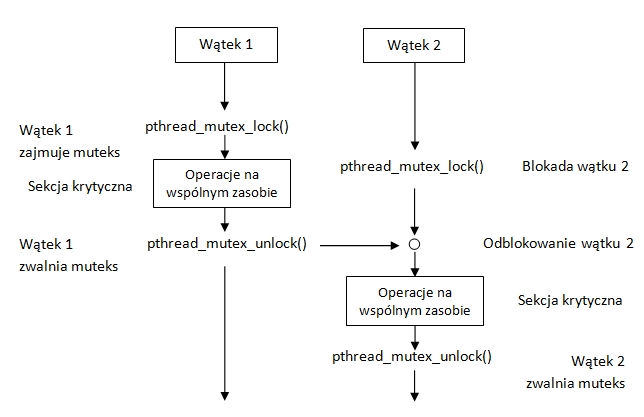
\includegraphics[width=0.85\textwidth]{img/mutex}
\caption{Zasada działania muteksów}
\label{fig:mutex}
\end{figure}

Typowy sposób użycia muteksu składa się z następujących operacji:

\begin{myenumerate}
\item Utworzenie muteksu (zmiennej typu \lstinline[style=MyCStyle]{pthread_mutex_t}) i~inicjalizacja.
\item Kilka wątków próbuje zająć muteks, tylko jednemu się udaje.
\item Wykonanie operacji na zasobie w sekcji krytycznej, przez wątek, który zajął muteks.
\item Zwolnienie muteksu.
\item Zajęcie muteksu i powtórzenie procesu.
\item Skasowanie muteksu.
\end{myenumerate}

\subsubsection{Tworzenie i kasowanie muteksów}

Muteks jest reprezentowany w programie za pomocą zmiennej \lstinline[style=MyCStyle]{pthread_mutex_t}. Funkcja \lstinline[style=MyCStyle]{pthread_mutex_init()} służy do inicjalizacji tego obiektu:

\begin{lstlisting}[style=MyCStyle]
pthread_mutex_t mutex = PTHREAD_MUTEX_INITIALIZER;

int pthread_mutex_init(
            pthread_mutex_t* mutex,
            const pthread_mutexattr_t* attr );
\end{lstlisting}


gdzie
\begin{myitemize}
\item \lstinline[style=MyCStyle]{mutex} -- jest wskaźnikiem do obiektu, który chcemy zainicjalizować.
\item \lstinline[style=MyCStyle]{attr} -- jest albo NULL (atrybuty domyślne) albo wskaźnikiem do struktury definiującej atrybuty muteksu.
\end{myitemize}

Muteksy możemy inicjalizować nie tylko dynamicznie, używając struktury \lstinline[style=MyCStyle]{attr}, ale również  statycznie, poprzez zastosowanie makra \lstinline[style=MyCStyle]{PTHREAD_MUTEX_INITIALIZER}, które zapewnia przypisanie domyślnych wartości do muteksu. Domyślnie muteks jest w stanie odblokowanym.
Do kasowania muteksu służy funkcja:

\begin{lstlisting}[style=MyCStyle]
int pthread_mutex_destroy( pthread_mutex_t* mutex );
\end{lstlisting}

Funkcja \lstinline[style=MyCStyle]{pthread_mutex_destroy()} kasuje zasoby zajęte przez muteks. Kasowany muteks powinien być w stanie odblokowanym. Zajęty muteks może być skasowany przez właściciela muteksu. W takim przypadku wątki czekające na muteksie zostają odblokowane.

\subsubsection{Zajmowanie i zwalnianie muteksów}

Funkcja  \lstinline[style=MyCStyle]{pthread_mutex_lock()} służy do zajęcia muteksu przez wątek. Jeśli muteks jest zajęty przez inny wątek, to pozostałe będą w stanie zablokowanym, aż do momentu, gdy muteks zostanie odblokowany. Gdy muteks jest wolny, to następuje jego zajęcie przez wątek bieżący.

\begin{lstlisting}[style=MyCStyle]
int pthread_mutex_lock( pthread_mutex_t* mutex );
\end{lstlisting}

gdzie mutex jest wskaźnikiem do obiektu typu \lstinline[style=MyCStyle]{pthread_mutex_t}. Zablokowane wątki mogą czekać dowolnie długo na odblokowanie muteksu. Funkcją, która umożliwia zajęcie muteksu na określony czas jest funkcja o~sygnaturze:

\begin{lstlisting}[style=MyCStyle]
int pthread_mutex_timedlock(
                  pthread_mutex_t * mutex,
                  const struct timespec * abs_timeout );
\end{lstlisting}

gdzie \lstinline[style=MyCStyle]{mutex} jest wskaźnikiem do obiektu typu \lstinline[style=MyCStyle]{pthread_mutex_t}, \lstinline[style=MyCStyle]{abs_timeout} wskaźnikiem do struktury:

\begin{lstlisting}[style=MyCStyle]
struct timespec {
   time_t   tv_sec;
   long     tv_nsec;
}
\end{lstlisting}

opisującej maksymalny czas, do którego ma czekać wątek, w celu odblokowania muteksu (czas absolutny).
Używanie funkcji \lstinline[style=MyCStyle]{pthread_mutex_lock()}, czy \lstinline[style=MyCStyle]{pthread_mutex_timedlock()} do zajęcia muteksu powoduje zablokowanie wątków wywołujących, gdy muteks jest zajęty. Na ogół taki stan jest pożądany. Zdarzają się jednak sytuacje, kiedy wątek zamiast czekać na zwolnienie muteksu, może wykonać użyteczne operacje. Biblioteka pthread dostarcza użytecznego mechanizmu \lstinline[style=MyCStyle]{pthread_mutex_trylock()}, który jest formą nieblokującego zajęcia muteksu.

\begin{lstlisting}[style=MyCStyle]
int pthread_mutex_trylock( pthread_mutex_t* mutex );
\end{lstlisting}

Funkcja \lstinline[style=MyCStyle]{pthread_mutex_trylock()} próbuje zająć muteks, ale nie blokuje wątków wywołujących, gdy muteks jest zajęty. Należy pamiętać, że aby odblokowywać muteks wówczas, kiedy funkcja \lstinline[style=MyCStyle]{pthread_mutex_trylock} zwróci kod sukcesu. Funkcja ta jest użyteczna, w przypadku zakleszczeń i sytuacji związanych z inwersją priorytetów. Funkcją, która pozwala na zwolnienie muteksu jest \lstinline[style=MyCStyle]{pthread_mutex_unlock()}:

\begin{lstlisting}[style=MyCStyle]
int pthread_mutex_unlock( pthread_mutex_t* mutex );
\end{lstlisting}

Funkcja \lstinline[style=MyCStyle]{pthread_mutex_unlock()} zwalnia muteks. Gdy istnieją wątki, które są zablokowane na muteksie, to zostaje odblokowany wątek, z najwyższym priorytetem i on staje się właścicielem muteksu. Gdy brak wątków zajmujących muteks, to stan muteksu zostaje ustawiony na wolny.

\begin{figure}[!h]
\centering
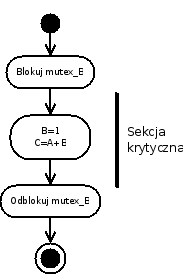
\includegraphics[width=0.3\textwidth]{img/thrd_mutex}
\caption{Przykład użycia muteksów}
\label{fig:mutex}
\end{figure}

\begin{example}{[Synchronizacja pracy wątków]}
Przykład jest modyfikacją przykładu~\ref{ex:nosynchro} i~pokazuje sposób użycia muteksu do ochrony wspólnych zasobów. Skompilować, uruchomić program oraz prześledzić jego działanie.

\lstinputlisting[caption=Przykład użycia muteksów,style=MyCStyle,label=src:mutex]{src/lab6/mutex.c}
\end{example}

\subsubsection{Problemy przy stosowaniu muteksów}

\textbf{Zakleszczenia}. Czasami użycie jednego muteksu do ochrony wspólnych danych jest niewystarczające. W przypadku jednoczesnego stosowania więcej niż jednego muteksu pojawiają się problemy, które nie występują, gdy stosujemy jeden muteks. Jednym z nich jest zakleszczenie (ang. deadlock), czyli sytuacja, gdy dwa (lub więcej wątków) czekają na siebie nawzajem, zajmując muteks (zasób) i jednocześnie czekają na zwolnienie innego muteksu (zasobu), zajętego przez inne wątki, potrzebnego do kontynuacji swojego działania. Klasyczną sytuacją jest scenariusz przedstawiony na rysunku~\ref{fig:deadlock}.

\begin{figure}[!h]
\centering
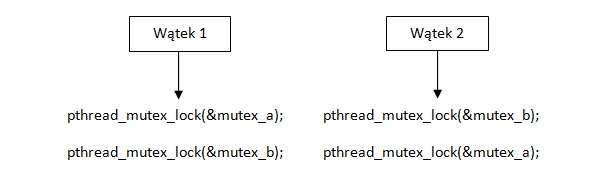
\includegraphics[width=0.8\textwidth]{img/deadlock}
\caption{Sytuacja zakleszczenia wątków (deadlock)}
\label{fig:deadlock}
\end{figure}

Oba wątki mogą ukończyć pierwszy etap scenariusza (zablokowanie na muteksach  \lstinline[style=MyCStyle]{mutex_a} oraz  \lstinline[style=MyCStyle]{mutex_b}) orientacyjnie w tym samym czasie. Jeśli ciąg instrukcji będzie taki, że np. wątek 2 najpierw zablokuje  \lstinline[style=MyCStyle]{mutex_b}, to wątek 1 zostanie zablokowany na muteksie, który jest już zajęty przez wątek 2, a następnie dojdzie do zablokowania wątku 2. Istnieją dwa typowe rozwiązania tego problemu:

\begin{myitemize}
\item Zajmowanie muteksów w ściśle określonej kolejności. (np. najpierw \lstinline[style=MyCStyle]{mutex_a}, a później \lstinline[style=MyCStyle]{muteks_b}).
\item Zastosowanie nieblokującej funkcji do zajmowania muteksu. Po zablokowaniu np. \lstinline[style=MyCStyle]{mutex_a}, używamy nieblokującej funkcji \lstinline[style=MyCStyle]{pthread_mutex_trylock()}, aby sprawdzić, czy \lstinline[style=MyCStyle]{mutex_b} jest zajęty; jeśli tak, to zwalniamy \lstinline[style=MyCStyle]{mutex_a} i~\lstinline[style=MyCStyle]{mutex_b} i powtarzamy całą procedurę.
\end{myitemize}

\begin{example}{[Zakleszczenie wątków]}
Przykład pokazuje zakleszczenie wątków. Skompilować i uruchomić program.

\lstinputlisting[caption=Deadlock,style=MyCStyle,label=src:asynchron]{src/lab6/deadlock1.c}
\end{example}

\begin{example}{[Użycie \texttt{pthread\_mutex\_trylock()} dla uniknięcia zakleszczenia wątków]}
Przykład pokazuje użycie funkcji \texttt{pthread\_mutex\_trylock()}. Skompilować i uruchomić program.

\lstinputlisting[caption=Nieblokujące próbkowanie muteksów (\texttt{thread\_mutex\_trylock()}),style=MyCStyle,label=src:asynchron]{src/lab6/deadlock2.c}
\end{example}

\textbf{Inwersja priorytetów}. Inwersja priorytetów jest problemem, który pojawia się w sytuacji, gdy występują conajmniej trzy wątki o różnych priorytetach. Istnieje wtedy konflikt pomiędzy wymaganiami nakładanymi przez metody synchronizacji (np. muteksy), a wymaganiami, dotyczącymi szeregowania wątków. Wykonywany jest wątek o niższym priorytecie, w sytuacji, gdy wątek o wyższym priorytecie został zablokowany na operacji synchronizacyjnej.

Przypuśćmy, że wątek 1, o najniższym priorytecie zajął muteks. Wątek 3, o najwyższym priorytecie, używa wspólnego zasobu z wątkiem 1 i próbuje zająć ten sam muteks poprzez wywołanie funkcji \lstinline[style=MyCStyle]{pthread_mutex_lock()}. Operacja nie udaje się i wątek 3 zostaje zablokowany na operacji synchronizacyjnej, mimo, iż ma wyższy priorytet, niż wątek 1. Jeśli pojawi się wątek 2 (np. na skutek aktywności innych wątków), o pośrednim priorytecie i wywłaszczy wątek 1, to wątek 1 nie będzie mógł zwolnić muteksu. Wówczas, wątek 3 będzie zablokowany na operacji synchronizacyjnej, a wątek 2 będzie się wykonywał, mimo, iż ma mniejszy priorytet, niż wątek 3.

W systemie QNX Neutrino są stosowane dwie strategie zapobiegania inwersji priorytetów:
\begin{myenumerate}
\item Dziedziczenie priorytetów polega na tymczasowym zwiększeniu priorytetu wątku, który posiada zasób (muteks) do najwyższego priorytetu wątku, który ubiega się o zasób. Priorytet wątku posiadającego zasób zostanie przywrócony do pierwotnego, po jego zwolnieniu. Schemat ten zapewnia, że wątki o najwyższych priorytetach będą zablokowane na najkrótszy możliwy czas, jednocześnie rozwiązując problem inwersji priorytetów.
\item Zastosowanie protokołu wykorzystującego pułap priorytetów -- polega na przydzieleniu zasobowi (muteksowi) priorytetu statycznego, większego od najwyższego priorytetu wątków, które o dany zasób będą konkurowały. Gdy jakiś wątek będzie próbował zająć zasób, to zostanie mu przydzielony tymczasowo priorytet związany z zasobem. Po zwolnieniu zasobu priorytet wątku wraca do wartości pierwotnej.
\end{myenumerate}

\subsection{Zmienne warunkowe}

\subsubsection{Wstęp}

Zmienne warunkowe dostarczają alternatywnego sposobu synchronizacji wątków. Podczas gdy muteksy synchronizują dostęp poszczególnych wątków do danych, zmienne warunkowe umożliwiają wątkom uzyskiwać informację (sygnalizować) o aktualnym stanie współdzielonych zasobów. Bez mechanizmu sygnalizowania zmiennych warunkowych, jeden z wątków musiałby nieustannie badać w pętli (potencjalnie w sekcji krytycznej) spełnienie pewnego warunku. Taki zabieg prowadziłby do niekorzystnego zużycia czasu procesora. Zmienna warunkowa pozwala osiągnąć ten sam cel bez użycia nieskończonej pętli.
Zmienna warunkowa jest mechanizmem sygnalizowania informacji i powinna być skojarzona z muteksem, który z kolei chroni dostępu do wspólnego zasobu (danych). Trzy podstawowe operacje dokonywane na zmiennych są następujące:

\begin{myitemize}
\item Oczekiwanie na zmienną warunkową (wait) – zwalnia muteks i zawiesza wątek aż do momentu zasygnalizowania zmiennej warunkowej.
\item Sygnalizowanie zmiennej warunkowej (signal) – sygnalizuje zmienną warunkową i wznawia zawieszony wątek.
\item Sygnalizowanie zmiennej warunkową (broadcast) – sygnalizuje zmienną warunkową i wznawia wszystkie wątki zawieszone w kolejce zmiennej warunkowej.
\end{myitemize}

Typowy scenariusz synchronizacji zmiennymi warunkowymi jest następujący:
\begin{myitemize}
\item Zadeklarować i zainicjalizować zmienną warunkową.
\item Zadeklarować i zainicjalizować stowarzyszony ze zmienną warunkową muteks.
\item Zablokować muteks stowarzyszony ze zmienną warunkową.
\item Kilka wątków zostaje zawieszonych w kolejce na zmiennej warunkowej i oczekują aż jakiś inny wątek zasygnalizuje sytuację sprzyjającą dalszej pracy.
\item Sygnalizacja zmiennej warunkowej.
\item Jeden z zawieszonych wątków (pierwszy w kolejce) wznawia swoje działanie. Pozostałe wątki oczekują nadal nad zmienną warunkową, aż do kolejnego zasygnalizowania zmiennej.
\item Odblokować muteks stowarzyszony ze zmienną warunkową.
\item Skasowanie muteksu.
\item Skasowanie zmiennej warunkowej.
\end{myitemize}


\subsubsection{Tworzenie i kasowanie zmiennych warunkowych}

Zmienna warunkowa jest reprezentowana w programie, jako zmienna typu \lstinline[style=MyCStyle]{pthread_cond_t} i musi być zainicjalizowana przed użyciem. Podobnie jak w przypadku muteksów istnieją dwa sposoby inicjalizacji statycznie, bądź dynamicznie.
\lstinline[style=MyCStyle]{pthread_cond_t cond = PTHREAD_COND_INITIALIZER;}

\begin{lstlisting}[style=MyCStyle]
int pthread_cond_init( pthread_cond_t* cond,
                       pthread_condattr_t* attr );
\end{lstlisting}

gdzie

\begin{myitemize}
\item \lstinline[style=MyCStyle]{cond} -- jest wskaźnikiem do zmiennej warunkowej \lstinline[style=MyCStyle]{pthread_cond_t}.
\item \lstinline[style=MyCStyle]{attr} -- jest albo \lstinline[style=MyCStyle]{NULL} (atrybuty domyślne) albo wskaźnikiem do struktury definiującej atrybuty muteksu.
\end{myitemize}


Zmienne warunkowe możemy inicjalizować nie tylko dynamicznie, używając struktury \lstinline[style=MyCStyle]{attr}, ale również  statycznie, poprzez zastosowanie makra \lstinline[style=MyCStyle]{PTHREAD_COND_INITIALIZER}, które zapewnia przypisanie domyślnych wartości do zmiennej warunkowej. Do kasowania zmiennej warunkowej służy funkcja:


\begin{lstlisting}[style=MyCStyle]
int pthread_cond_destroy( pthread_cond_t* cond );
\end{lstlisting}

Funkcja \lstinline[style=MyCStyle]{pthread_cond_destroy} kasuje zasoby zajęte przez zmienną warunkową.

\subsubsection{Czekanie i sygnalizowanie zmiennej warunkowej}

Funkcja \lstinline[style=MyCStyle]{pthread_cond_wait()} pozwala na oczekiwanie na zmienną warunkową:

\begin{lstlisting}[style=MyCStyle]
int pthread_cond_wait( pthread_cond_t* cond,
                       pthread_mutex_t* mutex );
\end{lstlisting}

gdzie

\begin{myitemize}
\item \lstinline[style=MyCStyle]{cond} -- jest wskaźnikiem do zmiennej warunkowej \lstinline[style=MyCStyle]{pthread_cond_t}.
\item \lstinline[style=MyCStyle]{mutex} -- stowarzyszony muteks.
\end{myitemize}

Funkcja \lstinline[style=MyCStyle]{pthread_cond_wait()} zawiesza wątek na zmiennej warunkowej \lstinline[style=MyCStyle]{cond}, ustawia go w kolejce wątków oczekujących i jednocześnie odblokowuje stowarzyszony muteks. Funkcja ta powinna być wywołana, wówczas kiedy muteks jest zajęty i automatycznie ponownie zamknie muteks po wyjściu z funkcji.

Istnieje odmiana funkcji, która pozwala czekać na zmiennej warunkowej przez określony czas:

\begin{lstlisting}[style=MyCStyle]
int pthread_cond_timedwait(
            pthread_cond_t* cond,
            pthread_mutex_t* mutex,
            const struct timespec* abstime );
\end{lstlisting}

gdzie
\begin{myitemize}
\item \lstinline[style=MyCStyle]{abstime} -- jest wskaźnikiem do struktury \lstinline[style=MyCStyle]{timespec}, która definiuje maksymalny absolutny czas blokowania wątku.
\end{myitemize}

Wątek w przypadku funkcji \lstinline[style=MyCStyle]{pthread_cond_wait()} lub \lstinline[style=MyCStyle]{pthread_cond_timedwait()} jest zablokowany do czasu zasygnalizowania zmiennej warunkowej przez  inny z wątków przez funkcję:

\begin{lstlisting}[style=MyCStyle]
int pthread_cond_signal( pthread_cond_t* cond );
\end{lstlisting}

Funkcja odblokowuje wątek o najwyższym priorytecie, który czeka na zmiennej warunkowej \lstinline[style=MyCStyle]{cond}. Gdy wątków o najwyższym priorytecie jest więcej, odblokowany będzie ten, który czeka najdłużej. Odblokowanie wszystkich wątków, które czekają na zmiennej warunkowej można zrealizować poprzez wywołanie funkcji:

\begin{lstlisting}[style=MyCStyle]
int pthread_cond_broadcast( pthread_cond_t* cond );
\end{lstlisting}

Wątki są odblokowane w zależności od wysokości priorytetów. W przypadku, gdy istnieje kilka wątków, o takich samych priorytetach, to wątki będą odblokowywane wg strategii FIFO. Działanie zmiennej warunkowej przedstawiono na rysunku~\ref{fig:condvar}.

\begin{figure}[!h]
\centering
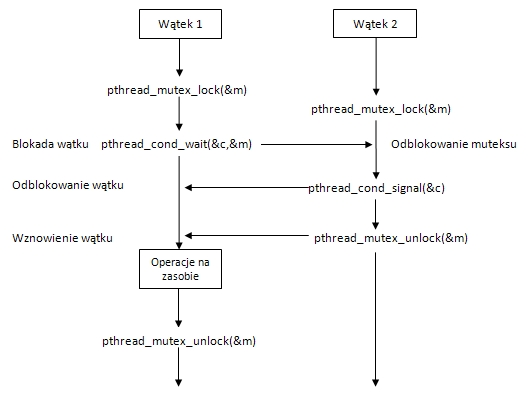
\includegraphics[width=0.75\textwidth]{img/condvar}
\caption{Idea działania zmiennej warunkowej}
\label{fig:condvar}
\end{figure}

\begin{example}{[Zmienne warunkowe]}
Program tworzy trzy wątki. Wątek główny pracuje jako zarządca (manager) i co 2 sekundy deleguje do pracy jeden z dwóch wątków wykonawczych. Realizacja zadania zajmuje każdemu z wątków wykonawców 3 sekundy. Skompilować program, uruchomić i prześledzić jego współbieżną pracę.
\lstinputlisting[caption=Zastosowanie zmiennej warunkowej,style=MyCStyle,label=src:condvar]{src/lab6/condvar.c}
\end{example}

\subsection{Bariery}

\subsubsection{Tworzenie i kasowanie bariery}

Synchronizacja przy użyciu bariery umożliwia koordynację pracy algorytmów. Bariera definiuje punkt w programie, do którego muszą dotrzeć wszystkie wątki zanim rozpoczną dalsze wykonanie. Liczba wątków potrzebnych do przełamania bariery jest definiowana w chwili tworzenia bariery.

\begin{figure}[!h]
\centering
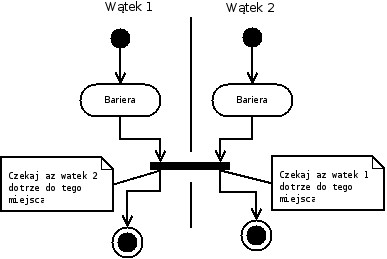
\includegraphics[width=0.5\textwidth]{img/thrd_barrier}
\caption{Idea działania bariery}
\label{fig:thrd_barrier}
\end{figure}

Bariera jest reprezentowana w programie, jako zmienna typu \lstinline[style=MyCStyle]{pthread_barrier_t} i musi być zainicjalizowana przed użyciem. Inicjalizacja bariery odbywa się poprzez wywołanie następującej funkcji:

\begin{lstlisting}[style=MyCStyle]
int pthread_barrier_init(
                    pthread_barrier_t * barrier,
                    const pthread_barrierattr_t * attr
                    unsigned int count );

\end{lstlisting}

gdzie

\begin{myitemize}
\item \lstinline[style=MyCStyle]{barrier} -- wskaźnik do obiektu typu \lstinline[style=MyCStyle]{pthread_barrier_t}, który chcemy zainicjalizować.
\item \lstinline[style=MyCStyle]{attr} -- jest albo \lstinline[style=MyCStyle]{NULL} (atrybuty domyślne) albo wskaźnikiem do struktury definiującej atrybuty bariery \lstinline[style=MyCStyle]{pthread_barrierattr_t}.
\item \lstinline[style=MyCStyle]{count} -- liczba wątków, które muszą dojść do momentu wywołania funkcji \lstinline[style=MyCStyle]{pthread_barrier_wait()}, aby wszystkie mogły kontynuować dalej swoje działanie.
\end{myitemize}

Bariery możemy inicjalizować nie tylko dynamicznie, używając struktury attr, ale również  statycznie, poprzez zastosowanie makra \lstinline[style=MyCStyle]{PTHREAD_BARRIER_INITIALIZER(count)}, które zapewnia przypisanie domyślnych wartości do bariery oraz liczby \lstinline[style=MyCStyle]{count}, omówionej poprzednio.

Do kasowania bariery służy funkcja:

\begin{lstlisting}[style=MyCStyle]
int pthread_barrier_destroy(
       pthread_barrier_t * barrier );
\end{lstlisting}

Funkcja \lstinline[style=MyCStyle]{pthread_barrier_destroy()} kasuje zasoby zajęte przez barierę.

\subsubsection{Czekanie na barierze}

Funkcja  \lstinline[style=MyCStyle]{pthread_barrier_wait()} pozwala na synchronizację wątków na barierze:

\begin{lstlisting}[style=MyCStyle]
	int pthread_barrier_wait( pthread_barrier_t * barrier );
\end{lstlisting}

Wątki, które wywołują funkcję są blokowane, aż do momentu, gdy wymagana liczba wątków (\lstinline[style=MyCStyle]{count}) wywołała funkcję \lstinline[style=MyCStyle]{pthread_barrier_wait()}, wówczas bariera jest przełamywana, jednemu z wątków (nieokreślonemu) jest zwracana wartość \lstinline[style=MyCStyle]{BARRIER_SERIAL_THREAD}, natomiast innym jest zwracana wartość zero. Po tym etapie stan bariery jest ustawiany do wartości po wywołaniu inicjalizacji bariery.

\begin{example}{[Brak synchronizacji]}
Program zawiera dwa wątki. Wątek 1 oblicza pewną wartość $a$, wątek 2 oblicza wartość $b$. Następnie wątek 1 powinien obliczyć $c=a+b$, a wątek 2 powinien obliczyć $d=a\cdot b$ -- zobacz rysunek~\ref{fig:thrd_async_example}. Przykład ilustruje brak synchronizacji pracy wątków.

\begin{figure}[!h]
\centering
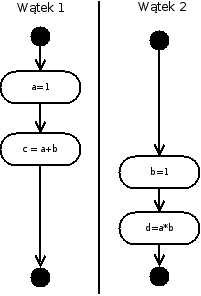
\includegraphics[width=0.35\textwidth]{img/thrd_async_example}
\caption{Idea działania bariery}
\label{fig:thrd_async_example}
\end{figure}

\lstinputlisting[caption=Brak synchronizacji pracy wątków,style=MyCStyle,label=src:nosynchro]{src/lab6/nosynchro.c}
\end{example}

\begin{example}{[Użycie bariery]} Poniższy przykład jest modyfikacją poprzedniego. Obliczenia zsynchronizowano używając bariery -- zobacz rysunek~\ref{fig:thrd_barrier_example}.

\begin{figure}[!h]
\centering
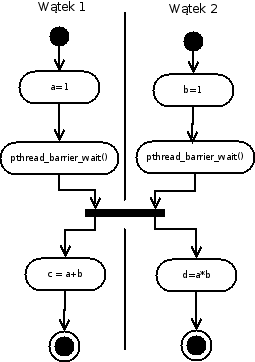
\includegraphics[width=0.35\textwidth]{img/thrd_barrier_example}
\caption{Idea działania bariery}
\label{fig:thrd_barrier_example}
\end{figure}

\lstinputlisting[caption=Brak synchronizacji pracy wątków,style=MyCStyle,label=src:synchrobarrier]{src/lab6/synchrobarrier.c}

\end{example}

\subsection{Ćwiczenia}

\begin{myenumerate}
\item Zaproponować współbieżną (równoległą – gdy dysponujemy komputerem wieloprocesorowym) wersję programu do obliczania liczby $\pi$ za pomocą wątków i mechanizmów synchronizacji. Matematycznie wiadomo, że:

\begin{equation}\nonumber
\displaystyle\int_0^1{\frac{4}{1+x^2}dx}=\pi
\end{equation}

Całkę oznaczoną możemy aproksymować jako sumę:

\begin{equation}\nonumber
\sum_{i=0}^N\frac{4}{1+x_i^2}\Delta x\approx\pi
\end{equation}

Ilustrację graficzną aproksymacji liczby $\pi$ można znaleźć na rysunku~\ref{fig:piApprox}. Należy zadeklarować sumę, jak zmienną globalną oraz obliczać ją w sekcji krytycznej. Synchronizację dostępu do zmiennej globalnej zapewnić poprzez zastosowanie muteksów.

\begin{figure}[!h]
\centering
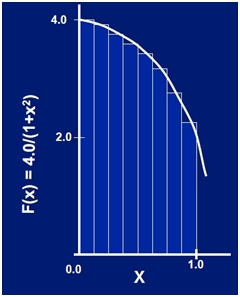
\includegraphics[width=0.4\textwidth]{img/piApprox}
\caption{Idea aproksymacji liczby $\pi$}
\label{fig:piApprox}
\end{figure}

\lstinputlisting[caption=Kod źródłowy sekwencyjnej wersji do obliczania liczby $\pi$,style=MyCStyle,label=src:piApprox]{src/lab6/piApprox.c}

\item Należy przeczytać tekst dot. inwersji prioryterów w~oprogramowaniu sondy marsjańskiej Pathfinder  \href{http://research.microsoft.com/en-us/um/people/mbj/mars\_pathfinder/Mars\_Pathfinder.html}{http://research.microsoft.com/en-us/um/people/mbj/mars\_pathfinder/Mars\_Pathfinder.html}.
\end{myenumerate}

\cleardoublepage

\section{Mechanizmy synchronizacji wątków – muteksy, zmienne warunkowe, bariery}

\cleardoublepage

\section{Mechanizmy komunikacji w systemie QNX Neutrino - komunikaty}



\cleardoublepage

\section{Mechanizmy komunikacji w systemie QNX Neutrino - komunikaty}



\cleardoublepage




\includepdf[scale=0.65,pages={1-4},pagecommand={\thispagestyle{fancy}{\section{Tworzenie oprogramowania dla urządzeń wbudowanych}}},nup=2x2,landscape=true]{img/bbb.pdf}

\includepdf[scale=0.85,pages={4-},pagecommand={\thispagestyle{fancy}{}},nup=2x2,landscape=true]{img/bbb.pdf}

 
\cleardoublepage


\clearpage

\tableofcontents

\renewcommand{\listtheoremname}{Spis przykładów}
\listoftheorems[ignoreall,show=example]


\cleardoublepage
\phantomsection
%% \addcontentsline{toc}{section}{Spis rysunków}
\listoffigures

\phantomsection
%% \addcontentsline{toc}{section}{Spis tabel}
\listoftables

\cleardoublepage
\bibliographystyle{plplain}
\nocite{*}
\phantomsection \label{pismiennictwo}
%% \addcontentsline{toc}{section}{Piśmiennictwo}
\bibliography{qnxlab}

\end{document}
